\documentclass[11pt]{article}
\usepackage[review]{acl}
\usepackage{times}
\usepackage{latexsym}
\usepackage[T1]{fontenc}
\usepackage[utf8]{inputenc}
\usepackage{microtype}
\usepackage{inconsolata}
\usepackage{graphicx}
\usepackage{booktabs}
\usepackage{placeins}
\usepackage{enumitem}
\setlist{itemsep=1.5pt,topsep=3pt,parsep=0pt,leftmargin=*}
\raggedbottom
\setlength{\emergencystretch}{1.5em}   % no overfull lines in long captions
\setlength{\textfloatsep}{9pt plus 2pt minus 2pt}
\setlength{\dbltextfloatsep}{10pt plus 2pt minus 2pt}
\brokenpenalty=10000
\hyphenation{Table Figure Appendix MMLU Original Deh-gha-ni}
\renewcommand{\dbltopfraction}{0.95}\renewcommand{\dblfloatpagefraction}{0.85}\setcounter{dbltopnumber}{3}
\renewcommand{\topfraction}{0.9}\renewcommand{\textfraction}{0.07}\renewcommand{\floatpagefraction}{0.85}
\usepackage{amsmath}
\usepackage{amssymb}
\usepackage{multirow}
\usepackage{xcolor}
\usepackage{colortbl}
\definecolor{oursbg}{gray}{0.91}
\definecolor{oursc}{HTML}{EB6834}
\newcommand{\cmark}{\checkmark}
\newcommand{\xmark}{$\times$}
\usepackage{url}
\def\UrlBreaks{\do\/\do-\do_\do.}
\usepackage{listings}
\lstset{language=Python,basicstyle=\fontsize{7.3pt}{8.5pt}\ttfamily\selectfont,columns=fixed,basewidth=0.45em,
  keepspaces=true,commentstyle=\color{gray},keywordstyle=\color{black},showstringspaces=false,frame=none,
  aboveskip=2pt,belowskip=2pt,xleftmargin=2pt}

\newcommand{\ci}[2]{\,{\scriptsize\ensuremath{[#1,\,#2]}}}
\newcommand{\nat}[1]{Original~#1/#1}
\newcommand{\up}[1]{$+#1$}
\newcommand{\dn}[1]{$-#1$}

\title{LoopBridge: Should Prefill and Decode Loop Equally?}

\author{Anonymous ACL submission}

\begin{document}
\raggedbottom
\maketitle

\begin{abstract}
Looped Transformers reuse a shared block across $n$ loops, yet inference stays costly because every generated token
repeats all $n$ passes sequentially. Cutting tied loops ($n/n$) hurts accuracy or collapses fixed-depth models.
Exploiting a sharp serving asymmetry---parallel prefill takes under 3\% of CoT wall time while sequential decode takes
over 97\%---we study \emph{asymmetric loop inference} ($m/n$, $m{>}n$). Naive untying exposes a \emph{contextual
representation shift} between deeper prompt caches and shallow decode passes, degrading retrieval on variable-depth
models and collapsing fixed-depth models or $n{=}1$. We introduce \emph{LoopBridge}, an asymmetric-loop adapter with
two zero-decode-overhead modules: a \emph{learnable prompt KV bridge} folded once at prefill, plus statically
\emph{merged decoder LoRA} when decode dynamics need adaptation. On 26.4B sparse-MoE Inkling-2 in Day-0 vLLM (29 arms,
124,816 rollouts to 1M) and 1.4B--2.6B Ouro: on variable-depth \texttt{TML-d24-varloop} ($n{\ge}2$), the
0.017--0.025\% KV bridge \emph{alone} ($r{=}0$) lifts 4/2 by $+2.8$ ($+9.5$ MRCR~512K) at $1.75\times$ decode speed
and recovers 99.0\% of 4/4 at 4/3 ($1.27\times$), while one 0.042\% zero-synthetic universal adapter hits 69.8\% at
3/2; on fixed-depth models and $n{=}1$, merged LoRA beats tied distillation by $+5.7$ on \texttt{Inkling-2-Mini}~3/2,
$+5.3$ on \texttt{TML-varloop}~3/1 ($p{<}10^{-4}$), and $+8.7$ on Ouro-2.6B~4/1 ($4.2\times$). On 1$\times$B300
multi-turn grids, BFCL~v4 (15,200 episodes), and SWE-bench Verified, naive re-prefill loses speed and accuracy on
short-output tasks, whereas prefix-cached policies sustain $1.50$--$1.78\times$ speedups and preserve 2/2 accuracy
without LoRA drift ($+6.3$ BFCL, $p{=}0.012$), while upgrading shallow turns (Policy~I semantics) beats Mini tied KD
by $+7.8$ (BFCL) and lifts 1-loop SWE-bench from 32\% (40\% distilled) to 70\% ($p{<}10^{-4}$).
\end{abstract}

\section{Introduction}
\label{sec:intro}

\begin{figure}[t]
\centering
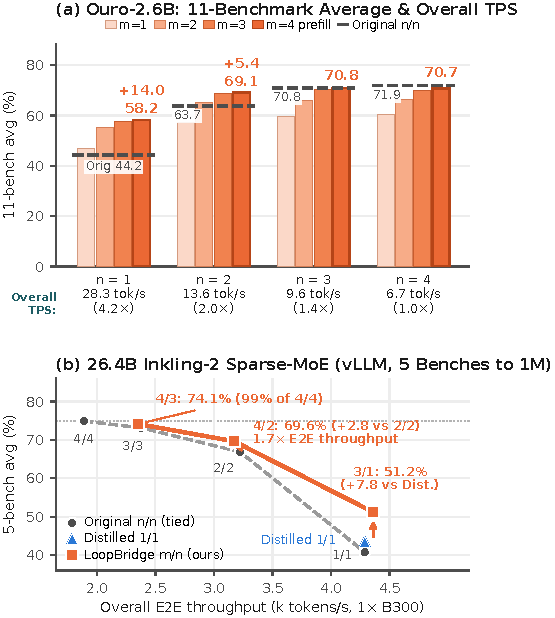
\includegraphics[width=0.98\columnwidth]{../figs/fig_tps_teaser.pdf}
\caption{\textbf{Asymmetric loop inference ($m/n$: $m$ prefill / $n$ decode loops, $m{>}n$) shifts the accuracy--throughput frontier across 2.6B dense
and 26.4B sparse-MoE backbones} (1$\times$B300). (a)~Ouro-2.6B 11-benchmark average over all 16 $(m,n)$ pairs with
overall end-to-end throughput (\mbox{tok/s}, batch~1, 4 CoT tasks; LB 4/1 = 27.7, 4/2 = 14.3): $m{=}4$ adds $+14.0$ at
$n{=}1$ ($4.2\times$) and $+5.4$ at $n{=}2$ ($2.0\times$), while $m{<}n$ hurts. (b)~26.4B \texttt{TML-d24-varloop} in
Day-0 vLLM (5 benchmarks to 1M, $5\times$avg@4, Orig~1/1 @1; E2E $L{=}512, B{=}16$): KV-only 4/3 recovers 99.0\% of
4/4, 4/2 beats 2/2 by $+2.8$ ($1.7\times$), and 3/1 beats Distilled~1/1 by $+5.3$ ($p{<}10^{-4}$).}
\label{fig:teaser}
\end{figure}

Looped Transformers~\citep{ut} reuse a shared block of layers across recurrent passes per token, scaling effective depth
and reasoning quality without adding parameters---from dense 1.4B--2.6B checkpoints such as Ouro~\citep{ouro} to frontier
26.4B sparse-MoE models such as Thinking Machines' Inkling-2 family (\texttt{TML-d24-varloop} and
\texttt{Inkling-2-Mini}, 1M context)~\citep{inkling2}. Yet looped models remain costly to serve because every generated
token repeats all $n$ passes sequentially.

Reducing the tied loop count ($n/n$) speeds up generation at a steep quality cost: halving loops from 4/4 to 2/2 drops
8.2 points on Ouro-2.6B and 8.0 points on \texttt{TML-d24-varloop}, while fixed-depth models such as
\texttt{Inkling-2-Mini} collapse outright (Figure~\ref{fig:teaser}, Section~\ref{sec:inkling_main}).

This trade-off ignores a sharp latency asymmetry between prefill and decode. Parallel prefill runs once per prompt and
takes under 3\% of batch-1 chain-of-thought runtime, whereas sequential decoding accounts for over 97\%
(Figure~\ref{fig:method}, top; Appendix~\ref{app:time}). This motivates \emph{asymmetric loop inference}: reading the
prompt with more loops ($m$) to build rich contextual representations while generating answer tokens with fewer loops
($n{<}m$). We write $m/n$ for $m$ prefill and $n$ decode loops, and \emph{Original~$n/n$} for the released model with
$n$ tied loops. Unlike deep-encoder/shallow-decoder architectures~\citep{deepshallow}, one frozen looped backbone plays
both roles.

Directly untying prefill and decode without adaptation, however, exposes a \emph{contextual representation shift}: each
decode loop $k$ now attends to prompt KV states produced at a deeper prefill pass than seen during pretraining.
Empirically, the shift manifests differently depending on whether the backbone extrapolates across loop depths:
(i)~on \emph{variable-depth} backbones (\texttt{TML-d24-varloop} at $n{\ge}2$), training-free untying yields partial
gains without crashing but leaves a cross-depth prompt KV mismatch on 256K--1M retrieval
(Figure~\ref{fig:inkling_main}a);
(ii)~on \emph{fixed-depth} backbones (Ouro-2.6B, \texttt{Inkling-2-Mini}) or un-gated $n{=}1$, naive untying severely
degrades or collapses (\texttt{Inkling-2-Mini}~3/2 drops to 2.2\% with 93\% truncation; Ouro-2.6B~4/1 falls from 44.2 to
28.7; Table~\ref{tab:main}).

To bridge this shift over a frozen backbone, we introduce \emph{LoopBridge}, an asymmetric-loop distillation method with
two zero-decode-overhead modules (Section~\ref{sec:method}, Figure~\ref{fig:method}):
\begin{enumerate}
\item \textbf{Learnable Prompt KV Bridge ($M^K, M^V$)} projects $m$-loop prompt KV states into each decode loop's
subspace (RoPE-commuting key scales and linear value maps on Ouro; global-3 residual maps on NoPE Inkling-2). Folded
\emph{once} at prefill, it adds 0\% decode compute; on variable-depth 26.4B MoEs at $n{\ge}2$, this 0.017--0.025\%
bridge \emph{alone} ($r{=}0$, frozen decoder) closes the shift without decode-weight drift.
\item \textbf{Merged Decoder LoRA} adapts decode dynamics when backbones cannot extrapolate to shallow decode depths
(fixed-depth models or $n{=}1$), statically merged before serving for 0\% decode overhead.
\end{enumerate}

In \emph{multi-turn and agentic} serving, turn $t{-}1$'s shallow-decoded answer $A_{t-1}$ re-enters turn $t$'s prompt.
Should the server re-prefill the full history, keep dual states for incremental re-prefill, or reuse folded prefixes
under Automatic Prefix Caching (APC)? We derive exact KV and sliding-window memory costs and evaluate all policies on
1$\times$B300 grids, BFCL~v4 Multi-Turn (15,200 episodes), and official SWE-bench Verified (Section~\ref{sec:multiturn}).

Across 26.4B Inkling-2 (29 five-benchmark arms, 124,816 rollouts), dense 1.4B--2.6B Ouro and Thinking models, and Lev
decision models, our contributions are:
\begin{itemize}
\item \textbf{26.4B Inkling-2 (Day-0 vLLM):} On \texttt{TML-d24-varloop} ($n{\ge}2$), the $r{=}0$ KV bridge lifts 4/2 by
$+2.8$ ($+9.5$ MRCR~512K, $+2.0$ LBv2~1M) at $1.75\times$ decode speed and recovers 99.0\% of 4/4 at 4/3 ($1.27\times$),
verified by a 4-cell $2{\times}2$ causal factorial and matched $r{=}64$ twins; one 0.042\% zero-synthetic universal
adapter serves 4/3, 4/2, and 3/2 (69.8\% at 3/2). On fixed-depth \texttt{Inkling-2-Mini}~3/2 and \texttt{TML-varloop}~3/1,
LoopBridge beats 24M tied distillation by $+5.7$ and $+5.3$ ($p{<}10^{-4}$).
\item \textbf{Dense Ouro \& Lev:} On Ouro-2.6B, LoopBridge lifts 4/1 to 58.2 ($+8.7$ over Distilled~1/1, $4.2\times$
speed) and 4/2 to 69.1 ($+5.4$ over 2/2, $2.0\times$); Thinking~4/2 matches 4/4 on GSM8K at $2.0\times$ throughput.
\item \textbf{Multi-Turn \& Agentic Serving:} Naive re-prefill drops to $0.52\times$ on short-output tasks, whereas
prefix-cached \emph{Policy~APC-D0} sustains $1.50$--$1.78\times$ speedups (zero dual-KV) and preserves 2/2 accuracy
without LoRA drift ($+6.3^\ast$ BFCL~v4, $p{=}0.012$), while upgrading $A_{t-1}$ (\emph{Policy~I} semantics) beats Mini
tied KD by $+7.8^\ast$ (BFCL) and lifts 1-loop SWE-bench from 32\% (40\% distilled) to 70\% ($p{<}10^{-4}$), alongside
honest fixed-depth coding boundaries.
\end{itemize}

\begin{figure*}[t]
\centering
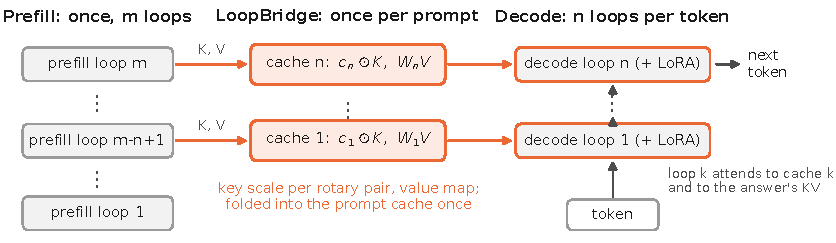
\includegraphics[width=0.77\textwidth]{../figs/fig0_method.pdf}
\caption{\textbf{Asymmetric loop inference and LoopBridge architecture} (RoPE Ouro and NoPE 26.4B Inkling-2).
\emph{Top:} batch-1 CoT prefill takes $<3\%$ of runtime vs.\ $>97\%$ decode, making deeper prefill ($m{>}n$) nearly
free. \emph{Bottom:} the frozen backbone prefills with $m$ loops; once per prompt, the \emph{KV Bridge} folds mapped
caches into $n$ decode caches ($c_k{\odot}K, W_k V$ on Ouro; global-3 $I{+}\Delta_{k,p}$ on Inkling-2), running $n$-loop
decode at native speed with 0\% KV-map compute (frozen decoder on variable-depth MoEs at $n{\ge}2$; merged LoRA on
fixed-depth/$n{=}1$; Figure~\ref{alg:loopbridge}).}
\label{fig:method}
\end{figure*}

\section{Related Work}
\label{sec:related}

\paragraph{Looped models.} Looped Transformers~\citep{ut,huginn,ouro,relaxedrecursive,mor} reuse a shared block for
effective depth and latent reasoning~\citep{saunshi2025latent}. Relaxed Recursive Transformers~\citep{relaxedrecursive}
add per-loop LoRA, while ELR, Dory, and Ouro's KV-sharing mode retain only the final loop's cache~\citep{elr,dory,ouro}
(Ouro loses $>10$ GSM8K points if reused in prefill). All tie prefill and decode loops; we untie them within one frozen
backbone.

\paragraph{Phase-asymmetric depth and KV alignment.} Continuous Depth Batching~\citep{cdb} and early
exit~\citep{calm,layerskip} vary depth per token. Concurrent LoopDuet~\citep{loopduet} tests training-free untying on
Huginn and OLMo-2 with $m{\le}n$ (our Huginn-0125 checks found no GSM8K gain); across four families, $m{>}n$ dominates
while $m{<}n$ hurts. Asymmetric phase capacity also appears in width pruning~\citep{overfill}, two-network
designs~\citep{deepshallow,llm2slm,tandem,bridgekv}, and shallower prefill~\citep{swiftkv}; speculative
decoding~\citep{specdecoding,specsampling} and disaggregation~\citep{distserve,splitwise} are complementary. Unlike
YOCO~\citep{yoco}, KITE~\citep{kite}, and Plato's Key~\citep{platoskey}, LoopBridge aligns caches across loop depths of
one frozen backbone (Appendix~\ref{app:related}).

\section{Method}
\label{sec:method}

\subsection{Asymmetric Loop Inference and Contextual Shift}

A looped language model applies a shared layer block across $m$ recurrent passes during prefill and $n$ passes per
generated token during decode, maintaining a KV cache per loop and layer. In standard serving ($m{=}n$, \emph{Original~$n/n$}),
increasing prefill from 1 to $m$ loops scales total latency only by $(m{-}1)p$ for prefill share $p$, whereas cutting
decode from $m$ to $n$ saves $(m{-}n)/m$ of decode compute on every generated token. Whenever $p$ is small
(Section~\ref{sec:time}), asymmetric inference ($m{>}n$) provides deep prompt encoding at shallow decode cost.

To untie the two phases, prefill runs $m$ loops up to the penultimate prompt token; the final prompt token and all
generated tokens run $n$ decode loops. Decode loop $k\in\{1,\dots,n\}$ reads prompt KV from paired prefill loop $j(k)$:
standard \emph{tail pairing} sets $j(k){=}\max(m{-}n{+}k,1)$ (aligning the final pass and recovering Original~$n/n$ when
$m{=}n$), while on hybrid sandwich-looped Inkling-2 MoEs---where loop~1 omits inter-loop message gates---we also evaluate
\emph{anchored pairing} ($j(1){=}1$, $j(k){=}m{-}n{+}k$ for $k{\ge}2$).

When $m{\neq}n$, decode loop $k$ attends to prompt KV representations generated at a different recurrence depth than it
saw during pretraining. This \emph{contextual representation shift} degrades retrieval on variable-depth models and
triggers severe degradation or output collapse on fixed-depth models and un-gated $n{=}1$ decoders
(Table~\ref{tab:main}, Figure~\ref{fig:inkling_main}).

\subsection{LoopBridge: KV Bridge and Merged Decoder LoRA}

LoopBridge resolves this mismatch over a \emph{100\% frozen backbone} via two zero-decode-overhead modules
(Figure~\ref{fig:method}; pseudocode in Appendix~\ref{app:method}):

\paragraph{Learnable Prompt KV Bridge ($M^K, M^V$).}
To align $m$-loop prompt representations with the subspace expected by decode loop $k$, we attach identity-initialized
linear maps acting solely on the prompt KV cache:
\begin{itemize}
\item \emph{RoPE backbones (Ouro):} For each decode loop $k$, layer, and KV head, a complex scalar $c_k$ per rotary
frequency pair scales and rotates keys while commuting with RoPE~\citep{rope} (preserving relative-position invariance),
paired with a $d_h{\times}d_h$ linear value map $W_k$.
\item \emph{Hybrid NoPE backbones (Inkling-2):} Because Inkling-2 concentrates long-range attention into four global
NoPE layers (L5 pre-loop; L11, L17 looped; L23 post-loop) with additive position bias~\citep{inkling2}, LoopBridge
applies unconstrained cross-pass residual maps $K'_j = K_j + \sum_{p=1}^m \Delta^K_{k,p} K_p$ (and analogously $V'_j$)
exclusively to the three looped/post-loop global layers (L11, L17, L23).
\end{itemize}
Crucially, both formulations are \emph{folded once} into the prompt KV cache at the end of prefill, incurring zero
compute per decode step. On variable-depth 26.4B MoEs at $n{\ge}2$, training \emph{only} this KV bridge (\emph{KV-Only},
$r{=}0$, 4.46--6.55M parameters = 0.017--0.025\% of 26.4B) with the decoder completely frozen resolves contextual shift
while avoiding any decode-weight drift. An optional \emph{one-cache} Ouro variant maps only the last prefill loop to cut
prompt KV memory $n\times$ (Table~\ref{tab:ablate}a).

\paragraph{Merged Decoder LoRA.}
When the backbone cannot extrapolate natively to shallower decode depths (fixed-depth models such as Ouro and
\texttt{Inkling-2-Mini}, or $n{=}1$), aligning prompt KV alone is insufficient because decode-step hidden dynamics
themselves were never trained for $n$ passes. We attach decode-only LoRA~\citep{lora} (rank 16 on Ouro; rank 64 on
Inkling-2) active strictly during decoding, and statically merge it into base projections prior to serving---preserving
exact native $n$-loop per-token latency.

\subsection{Asymmetric-Loop Distillation}

We distill LoopBridge via forward KL divergence $\mathrm{KL}(p_{\text{teacher}} \,\|\, p_{\text{student}})$ over answer
positions from the frozen full-depth backbone ($4/4$ on Ouro and \texttt{TML-d24-varloop}; $3/3$ on
\texttt{Inkling-2-Mini}). On Ouro-2.6B, one 63.3M-parameter adapter (2.4\%) trains on 48M answer tokens sampling random
$(m,n)\in\{1..4\}^2$ to serve all 16 pairs (Appendix~\ref{app:training}). On 26.4B Inkling-2, variable-depth
\emph{KV-Only} ($r{=}0$, 0.017--0.025\%) trains on 12M pure on-policy $4/4$ rollouts (plus a 0\%-synthetic natural-only
ablation and one 0.042\% multi-depth universal checkpoint serving 4/3, 4/2, and 3/2), while fixed-depth and $n{=}1$
controls use locked 24M-token $r{=}64$ budgets (34.6--39.9M vs.\ 43.7--47.4M for tied Distilled baselines;
Appendix~\ref{app:inkling}).

\subsection{Multi-Turn and Agentic Serving Policies}
\label{sec:mt_method}

In multi-turn chat and tool-use agents, turn $t{-}1$'s shallow-decoded response $A_{t-1}$ (computed with $n$ loops) and
new user/tool observation $U_t$ become part of the prompt $H_t = [H_{t-1}, A_{t-1}, U_t]$ on turn $t$. Standard tied
engines reuse $H_{t-1}$ and $A_{t-1}$ via Automatic Prefix Caching (APC) and prefill only $U_t$. Under asymmetric
inference ($m{>}n$), handling $[A_{t-1}, U_t]$ exposes a four-way systems--accuracy spectrum (exact state formulas on
24-layer Inkling-2, which has 20 local SWA/SConv layers and only 4 global full-attention layers at $4\text{ KiB/tok/slot}$):
\begin{enumerate}
\item \textbf{Policy~R (Full Re-Prefill, APC off):} Discards prior caches and re-prefills all of $H_t$ with $m$ loops
plus KV folding every turn ($2{+}2m$ global slots, $O(m T^2)$ recompute).
\item \textbf{Policy~I (Incremental Dual-State; analytical):} Retains raw $m$-pass global KV ($2{+}2m$ slots) plus
folded $n$-pass KV ($1{+}2n$ on L11/L17/L23), totaling $3{+}2m{+}2n$ global slots ($+37.5\%$/$+50\%$/$+62.5\%$ for
3/1, 4/2, 3/2) plus $O(1)$ SWA/SConv state ($(10{+}10m){\times}4\text{ MiB} = 160/200\text{ MiB}$). Incrementally
prefills and folds only $[A_{t-1}, U_t]$ ($O(m(|A_{t-1}|{+}|U_t|))$); unimplemented in vLLM (accuracy via exact
Policy~R, incremental prefill bounded in Table~\ref{tab:mt_systems}).
\item \textbf{Policy~APC-D0 (Turn-0 Fold + APC):} Standard vLLM APC with zero dual-KV ($2{+}2m$ slots, matching
Orig~$m/m$). Turn~0 folds once; turns $t{\ge}1$ reuse prefixes (91.3--96.6\% APC on agentic suites; 83.6--83.7\% on
grids), write unfolded $m$-pass KV on $[n_{\text{comp}}, |H_t|)$ (read via paired passes), and decode with $n$-pass CUDA
graphs.
\item \textbf{Policy~APC-S (Suffix-Only Fold):} Extends APC-D0 by folding newly allocated block-aligned suffix blocks
$[n_{\text{comp}}, |H_t|)$ ($<1\text{ ms}$, zero extra memory, cached prefix untouched), isolating folding $U_t$ vs.\
upgrading $A_{t-1}$.
\end{enumerate}

\section{Experimental Setup}
\label{sec:setup}

\paragraph{Models and benchmarks.} We evaluate four families spanning $10\times$ in scale:
(i)~\textbf{26.4B sparse-MoE Inkling-2}~\citep{inkling2} (\texttt{TML-d24-varloop} and fixed-3 \texttt{Inkling-2-Mini})
in Day-0 Blackwell vLLM~\citep{vllm} on five reasoning and 256K--1M benchmarks---GPQA Diamond~\citep{gpqa},
LiveCodeBench~v6~\citep{livecodebench}, MRCR~v2 8-needle 256K--512K~\citep{openai_mrcr}, GraphWalks
BFS~256K~\citep{openai_mrcr}, and LongBench~v2~1M~\citep{longbenchv2} (29 full $5\times$avg@4 arms = 124,816
rollouts)---plus \textbf{BFCL~v4 Multi-Turn} (\texttt{base} 200 + \texttt{long\_context} 200, avg@2 = 15,200 executable
episodes across 19 arms) and official \textbf{SWE-bench Verified} (\texttt{mini-swe-agent} bash-only, official
\texttt{swebench.harness.grading}, 19 arms across 50 gold-verified tasks; Appendix~\ref{app:multiturn});
(ii)~\textbf{dense 1.4B--2.6B Ouro} and Thinking~\citep{ouro} on 11 benchmarks (MMLU, MMLU-Pro, BBH, ARC-C, HellaSwag,
Winogrande, GSM8K, MATH-500, HumanEval+/MBPP+, RULER-16K; plus HELMET on Thinking; Appendix~\ref{app:eval});
and (iii)~\textbf{Lev} decision models~\citep{lev} (Section~\ref{sec:others}).

\paragraph{Controls and timing.} All controls keep the backbone frozen: \emph{Original~$n/n$}, \emph{Training-free~$m/n$},
tied \emph{Distilled~$n/n$} (matched corpus, teacher, and tokens), plus matched $r{=}0$ \emph{KV-Only~2/2} (with/without
synthetic data) and $r{=}64$ twins on Inkling-2. Timing uses isolated 1$\times$B300 runs; paired CIs use 95\%
item-clustered bootstrap (5,000 resamples).

\begin{figure*}[t]
\centering
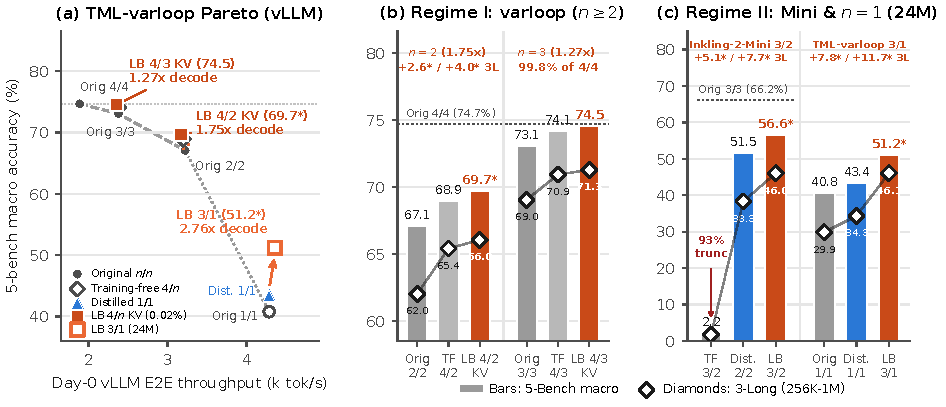
\includegraphics[width=0.90\textwidth]{../figs/fig_inkling_main.pdf}
\caption{\textbf{Contextual shift and causal controls on 26.4B sparse-MoE Inkling-2 in Day-0 vLLM} (5 official
benchmarks to 1M; solid: 5-Bench Avg; hatched: 3-Long Avg 256K--1M; $^\ast$95\% clustered CI excludes zero).
(a)~\emph{Variable-depth \texttt{TML-d24-varloop} ($n{\ge}2$, $5\times$avg@4):} at $n{=}2$ ($1.75\times$), Tied~KV~2/2
stays flat (67.0\%) and $10.5\times$-larger Distilled~2/2 (68.9\%$^\ast$) merely ties zero-shot 4/2 (68.9\%$^\ast$),
whereas 0.017\% KV-only ($r{=}0$) reaches 69.6\%$^\ast$ ($+2.7^\ast$ vs.\ Tied~KV, tying $r{=}64$ LB~4/2) and 0.042\%
0\%-synth Universal~3/2 leads at 69.8\%$^\ast$; at $n{=}3$ ($1.27\times$), KV-only~4/3 recovers 99.0\% of 4/4.
(b)~\emph{Fixed-depth Mini~3/2 \& VarLoop~3/1 (locked 24M, $5\times$avg@4; unadapted @1):} no-train 3/2 collapses
(2.2\%, 93\% trunc.), while KV bridge + merged LoRA beats tied distillation by $+5.7^\ast$ ($+9.4^\ast$ long) and
$+5.3^\ast$ ($+8.5^\ast$ long; $p{<}10^{-4}$). Tables~\ref{tab:varloop}--\ref{tab:vllm_speed}.}
\label{fig:inkling_main}
\end{figure*}

\section{Results}
\label{sec:results}

\subsection{Prefill--Decode Latency Asymmetry}
\label{sec:time}

At batch~1, prefill consumes a tiny fraction of runtime across all four timed chain-of-thought tasks
(Figure~\ref{fig:method}, top; Appendix~\ref{app:time}): 0.4\% (MATH-500) to 2.6\% (MMLU-Pro) on Original~1/1, staying
within 0.3--2.6\% across Original~1/1, 2/2, and 4/4, and at most 4.7\% even for LoopBridge~4/1. Thinking models skew
further: on GSM8K, Ouro-2.6B-Thinking reads $\sim$100 prompt tokens and writes $\sim$900, leaving prefill at 0.2--0.3\%
(0.1\% on MATH-500). Asymmetric $m{>}n$ therefore pays off strongly whenever generation dominates, whereas short-output,
long-prompt workloads trade extra prefill time for accuracy.

\subsection{26.4B Sparse-MoE Inkling-2 in Day-0 vLLM}
\label{sec:inkling_main}

Scaling $10\times$ to 26.4B sparse-MoE Inkling-2 models across 29 full $5\times$avg@4 arms (124,816 rollouts;
Figure~\ref{fig:inkling_main}, Appendix~\ref{app:inkling}) sharply separates the KV bridge and decoder LoRA.

\paragraph{Variable-depth backbones ($n{\ge}2$): KV Bridge alone suffices.}
On \texttt{TML-d24-varloop}, training-free untying works natively (4/2: 68.4--68.9\% vs.\ 66.9\%; 4/3: 74.0\% vs.\
73.1\%), yet leaves contextual shift on long-context retrieval. Training \emph{only} the global-3 KV bridge ($r{=}0$,
4.5--6.6M = 0.017--0.025\%, frozen decoder) on 12M on-policy $4/4$ rollouts avoids decode-weight drift and leads both
depths: \texttt{LB~4/2~KV-Only} ($1.75\times$ decode vs.\ 4/4) reaches 69.6\% ($+2.8$ 5-Bench, $+4.3$ 3-Long, $+9.5$
512K MRCR under Holm-98.33\% CIs; $+2.0$ 1M LBv2, $+3.34^\ast$ on 13-gram-clean $N{=}307$), and \texttt{LB~4/3~KV-Only}
($1.27\times$) reaches 74.1\% (99.0\% of 4/4's 74.9\%).

Three matched controls establish causality (Table~\ref{tab:varloop}a):
(i)~\emph{$2{\times}2$ causal factorial:} keeping $m{=}2$ on the same 12M corpus leaves \texttt{KV-Only~2/2} flat
(67.0\%; 68.0\% at 0\% synth, $p{=}0.13$ vs.\ 2/2); untying $m{=}2{\to}4$ adds $+2.65^\ast$ ($p{<}10^{-3}$) full-corpus
and $+0.70$ ($p{=}0.40$; $+1.90$ 3-Long) at 12M 0\% synth ($m{\times}\text{synth}$ $+1.96$~pp: templates hurt $m{=}2$,
aid $m{=}4$), while 18M 0\%-synth \texttt{Universal} (0.042\%) beats 0\%-synth \texttt{KV-Only~2/2} by $+1.79^\ast$
5-Bench / $+3.08^\ast$ 3-Long ($p{=}0.0016$), serving 4/3 (73.8\%), 3/2 (\textbf{69.8\%}, $+2.9^\ast, p{=}0.0004$), and
4/2 (68.4\%);
(ii)~\emph{Full-LoRA twins:} tied \texttt{Distilled~2/2} ($r{=}64$, 46.9M, 5.8~h) hits 68.9\% (tying TF~4/2 Tail,
$p{=}0.98$), whereas \texttt{LB~4/2~Full-LoRA} (40.6M, $2.7\times$ faster) ties $9.1\times$-smaller $r{=}0$
\texttt{KV-Only} (69.6\%, $p{=}0.98$) and $15\times$-larger 24M $r{=}128$ (69.8\%, $p{=}0.81$), showing decoder LoRA is
unneeded at $n{\ge}2$;
(iii)~\emph{Geometry:} $r{=}0$ maps learn near-orthogonal cross-pass rotations unlocking 59.2\% of held-out
``depth-dark'' 4/4--2/2 failures ($>2\times$ TF, $>40\times$ tied KV~2/2), beating closed-form $1{\to}1$
Procrustes~\citep{platoskey} by $+6.06^\ast$ on 512K MRCR ($p{=}0.022$).

\begin{figure*}[t]
\centering
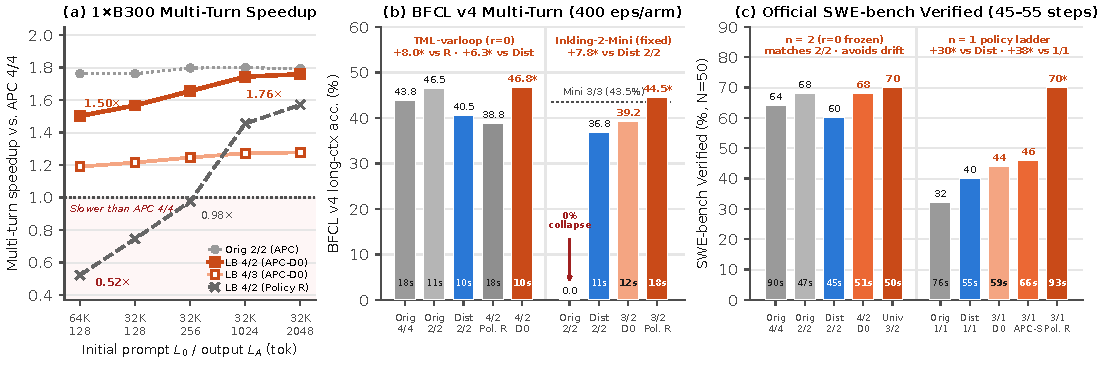
\includegraphics[width=0.93\textwidth]{../figs/fig_multiturn_agentic.pdf}
\caption{\textbf{Multi-turn and agentic serving on 26.4B Inkling-2 in Day-0 vLLM (1$\times$/8$\times$B300; bar base: LLM s/ep).}
Policies: \emph{Pol.~R} = full re-prefill (Policy~I accuracy, no APC); \emph{D0/APC-D0} = turn-0 fold + APC;
\emph{APC-S} = suffix-only fold. (a)~\emph{1$\times$B300 speedup vs.\ APC~4/4 ($L_0{=}32\text{--}64\text{K}, L_U{=}2\text{K}$):}
Pol.~R drops to $0.52$--$0.75\times$ on short outputs ($1.0\times$ at $L_A{\approx}256$), whereas APC-D0 sustains
$1.50$--$1.76\times$ (83.6\% APC). (b)~\emph{BFCL~v4 \texttt{long\_context} (400 eps/arm, 15,200 total):} on
\texttt{TML-varloop}, APC-D0 matches Orig~2/2 (46.8\% vs.\ 46.5\%), flips Pol.~R by $+8.0^\ast$ ($p{=}0.0044, 1.77\times$),
and beats Dist~2/2 by $+6.3^\ast$ ($p{=}0.012$); on fixed-depth Mini, LoopBridge rescues 0\% collapse and Pol.~R beats
Dist~2/2 by $+7.8^\ast$ ($p{=}0.0044$). (c)~\emph{Official SWE-bench Verified (19 arms, 96.4\% APC):} $r{=}0$ Univ~3/2
(70\%, 50~s) and 4/2~D0 (68\%, 51~s) match Orig~2/2 (68\%, 47~s) while avoiding Dist~2/2 drift (60\%); at $n{=}1$,
upgrading $A_{t-1}$ lifts 32\% Orig / 40\% Dist~1/1 to 70\% ($+38^\ast/+30^\ast, p{<}10^{-4}$). Appendix~\ref{app:multiturn}.}
\label{fig:multiturn}
\end{figure*}

\paragraph{Fixed-depth backbones and $n{=}1$: Merged LoRA rescues collapse.}
On fixed-3 \texttt{Inkling-2-Mini}, all unadapted $n{=}2$ setups collapse (Anchored TF~3/2: 2.2\%, 93.2\% trunc.;
Procrustes~3/2: 11.1\% GPQA), and \texttt{TML-d24-varloop} stalls at $n{=}1$ (40.8\%). Pairing the KV bridge with
merged LoRA under locked 24M budgets ($5\times$avg@4; Figure~\ref{fig:inkling_main}b) beats parameter-advantaged tied
distillation on \texttt{Inkling-2-Mini}~3/2 (57.7\% vs.\ 52.0\%, $+5.7^\ast$ / $+9.4^\ast$ long, $4.5\times$ faster
train) and \texttt{TML-varloop}~3/1 (50.0\% vs.\ 44.7\%, $+5.3^\ast$ / $+8.5^\ast$, $3.55\times$ faster; $p{<}10^{-4}$),
where a 3-step ablation ($48.9\to49.7\to50.0$) confirms global-3 KV maps drive $+4.70^\ast$ on 512K MRCR ($p{=}0.017$).
Isolated 1$\times$B300 Day-0 vLLM telemetry confirms $<1\%$ decode overhead ($1.26$--$2.76\times$ pure decode vs.\ 4/4
across $L{=}512$--256K), 96.8--97.9\% PyTorch--vLLM parity, $1.25$--$3.58\times$ async/saturated Poisson ITL speedups,
and 0 preemptions (Table~\ref{tab:vllm_speed}).

\subsection{Multi-Turn and Agentic Serving}
\label{sec:multiturn}

We evaluate all four Section~\ref{sec:mt_method} policies across isolated systems grids and two executable agentic suites
to test directly when multi-turn recomputation offsets decode savings (Figure~\ref{fig:multiturn},
Appendix~\ref{app:multiturn}).

\paragraph{Hardware crossover on 1$\times$B300 multi-turn grids.}
Figure~\ref{fig:multiturn}a confirms that \emph{naive full re-prefill (Policy~R, APC off) fails on long-history,
short-output agents}: at $L_0{=}64\text{K}, L_A{=}128, T{=}8$, recomputing $O(m T^2)$ tokens slows 4/2 to $13.6\text{ s}$
vs.\ $7.1\text{ s}$ for APC~4/4 ($0.52\times$), crossing $1.0\times$ only at $L_A{\approx}256$ ($0.98\times$) before
reaching $1.57\times$ at $L_A{=}2048$. By contrast, \textbf{Policy~APC-D0} (83.6\% APC hit rate, zero dual-KV buffer)
sustains \textbf{$1.50$--$1.76\times$ speedup} over APC~4/4 across \emph{every} workload ($4.72\text{ s}$ at
$64\text{K}/128$, $2.87\times$ faster than Policy~R; $36.7\text{ s}$ vs.\ $64.5\text{ s}$ at $32\text{K}/2048$).
Measured incremental 4-pass prefill TTFT bounds analytical Policy~I at only $43$--$105\text{ ms/turn}$ ($<0.2\%$/turn
of a 64~s trajectory), projecting $1.51$--$1.77\times$ speedups for $+50\%$ global KV slots (Policy~I's dual-KV engine
is unimplemented in vLLM; Table~\ref{tab:mt_systems}).

\begin{table*}[t]
\centering\footnotesize
\setlength\tabcolsep{2.0pt}
\begin{tabular}{@{}lc*{11}{c}@{\hspace{5pt}}c@{}}
\toprule
method & $m/n$ & MMLU & MMLU-P & BBH & ARC-C & HellaSw. & Winogr. & GSM8K & MATH & HE+ & MBPP+ & RULER & Avg. \\
\midrule
\csname @@input\endcsname ../figs/tab_main.tex
\bottomrule
\end{tabular}
\caption{\textbf{LoopBridge beats Original and tied distillation at equal decode loops on dense Ouro-2.6B} (accuracy \%;
shaded: LoopBridge, bold: best/group). \emph{Training-free}: 4 prefill loops (last-loop KV reuse). \emph{Distilled
r16/r80}: tied-loop LoRA KD on the same 48M tokens and 4/4 teacher (r80 matches LoopBridge's 63.3M params). First seed
shown; 3-seed means ($\pm$s.d.): $58.3{\pm}0.1$ (4/1), $68.6{\pm}0.4$ (4/2) vs.\ Distilled r16 $49.6{\pm}0.3$,
$66.1{\pm}0.1$ (r80: $49.2{\pm}0.1$, $65.6{\pm}0.2$).}
\label{tab:main}
\end{table*}

\paragraph{Stateful tool-calling agents: BFCL~v4 Multi-Turn (15,200 episodes).}
Across 19 arms (avg@2 on \texttt{base} and \texttt{long\_context}, 12.5 steps/ep, up to 20K context, 91.5\% APC hit
rate; Figure~\ref{fig:multiturn}b, Table~\ref{tab:bfcl_mt}):
\begin{itemize}
\item On \texttt{TML-d24-varloop}, naive Policy~R hurts both speed and accuracy ($38.8\%$ @ $18.5\text{ s}$ on
\texttt{long\_context} vs.\ $43.8\%$ @ $17.7\text{ s}$ for APC~4/4). \textbf{Policy~APC-D0} with frozen $r{=}0$ KV maps
flips 4/2 to \textbf{46.8\% @ 10.5~s} (preserving Orig~2/2's 46.5\% / 48.3\% avg while flipping Policy~R by $+8.0^\ast$
[$p{=}0.0044, 1.77\times$] and avoiding Distilled~2/2's LoRA drift [$+6.3^\ast, p{=}0.0124$ vs.\ 40.5\%; $1.69\times$
vs.\ APC~4/4]). Under ultra-short \texttt{effort=low} ($\sim$115~tok/step), APC-D0 sweeps every baseline on both splits
(47.0\% avg vs.\ 44.5\% Orig~2/2, 44.0\% APC~4/4 at $1.42$--$1.52\times$, and 42.0\% Policy~R [$+5.0^\ast, p{=}0.0060$]).
\item On fixed-depth \texttt{Inkling-2-Mini}, Original~2/2 collapses to \textbf{0.0\%} (0/800). LoopBridge~3/2 with
APC-D0 rescues it to 49.5\% / 39.2\% (beating Distilled~2/2's 47.8\% / 36.8\% at matched latency), while deep 3-pass KV
bridging over late-turn tool logs (\textbf{Policy~R}, Policy~I accuracy, 17.9~s) lifts \texttt{long\_context} to
\textbf{44.5\%} ($+7.8^\ast$ vs.\ Distilled~2/2, $p{=}0.0044$, exceeding Orig~3/3's 43.5\%).
\end{itemize}

\begin{table*}[t]
\centering\footnotesize
\setlength\tabcolsep{3.8pt}
\begin{minipage}[c]{0.60\textwidth}\centering
\begin{tabular}{@{}lccc@{}}
\toprule
variant (4/1) & KV maps & average & RULER-16K \\
\midrule
\csname @@input\endcsname ../figs/tab_build.tex
\bottomrule
\end{tabular}
\par\smallskip(a) What LoopBridge adds (all $(m,n)$ pairs).
\end{minipage}\hfill
\begin{minipage}[c]{0.38\textwidth}\centering
\begin{tabular}{lcccc}
\toprule
\csname @@input\endcsname ../figs/tab_tokens.tex
\bottomrule
\end{tabular}
\par\smallskip(b) Training tokens (one-cache).

\smallskip
\begin{tabular}{lccc}
\toprule
learning rate & $0.3\times$ & $1\times$ & $3\times$ \\
\midrule
\csname @@input\endcsname ../figs/tab_lr.tex
\bottomrule
\end{tabular}
\par\smallskip(c) Scaled learning-rate schedule.
\end{minipage}
\caption{\textbf{Ouro-2.6B ablations} (11-benchmark average \% unless noted; default shaded). (a) Every row serves all
$(m,n)$ pairs with one adapter; KV maps restore RULER-16K lost by decoder-only LoRA even at matched rank~80 ($+8.9^\ast$).
(b) One-cache keeps a strong lead at 6M tokens (54.8 vs.\ 48M Distilled~1/1's 49.5). (c) Lead persists across
$0.3$--$3\times$ LR.}
\label{tab:ablate}
\end{table*}

\paragraph{Long-horizon coding agents: Official SWE-bench Verified.}
Across 19 arms in isolated zero-Docker \texttt{mini-swe-agent} bash (45--55 steps, 33K--58K ctx, 96.0--96.6\% APC;
Figure~\ref{fig:multiturn}c, Table~\ref{tab:swebench}):
\begin{itemize}
\item \emph{Frozen $r{=}0$ avoids drift ($n{=}2$):} While full-LoRA \texttt{Distilled~2/2} drops to 60.0\%, $r{=}0$
\textbf{Universal~3/2 (APC-D0)} hits \textbf{70.0\%} in \textbf{50.4~s} ($1.78\times$ vs.\ 4/4's 89.7~s; directional
$+10.0, p{=}0.058$ vs.\ Distilled~2/2) and \textbf{LB~4/2~KV} hits 68.0\% under APC-D0 (51.4~s) / APC-S (50.1~s,
$1.79\times$) and 70.0\% under Policy~R---matching \texttt{Orig~2/2} (68.0\%, 47.1~s, $1.90\times$) without LoRA drift.
\item \emph{Causal 4-policy proof ($n{=}1$):} Orig~1/1 drops to 32.0\% (76.0~s) and 24M \texttt{Distilled~1/1} hits
40.0\% (54.7~s, $1.64\times$ vs.\ 4/4). \texttt{LB~3/1} climbs 44.0\% (APC-D0, 58.7~s, $1.53\times$ vs.\ 4/4
[$1.29\times$ vs.\ 1/1]) $\to$ 46.0\% (APC-S, folding $U_t$, 66.2~s) $\to$ \textbf{70.0\%} (Policy~R, 92.7~s
[$0.97\times$], projecting Policy~I speed; $+38.0^\ast$ vs.\ 1/1, $+30.0^\ast$ vs.\ Dist~1/1, $p{<}10^{-4}$), isolating
upgrading $A_{t-1}$ as the $+24$-point mechanism.
\item \emph{Honest fixed-depth boundary:} On fixed-depth \texttt{Inkling-2-Mini}, single-turn \texttt{LB~3/2} (62\%
Pol.~R, 58\% APC-D0 [$p{=}0.032$], 50\% APC-S) trails \texttt{Distilled~2/2} (70\%; Orig~3/3 72\%) because 95\% of the
35K trajectory is unseen dynamic bash output, motivating multi-turn asymmetric KD when decoder LoRA is needed.
\end{itemize}

\subsection{Dense Ouro Backbones and Decision Models}
\label{sec:main}

\paragraph{Main 11-benchmark gains and directional asymmetry.}
On fixed-depth Ouro-2.6B (Table~\ref{tab:main}), naive untying collapses (28.7 at 4/1, 31.0 at 4/2). LoopBridge~4/1
lifts the 11-benchmark average from 44.2 (Original~1/1) to \textbf{58.2}, $+8.7$ ahead of Distilled~1/1 (49.5; 49.3 at
parameter-matched rank~80), improving every benchmark by up to $+23$ points. At 4/2, LoopBridge reaches \textbf{69.1}
($68.6$ over 3 seeds) vs.\ 63.7 Original~2/2 and 66.2 Distilled~2/2 (winning 10/11 tasks, within 2.8 of 4/4 at half the
decode loops). Across all 16 pairs $(m,n)\in\{1..4\}^2$ within one adapter (Figure~\ref{fig:teaser}a;
Appendix~\ref{app:extended}), raising $m$ from 1 to 4 adds $+10$--12 points at every decode depth, while $m{<}n$ hurts on
every pair by 1.9--11.5 points (tied $n/n$ bypasses the adapter for exact Original accuracy).

\paragraph{Depth saturation, batched serving, ablations, and transfer.}
\label{sec:others}
With fixed weights, raising $m$ ($1{\to}4$) adds $+10.7{\pm}0.5$ (3 seeds), saturating in $m\in[2,5]$ before drifting
past $m{=}4$ (16/18 settings; Figure~\ref{fig:depthfull}, Appendix~\ref{app:plateau}). On 800 timed CoT requests
(Appendices~\ref{app:time}, \ref{app:serve}), folded maps keep native speed (27.7 vs.\ 28.3~\mbox{tok/s} at $n{=}1$;
14.3 at 4/2, $2.1\times$ 4/4), scoring 45.0 ($+17.2^\ast$ vs.\ 1/1, $+10.8^\ast$ vs.\ Dist~1/1, $+10.5^\ast$ vs.\
time-matched mix; $+18.5^\ast$/$+11.3^\ast$ at $B{=}32$; Figure~\ref{fig:batched}); on Thinking GSM8K (1,319 items),
batched 4/2 matches 4/4 (94.6 vs.\ 94.2--94.3) in $0.47$--$0.57\times$ time (Figure~\ref{fig:tbatched}). In
Table~\ref{tab:ablate}, dropping the KV bridge cuts 4/1 RULER-16K by 14.9 (8.9 at rank~80), one-cache cuts prompt KV
$n\times$ and lifts 8K decode $1.19$--$1.62\times$ (Figure~\ref{fig:frontier}), and gains hold at 6M tokens,
$0.3$--$3\times$ LR, clean subsets (Appendix~\ref{app:training}), Ouro-1.4B~4/1 (44.5 vs.\ 34.7/40.5,
Table~\ref{tab:main14}), Thinking~4/2 (within 0.8 of 4/4, $+15$ HELMET, Table~\ref{tab:think}), and Lev~\citep{lev}
($m{>}n$ wins all 13 pairs up to $+7.5^\ast$, $m{<}n$ hurts all 13; Figure~\ref{fig:lev}, Table~\ref{tab:lev}).

\section{Conclusion}

Should prefill and decode loop equally? No: parallel prefill is cheap while sequential decode dominates wall time.
Untying them exposes contextual representation shift, which LoopBridge resolves at zero decode overhead via a foldable
prompt KV bridge (sufficient alone on variable-depth MoEs at $n{\ge}2$) plus merged decoder LoRA for fixed-depth
backbones and $n{=}1$. With prefix-cached multi-turn policies, asymmetric loops shift the accuracy--throughput frontier
across dense, sparse-MoE, Thinking, decision, and agentic workloads.

\section*{Limitations}
\label{sec:limits}

Hardware latency is measured on one GPU family (NVIDIA B300) up to batch~32; on single-turn short-output tasks with very
long prompts (128K--256K, $G{=}512$), deeper $m$-pass prefill attenuates end-to-end speedup relative to shallower-$m$
baselines (though 4/3 and 4/2 still beat equal-$m$ Original~4/4 at 262K; Appendix~\ref{app:inkling}). Under
unconstrained single-stream ($B{=}1$) high-effort reasoning on 26.4B models, $n{=}1$ decoders inflate chain-of-thought
length by $1.4$--$1.8\times$, so $n{\ge}2$ dominates $B{=}1$ wall time while $n{=}1$ leads in batched throughput cost.
In multi-turn serving, our vLLM prototype retains $2{+}2m$ global slots (matching Original~$m/m$); achieving $2{+}2n$
memory requires freeing unaligned prefill slots post-fold, whereas exact Policy~I for $n{=}1$ (analytical here and
unimplemented in vLLM; accuracy evaluated via Policy~R) requires dual KV state
($3{+}2m{+}2n$ global slots plus 160--200~MiB SWA/SConv boundary state). Finally, single-turn asymmetric LoRA adapters on
fixed-depth \texttt{Inkling-2-Mini} underperform tied distillation on 40-step SWE-bench bash trajectories (50--62\% vs.\
70\%), motivating multi-turn-aware asymmetric distillation and per-prompt adaptive depth routing as future work.


\FloatBarrier
\begingroup\emergencystretch=3em
\bibliography{references}
\endgroup

\clearpage
\appendix
\renewcommand{\dblfloatpagefraction}{0.65}\renewcommand{\floatpagefraction}{0.65}

\paragraph{Guide to the appendix.} Appendix~\ref{app:time} gives per-request times behind Figures~\ref{fig:time}
and~\ref{fig:batched}, Appendices~\ref{app:plateau} and~\ref{app:depth14} the depth sweeps (Figure~\ref{fig:depthfull}),
and Appendix~\ref{app:extended} per-domain $(m,n)$ charts (Figure~\ref{fig:grid}) and every cell (Table~\ref{tab:alignedcells})
plus Thinking and decision-model results. Appendix~\ref{app:method} gives method details, Appendix~\ref{app:related} extended related
work, and Appendices~\ref{app:training} and~\ref{app:eval} training and evaluation details.
Appendices~\ref{app:models}--\ref{app:inkling} cover other checkpoints, the Thinking model in numbers, batched serving,
design variants, decision models, and our 26.4B sparse-MoE vLLM scale-up; Appendix~\ref{app:multiturn} details our
multi-turn and agentic serving experiments (1$\times$ B300 systems grid, BFCL~v4 Multi-Turn, and official SWE-bench
Verified); and Appendix~\ref{app:repro} lists what is released.
Throughout, \emph{one-cache LoopBridge} refers to the lighter variant in which every decode loop reads the last prefill
loop. In comparison figures, LoopBridge is shown in orange, Original in grey, and Distilled in blue.
Table~\ref{tab:impl} lists the implementation and measurement behind each result.

\begin{table}[h]
\centering\footnotesize
\setlength\tabcolsep{2.5pt}
\begin{tabular}{@{}>{\raggedright\arraybackslash}p{0.33\columnwidth}>{\raggedright\arraybackslash}p{0.31\columnwidth}>{\raggedright\arraybackslash}p{0.29\columnwidth}@{}}
\toprule
result & LoopBridge form & measurement \\
\midrule
Figure~\ref{fig:teaser}a (TPS); Figures~\ref{fig:batched} (B=1), \ref{fig:budgetfull}; Table~\ref{tab:time} & per-loop caches, maps folded in (merged decode LoRA) & batch 1, 800 timed requests ($n{=}3$: 400) \\
\addlinespace[4pt]
Figures~\ref{fig:batched} (B=8, 32), \ref{fig:tbatched}; Tables~\ref{tab:batched}, \ref{tab:tbatched} & per-loop caches, maps folded in (merged decode LoRA) & continuous batching, wall time \\
\addlinespace[4pt]
Tables~\ref{tab:ablate}b, \ref{tab:models}; Figure~\ref{fig:frontier}; last row of Table~\ref{tab:ablate}a; Appendix~\ref{app:serve} (8K decode) \& \ref{app:variants} (key maps) & one shared cache & accuracy; decode microbenchmark \\
\addlinespace[4pt]
Figure~\ref{fig:teaser}b; Figures~\ref{fig:inkling_main}, \ref{fig:inkling_speed}; Tables~\ref{tab:varloop}--\ref{tab:vllm_speed} (Appendix~\ref{app:inkling}) & folded NoPE global-3 KV maps ($r{=}0$ KV-Only or merged decode LoRA) in vLLM & 5 official benchmarks (256K--1M, avg@4 \& avg@1); 1$\times$ B300 SSE timing \\
\addlinespace[4pt]
Figure~\ref{fig:multiturn}; Tables~\ref{tab:mt_systems}--\ref{tab:swebench} (Appendix~\ref{app:multiturn}) & Day-0 vLLM multi-turn policies (APC-D0, APC-S, Policy~R) & 1$\times$ B300 8-scenario grid; BFCL~v4 (15,200 eps); SWE-bench Verified ($N{=}50$) \\
\addlinespace[4pt]
all other LoopBridge results (and Appendix~\ref{app:time}'s 45.4 check) & per-loop caches, maps folded at prefill (unmerged LoRA; 45.4 uses merged LoRA with per-step maps) & accuracy \\
\bottomrule
\end{tabular}
\caption{\textbf{Implementation behind each result.} In exact arithmetic, folded and per-step per-loop forms compute the
same function (Section~\ref{sec:method}). One-cache LoopBridge is a separately trained variant.}
\label{tab:impl}
\end{table}

\section{Per-Request Time}
\label{app:time}

\begin{figure}[t]
\centering
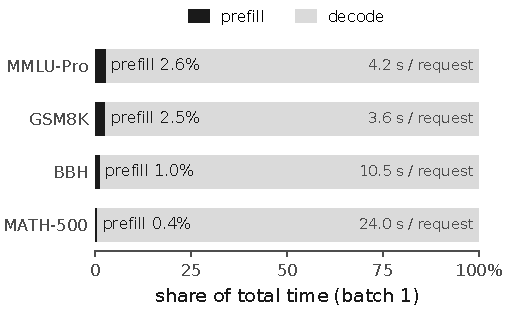
\includegraphics[width=\columnwidth]{../figs/fig_time.pdf}
\caption{\textbf{At batch 1, prefill takes almost no time.} Share of the total time over 200 requests per task spent reading the
prompt (prefill, black) and writing the answer (decode, grey). We test released Ouro-2.6B at one loop (Original~1/1),
batch~1, on one B300 GPU.}
\label{fig:time}
\end{figure}

Table~\ref{tab:time} gives the per-request distributions behind Figure~\ref{fig:time}. We test every configuration on the
same 200 requests per task (batch~1, one B300, greedy). The table reports medians and 90th percentiles of output length,
time per request, and prefill share. At the 90th percentile, prefill share is under 2\% on MATH-500 and at most 8\% on
GSM8K and BBH, but reaches 6--19\% on MMLU-Pro, where many answers are short. Time per request follows output length.
Some outputs run on to the length limit (2,048 tokens on MMLU-Pro) without giving an answer, most often at one decode
loop: on MMLU-Pro this happens for 29 of 200 requests with LoopBridge~4/1 and 15 with Distilled~1/1, against 4 with
Original~1/1. These outputs take most of MMLU-Pro's wall time and explain most of LoopBridge~4/1's extra mean time per
request (Section~\ref{sec:main}, Figure~\ref{fig:budgetfull}).

Each reported time is the mean of two passes over the same requests in opposite orders on an idle machine; both passes
produce identical answers. Folding the maps changes floating-point rounding, so greedy answers can differ slightly from
per-step maps: on the four tasks, LoopBridge~4/1 scores 45.0 with folded maps and 45.4 with per-step maps.

\begin{table*}[h]
\centering\small
\setlength\tabcolsep{4.5pt}
\begin{tabular}{@{}llrrrrrrrr@{}}
\toprule
 & & \multicolumn{3}{c}{tokens} & \multicolumn{2}{c}{s / request} & \multicolumn{3}{c}{prefill share (\%)} \\
\cmidrule(lr){3-5}\cmidrule(lr){6-7}\cmidrule(l){8-10}
task & configuration & in med. & out med. & out p90 & med. & p90 & med. & p90 & total \\
\midrule
\csname @@input\endcsname ../figs/tab_time.tex
\bottomrule
\end{tabular}
\caption{\textbf{Per-request time, Ouro-2.6B.} Values are medians unless marked p90 (90th percentile); LoopBridge rows
shaded. Prefill share is prefill time over total time per request; ``total'' is summed prefill time over summed wall
time across all 200 requests (Figure~\ref{fig:time}, Section~\ref{sec:time}). Long answers dominate ``total'', so it is
lower than the median on MMLU-Pro, where many answers are short.}
\label{tab:time}
\end{table*}

\begin{figure}[h]
\centering
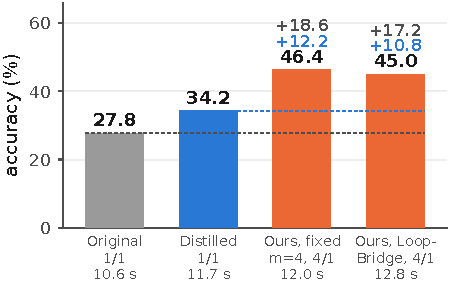
\includegraphics[width=\columnwidth]{../figs/fig_sametime.pdf}
\caption{\textbf{Paired gains at one decode loop.} Ouro-2.6B, the 800 timed requests of Figure~\ref{fig:batched}
(batch~1, one B300, mean of two passes): mean accuracy, with mean time per request under each bar. Grey and blue
numbers: gain over Original~1/1 and over Distilled~1/1 on the same requests (intervals in Section~\ref{sec:main}).}
\label{fig:budgetfull}
\end{figure}


\section{Where the Gain Stops}
\label{app:plateau}

We split each benchmark into two halves by a hash of the item id. On the first half, the stopping depth $m^\ast$ is the
first prefill depth that none of the next three evaluated depths beats by more than 0.5 points. Table~\ref{tab:plateau}
shows held-out accuracy at $m=1$ and at $m^\ast$ on the second half. Settings where accuracy still rises at the largest
evaluated depth (or where too few larger depths were run) have no stopping depth and are omitted: for the main adapter
($m\le4$), MMLU, MMLU-Pro, BBH, and ARC-Challenge at $n=1$, MMLU-Pro and ARC-Challenge at $n=2$, and HellaSwag and
Winogrande at both; for the $m\le16$ adapter, MMLU-Pro and ARC-Challenge at $n=2$ (HellaSwag and Winogrande were not run
for $m\le16$; Table~\ref{tab:depthwide}). Over three training seeds of the $m\le16$ adapter, the stopping depth lies
between two and five loops in 13 of 14 settings that stop in every seed.

\begin{figure*}[t]
\centering
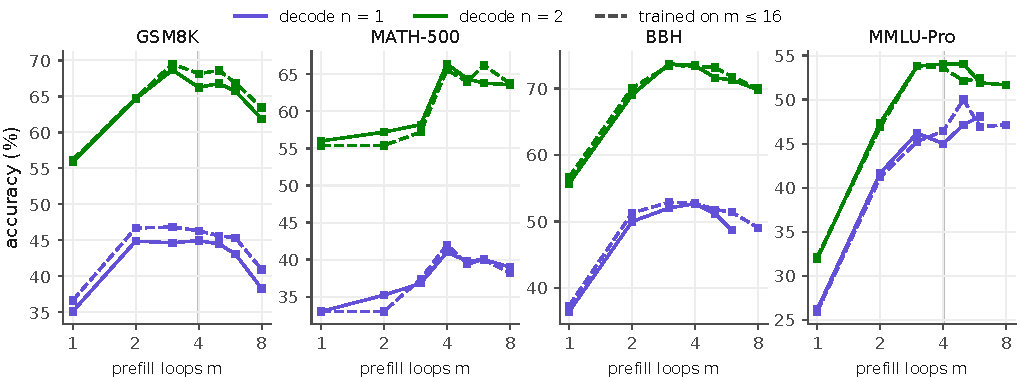
\includegraphics[width=\textwidth]{../figs/fig_depth.pdf}
\caption{\textbf{More prefill loops on the timed tasks.} Ouro-2.6B, same weights at every $m$; decode $n=1$ (violet)
and $n=2$ (green). Accuracy on the evaluation sets of Appendix~\ref{app:eval}; solid: adapter trained on $m\le4$
(up to $m=6$ on BBH and MMLU-Pro at $n=1$), dashed: adapter trained on $m\in\{1,2,3,4,6,8,12,16\}$ (shown for
$m\le8$, up to $m=6$ on MMLU-Pro at $n=2$; $m=12,16$ in Table~\ref{tab:depthwide}); vertical grey line: $m=4$.}
\label{fig:depthfull}
\end{figure*}

\paragraph{Training the prefill as well.} In the adapters above, the prefill loops stay frozen. To test whether gains stop
only because prefill was never trained for deeper looping, we train two adapters differing in only one way: both train on
$m\in\{1,2,3,4,6,8\}$ and $n\le4$ with training prompts truncated to their last 2,048 tokens so backpropagating through
eight prefill loops fits in memory (evaluation prompts are never truncated). One keeps prefill frozen; the other adds
rank-16 LoRA to the prefill attention (Table~\ref{tab:prefilltrn}, seed~1). Training prefill does not make the gain stop
later: across the 14 settings where both adapters stop, the trained-prefill adapter stops later in 2, at the same depth
in 6, and earlier in 6 (both stop at two to five loops in all 14). Across three seeds, no setting stops later with
trained prefill in every seed. Training prefill mainly helps long prompts: on RULER-16K, it raises peak accuracy from
63.7 to 66.0 at $n=1$ and from 75.2 to 81.0 at $n=2$.

\begin{table}[t]
\centering\footnotesize
\setlength\tabcolsep{3.2pt}
\begin{tabular}{@{}llrrrr@{}}
\toprule
 & & & & \multicolumn{2}{c}{acc.\ (\%)} \\
\cmidrule(l){5-6}
range & benchmark & $n$ & $m^\ast$ & $m{=}1$ & $m{=}m^\ast$ \\
\midrule
\csname @@input\endcsname ../figs/tab_plateau.tex
\bottomrule
\end{tabular}
\caption{\textbf{Stopping depth of the prefill gain.} Held-out accuracy (\%) at $m=1$ and stopping depth $m^\ast$;
``$m\le4$'' is the default adapter (extrapolating past 4) and ``$m\le16$'' is trained on
$m\in\{1,2,3,4,6,8,12,16\}$.}
\label{tab:plateau}
\end{table}

\begin{table*}[t]
\centering\footnotesize
\setlength{\tabcolsep}{4pt}
\begin{tabular}{@{}lrlrrrrrrrrrr@{}}
\toprule
benchmark & $n$ & prefill & $m{=}1$ & 2 & 3 & 4 & 5 & 6 & 8 & 12 & 16 & $m^\ast$ \\
\midrule
\csname @@input\endcsname ../figs/tab_prefilltrn.tex
\bottomrule
\end{tabular}
\caption{\textbf{Training the prefill loops as well.} Accuracy (\%) against prefill loops $m$ for two adapters trained
identically on $m\le8$ with prompts cut to 2,048 tokens, one with prefill frozen and one with LoRA on prefill attention;
shared items; best printed $m$ in bold. $m^\ast$: stopping depth on the first half as in Table~\ref{tab:plateau}
(``--'' in $m^\ast$: omitted where either arm has no stopping depth; ``--'' in an $m$ column: not evaluated).}
\label{tab:prefilltrn}
\end{table*}

\begin{table*}[t]
\centering\small
\begin{tabular}{@{}lrrrrrrrrrr@{}}
\toprule
benchmark & $n$ & $m{=}1$ & 2 & 3 & 4 & 5 & 6 & 8 & 12 & 16 \\
\midrule
\csname @@input\endcsname ../figs/tab_depthwide.tex
\bottomrule
\end{tabular}
\caption{\textbf{Prefill depth for the adapter trained up to 16 loops} (Figure~\ref{fig:depthfull}). Ouro-2.6B, accuracy (\%)
against prefill loops $m$ at decode $n$, same weights for every $m$, on the evaluation sets of Table~\ref{tab:main}
(nine of its 11 benchmarks; HellaSwag and Winogrande not run); best $m$ of each row in bold; ``--'': not evaluated.}
\label{tab:depthwide}
\end{table*}

\section{Prefill Depth on Ouro-1.4B}
\label{app:depth14}

Table~\ref{tab:depth14} repeats the sweep of Appendix~\ref{app:plateau} (Figure~\ref{fig:depthfull}) on Ouro-1.4B with LoopBridge (trained on
$m,n\le4$), using the same benchmarks and protocol (full MMLU and GSM8K; Table~\ref{tab:main14} uses subsets).

\begin{table}[t]
\centering\small
\begin{tabular}{@{}lrrrrr@{}}
\toprule
benchmark & $n$ & $m{=}1$ & 2 & 3 & 4 \\
\midrule
\csname @@input\endcsname ../figs/tab_depth14.tex
\bottomrule
\end{tabular}
\caption{\textbf{Prefill depth on Ouro-1.4B.} Accuracy (\%) against prefill loops $m$ at decode $n$ over the adapter's
training range $m\le4$; best $m$ of each row in bold. BBH at $n=1$: see the format note under Table~\ref{tab:main14}.}
\label{tab:depth14}
\end{table}

\section{Additional Results}
\label{app:extended}

Figure~\ref{fig:grid} breaks down Figure~\ref{fig:teaser}a across four representative domains (knowledge, reasoning,
math, and 16K retrieval), and Table~\ref{tab:alignedcells} gives every $(m,n)$ cell across all 11 Ouro-2.6B benchmarks.

\begin{figure*}[t]
\centering
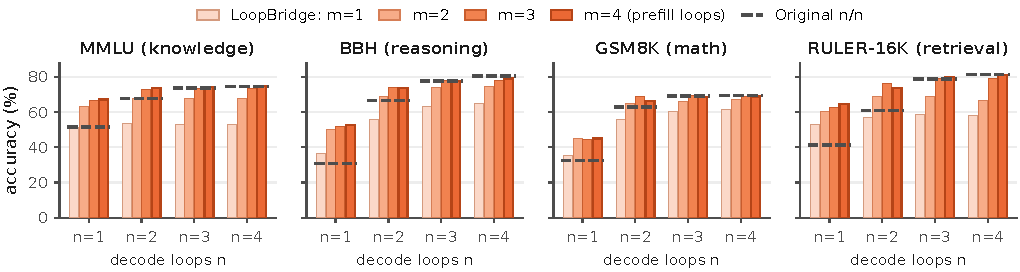
\includegraphics[width=0.96\textwidth]{../figs/fig_taskmap_domains.pdf}
\caption{\textbf{Per-domain $(m,n)$ breakdown across knowledge, reasoning, math, and 16K retrieval} (Ouro-2.6B, all 16
pairs $m,n\in\{1..4\}$ vs.\ Original~$n/n$ dashed; 11-benchmark average in Figure~\ref{fig:teaser}a and every cell in
Table~\ref{tab:alignedcells}). Knowledge (MMLU) and retrieval (RULER-16K) depend heavily on prefill depth $m$, while
multi-step reasoning (BBH, GSM8K) also benefits strongly from decode depth $n$.}
\label{fig:grid}
\end{figure*}

\begin{figure*}[t]
\centering
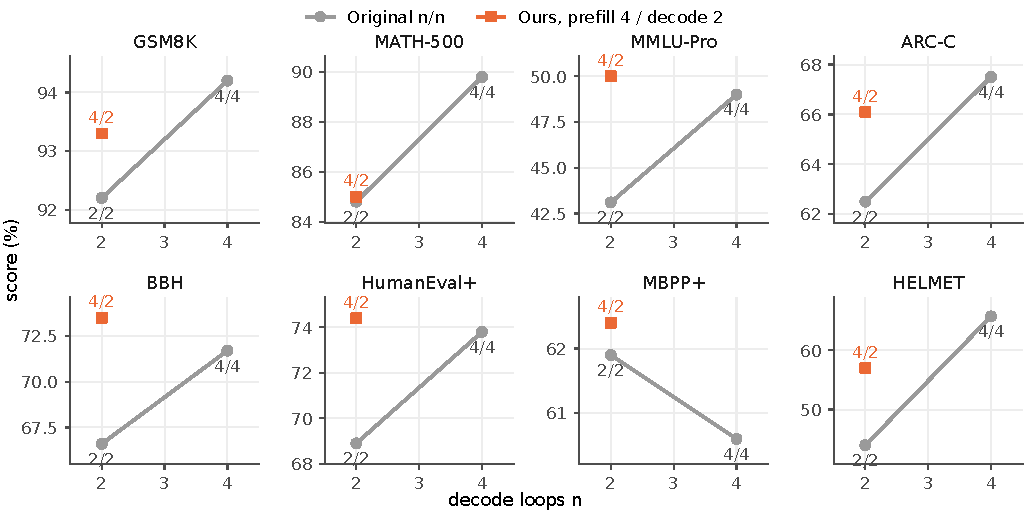
\includegraphics[width=0.94\textwidth]{../figs/fig_equal.pdf}
\caption{\textbf{On a Thinking model, four prefill loops bring two decode loops close to four.}
Ouro-2.6B-Thinking, score (\%) against decode loops $n$. Orange: LoopBridge~4/2; grey: Original~2/2 and 4/4; blue:
Distilled~2/2 (drawn just left of $n=2$). Same items for all four in each panel; HELMET is averaged over its categories.
Over three training seeds, LoopBridge~4/2 averages $1.1\pm0.3$ points below Original~4/4. Table~\ref{tab:think} gives
every score, paired intervals, and the same adapter at 2/2.}
\label{fig:equal}
\end{figure*}


\begin{table*}[t]
\centering\footnotesize
\setlength\tabcolsep{2.4pt}
\begin{tabular}{@{}l*{11}{c}@{\hspace{5pt}}c@{}}
\toprule
\csname @@input\endcsname ../figs/tab_aligned.tex
\bottomrule
\end{tabular}
\caption{\textbf{Every prefill/decode cell of LoopBridge.} Ouro-2.6B, accuracy (\%) of Original~$n/n$ and LoopBridge~$m/n$
for all 16 pairs $m,n\in\{1,\dots,4\}$ on the benchmarks of Table~\ref{tab:main}, plus the 11-benchmark average. Each
column intersects full Original~4/4 runs with the Section~\ref{sec:setup} subsets (Figure~\ref{fig:grid}); bold: best $m$
for LoopBridge at each $n$. At tied 3/3 and 4/4, serving can bypass the adapter to run Original directly.}
\label{tab:alignedcells}
\end{table*}


\subsection{Ouro-2.6B-Thinking at 4/2}
\label{sec:thinking42}

Figure~\ref{fig:equal} shows Ouro-2.6B-Thinking on each benchmark at 4/2. With the same decode loops as \nat{2},
LoopBridge~4/2 scores higher on six of eight benchmarks---by 15 points on HELMET and 8 on MMLU-Pro and BBH---and stays
within 0.5 points on MATH-500 and MBPP+. Against \nat{4}, which decodes with twice the loops, it is within two points or
better on six of eight (trailing on MATH-500 by 5.2 and HELMET by 6.8). Against Distilled~2/2, trained on the same data,
it is higher on six of eight and within 0.2 points on MATH-500 and MBPP+ (Table~\ref{tab:think}). The gain comes from
prefill depth: at 2/2, the same adapter scores lower than at 4/2 on all eight benchmarks, by up to 9.6 points on MMLU-Pro.

\subsection{Looped decision models: both directions}
\label{sec:lev}

Untying is not specific to generation. Lev~\citep{lev} turns looped language models into decision models that read a
context and score question options with a learned head after every loop, without generating text. We prefill the context
with $m$ loops, and each of the $n$ decision loops attends to the last prefill loop's KV. We continue training Lev's own
LoRA and scoring head once for every $m$; the control continues training the same weights on the same data for the same
updates with Lev's Original~$n/n$ forward (Appendix~\ref{app:lev}).

For $m\ne n$, the sign of $m-n$ determines whether untying helps or hurts (Figure~\ref{fig:lev}, Table~\ref{tab:lev}).
With more context than decision loops, the model beats the control on all 13 $m>n$ pairs (significantly on 12), peaking
at one decision loop: $+5.3$\ci{3.4}{7.2} on Lev-1.4B, $+7.5$\ci{5.7}{9.5} on Lev-2.6B, and $+4.4$\ci{2.8}{6.1} on Lev-3B.
In contrast, with fewer context than decision loops, the model trails the control on all 13 $m<n$ pairs (significantly on
11), dropping up to $-13.0$\ci{-14.7}{-11.3} (Lev-2.6B, $m=1, n=4$). The $m<n$ drop replicates over four training seeds
(below the control on all 13 pairs in every seed, 10 significant in every seed). The $m>n$ gain at full context depth
also replicates over four seeds and against a control trained twice as long (Appendix~\ref{app:lev}). As with language
models (Figure~\ref{fig:grid}), context benefits from many loops while the decision can use few.

\section{Method Details}
\label{app:method}

We describe LoopBridge for Ouro (Figure~\ref{fig:method}).

\begin{figure*}[t]
\centering
\rule{\textwidth}{0.4pt}\\[-2pt]
\begin{minipage}[t]{0.495\textwidth}
\begin{lstlisting}
# blocks: frozen block (L layers); m/n: prefill/decode
# c[k][l] = 1+a+1j*b per RoPE pair (init: 1, / KV head)
# W[k][l] = I+delta per KV head (init: I); LoRA: decode

def prefill(prompt, m):            # excl. last token
    h = embed(prompt)
    for j in range(m):
        for l in range(L):
            h, K[j][l], V[j][l] = blocks[l](h)
    return K, V

def attend(q, K, V, kv_ans, c, W): # layer l, loop k
    qc = complex_mul(q, c.conj())  # key scale on query
    o_p, lse_p = flash_attn(qc, K, V)
    o_p = o_p @ W.T                # linear value map
    o_a, lse_a = flash_attn(q, *kv_ans, causal=True)
    g = torch.sigmoid(lse_p - lse_a)
    return g * o_p + (1 - g) * o_a
\end{lstlisting}
\end{minipage}\hfill
\begin{minipage}[t]{0.485\textwidth}
\begin{lstlisting}
def decode(token, K, V, m, n): # last prompt, then ans
    h = embed(token)
    for k in range(n):
        # per-loop caches; one-cache: j = m - 1
        j = max(m - n + k, 0)
        for l in range(L):
            h = blocks[l](h, attn=lambda q, kv: attend(
                    q, K[j][l], V[j][l], kv,
                    c[k][l], W[k][l]))
    return lm_head(h)

# training: random (m, n), teacher = Original 4/4
m, n = torch.randint(1, 5, (2,)).tolist()
with torch.no_grad():
    t = original(x, loops=4)       # frozen teacher
s = model(x, prefill=m, decode=n)  # LoRA + KV maps
kl = kl_div(s.log_softmax(-1), t.log_softmax(-1),
            log_target=True, reduction="none").sum(-1)
loss = kl[ans].sum() / (ans.sum() - len(x)) # App. G
\end{lstlisting}
\end{minipage}\\[-1pt]
\rule{\textwidth}{0.4pt}
\caption{\textbf{LoopBridge in PyTorch-style pseudocode.} Decode loop $k$ reads prefill loop $\max(m-n+k,0)$ (0-indexed;
one-cache LoopBridge uses $j=m-1$) through its key scale (on the query) and value map (on the prompt attention output),
merging prompt and answer attention exactly via their log-sum-exps. In training, \texttt{ans} masks answer positions and
\texttt{ans.sum() - len(x)} normalises by $\sum_i(|a_i|-1)$ (Appendix~\ref{app:training}).}
\label{alg:loopbridge}
\end{figure*}

\paragraph{Prefill and decode.} LoopBridge~$m/n$ prefills the prompt with $m$ loops and decodes every answer token with
$n$ loops, whereas Original~$n/n$ is the unmodified model. The frozen backbone runs $m$ loops over the prompt up to its
penultimate token, and the final prompt token runs through the $n$ decode loops to emit the first answer token
(Figure~\ref{alg:loopbridge}). With per-loop caches (default LoopBridge), we keep one prompt cache per decode loop and
decode loop $k$ reads prefill loop $\max(m-n+k,1)$ through its own map, recovering Original~$n/n$'s loop pairing when
$m=n$ and matching Original~$n/n$'s KV memory. In one-cache LoopBridge, trained identically, every decode loop reads the last
prefill loop's cache, storing the prompt once at a small accuracy cost (mostly on long-context retrieval). The decoder
adds a single rank-16 LoRA~\citep{lora} ($\alpha=16$, shared across decode loops) on the query, key, value, and output
projections, active only when decoding.

\paragraph{RoPE-commuting maps.} Decode loop $k$ reads the prompt KV cache through a map per (loop, layer, KV head;
broadcast across query heads in GQA). The key map is one complex scale $c_j$ per rotary frequency pair $j$~\citep{rope}.
Viewing split-half key coordinates $(k_j,k_{j+D/2})$ as a 2-D vector, $c_j=r\,e^{i\phi}$ scales by $r$ and rotates by $\phi$.
Writing a key pair rotated for position $s$ as $\tilde k_j = e^{is\theta_j}k_j$, scaling commutes with rotation:
$c_j\tilde k_j = e^{is\theta_j}(c_jk_j)$. Because $\mathrm{Re}\langle q_j, c_j\tilde k_j\rangle = \mathrm{Re}\langle
\bar c_jq_j, \tilde k_j\rangle$, the per-step form applies the map to the query without rewriting the stored cache. (The
timed form of Section~\ref{sec:method} instead folds both maps into the cache once at prefill.) The value map is a full
linear map $W_k$ per KV head. Because attention is linear in values ($\sum_i a_iW_kv_i = W_k\sum_i a_iv_i$), $W_k$ is
applied once to the prompt attention output. Prompt and generated tokens share one softmax: two attention calls produce
outputs $o_P, o_A$ and log-sum-exps $\lambda_P, \lambda_A$, merged as $g\,o_P+(1-g)\,o_A$ with
$g=\sigma(\lambda_P-\lambda_A)$ (the blockwise softmax of FlashAttention~\citep{flashattn,flashattn2}). In one-cache
LoopBridge, prompt KV is stored once for any $n$, so with $b$ bytes of KV per token and loop, an $\ell$-token prompt,
and $t$ answer tokens, total KV is $b(\ell+n\,t)$ instead of $b\,n(\ell+t)$. Applying maps per step equals folding them
into per-loop caches in exact arithmetic: in bfloat16 all 512 greedy tokens we checked agree, though over full answers
rounding still alters a few (Appendix~\ref{app:time}).

\paragraph{What the maps do.} The maps matter for long prompts. For LoopBridge, the same training with maps frozen at the
identity moves ten of 11 benchmarks by at most 2.8 points at 4/1, but lowers RULER-16K from 64.7 to 49.8
(Table~\ref{tab:ablate}a).

\paragraph{Baseline learning rate.} The distilled baselines use LoopBridge's learning-rate schedule (and $\alpha=r$, unit
scaling, for all LoRA ranks $r\in\{4,16,64,80\}$). Scaling the whole schedule by $0.3\times$ or $3\times$ gives
11-benchmark averages of 49.4 and 49.4 for Distilled~1/1 (49.5 at default) and 65.7 and 65.5 for Distilled~2/2 (66.2 at
default). At rank 80 with $3\times$ learning rate, Distilled~1/1 and 2/2 reach 48.4 and 65.4 (49.3 and 65.5 at default;
shifting Distilled by at most 0.7 at rank 16 and 0.9 at rank 80). None comes close to LoopBridge at 4/1 or 4/2 (58.2 and
69.1). Trained at $0.3\times$ and $3\times$ its learning rate, LoopBridge averages 56.8 and 59.0 at 4/1 and 68.4 and 69.3
at 4/2. At each decode depth, its weakest setting stays well above the strongest distilled baseline. We report both
methods at the default rate.

\paragraph{Training.} We distil LoopBridge~\citep{kd} by minimising $\mathrm{KL}(\text{teacher}\,\|\,\text{student})$
over answer positions, with Original~4/4 as teacher. Training uses 48M answer tokens of reasoning traces, instruction
data, long-context data, and web text. One $(m,n)$ pair is sampled per micro-batch, so one set of parameters (63.3M,
2.4\% of Ouro-2.6B) serves all 16 pairs. Details are in Appendix~\ref{app:training}.


\section{Extended Related Work}
\label{app:related}


\paragraph{Looped and elastic depth.} Weight-tied depth recurrence goes back to Universal Transformers and cross-layer
sharing~\citep{ut,albert}. Looped transformers are computationally universal~\citep{giannou2023looped}, can simulate chain-of-thought
steps in latent space~\citep{saunshi2025latent}, and generalise in length with adaptive step
counts~\citep{loopedlengthgen}. Continuous latent reasoning~\citep{coconut} instead feeds the last hidden
state back as the next input embedding. Relaxed Recursive Transformers~\citep{relaxedrecursive} convert pretrained models into looped
models with per-loop LoRA. Mixture-of-Recursions~\citep{mor} and Huginn~\citep{huginn} route or scale the loop count.
Accordion~\citep{accordion} and Elastic Latent Recurrence~\citep{elr} train one model for several depth budgets. ELR
finds that keeping only the last loop's KV retains most of the gain, and Dory1.0-4B~\citep{dory} caches only the last
loop's KV as well. The Parallel Loop Transformer~\citep{plt}, LoopCoder-v2~\citep{loopcoder2}, and shared-memory looped
transformers~\citep{sharedmem} let later loops read the first loop's KV plus a short local window. All of these models
run the same number of loops for prefill and decode. Ouro~\citep{ouro} reports that generated tokens can keep
only the last loop's KV with almost no loss, but that reusing KV caches during prefill costs more than 10 GSM8K
points. LoopBridge is trained to read prompt KV across
loops. FlashLoop~\citep{flashloop} speeds up looped models without training. It uses token-sparse loop updates, sparse
attention, and KV-residual quantisation.

\paragraph{Depth per phase and per token.} Halting~\citep{act,pondernet}, token-level early
exit~\citep{deebert,depthadaptive,calm,layerskip,skipdecode}, and token routing~\citep{mod} spend depth per token.
CALM must also fill the skipped layers' KV for later tokens. Our maps solve this problem per loop. Speculative
decoding~\citep{specdecoding,specsampling} pairs a cheap drafter with a deep verifier. Pause tokens add compute at
prompt positions~\citep{pausetokens}. Deep-encoder/shallow-decoder models~\citep{deepshallow,llm2slm} and
Tandem Transformers~\citep{tandem} spend more capacity on the prompt across separate networks. BridgeKV~\citep{bridgekv},
concurrent with our work, prefills with a large model and decodes with a small model of the same family. It translates the
prompt KV cache between them with a learned module, trained while both models stay frozen (an optional second stage
adds LoRA to the small model). LoopBridge maps the cache between loops of one model instead. In
contrast, SwiftKV~\citep{swiftkv} skips later layers for prompt tokens. Continuous Depth Batching~\citep{cdb} prefills
at full depth, exits early during decode, and studies caches shared across depths. LoopDuet~\citep{loopduet},
concurrent with our work, sets separate prefill and decode loop counts for Huginn and recurrent OLMo-2 without training,
with prefill no deeper than decode. Huginn was trained with random loop counts, whereas Ouro was trained with a
fixed number of loops (four in its later stages) and fails without an adapter when untied (Table~\ref{tab:main}). Position-Aware Depth Decay~\citep{padd} skips
more layers for later tokens. OverFill~\citep{overfill} decodes with a width-pruned model. Fixed Points
Part~II~\citep{fixedpoints2} distils a light prefill network. POP~\citep{pop}, SPEED~\citep{speed}, and
SEED~\citep{seedemit} prefill with less computation than they decode. Decode-Branch Transformers~\citep{decodebranch},
PHD~\citep{phd}, and State-Prediction Separation~\citep{sps} add decode-side computation. Serving systems already run
the two phases on separate hardware~\citep{distserve,splitwise,mooncake} or co-schedule them~\citep{sarathiserve} over
paged KV memory~\citep{vllm}. Untying the loops lets each phase also use its own depth. We vary prefill and decode
loops independently within one adapter and measure what each buys.

\paragraph{Asymmetric KV producers and consumers.} YOCO~\citep{yoco} has a self-decoder produce one global KV cache
that a cross-decoder reads. YOCO-U~\citep{yocou} loops the self-decoder. Its global KV cache does not grow with the
loop count, but every token still runs the loops. KITE~\citep{kite} expands a checkpoint into two towers so that bulk
prefill runs only the KV-producing tower. These architectures are built for the split. We instead adapt an existing
looped model after pretraining and choose the prefill loops $m$ and decode loops $n$ at inference.

\paragraph{Sharing and transferring state.} KV is shared across heads~\citep{mqa,gqa} and layers~\citep{cla,mlkv}. It
is also evicted or compressed per token~\citep{streamingllm,h2o,snapkv,pyramidkv}. Both approaches are orthogonal to
our per-loop reads and can be combined with them. MELT~\citep{melt} post-trains Ouro to keep one gated KV cache per
layer shared by all loops, plus a sliding window over the last generated tokens. This decouples memory from depth, but it does not separate prefill from decode loops or measure which depths a task needs. Looped Latent Attention~\citep{lla}
compresses KV across loops, while BeNice!\@~\citep{benice} and LSTM-style looped transformers~\citep{lstmloop} share the
KV cache.
PLatour~\citep{platour} injects a larger model's prefill states into a smaller decoder. Cache-to-Cache~\citep{c2c},
HeteroFold~\citep{heterofold}, Swarm Telepathy~\citep{swat}, and CacheLink~\citep{cachelink} transfer KV between
models, while Plato's Key~\citep{platoskey} shows that a closed-form orthogonal rotation and global scale transfer
single-token factual keys across frozen LLMs and unlock 18\% of a recipient's ``dark memories'' (facts stored in weights
yet missed without a better key). BellowsKV~\citep{bellows} shares one latent across adjacent layers. Like CacheLink, we
train our maps through the decoder's output, but within one looped model across loop depths rather than across distinct
models: tokens, layers, and positions align natively, so RoPE-commuting key scales (Ouro) or near-isometric global-3
cross-pass maps (Inkling) scale representation alignment to 256K--1M reasoning and real Day-0 vLLM speedups
(Appendix~\ref{app:inkling}). For hybrid attention / linear-recurrence models~\citep{gdn,hymba}, state-swap interventions~\citep{afendulev}
and LatentPort~\citep{latentport} study the two kinds of state.


\section{Training Details}
\label{app:training}

\paragraph{Adapter.} We add a rank-16 LoRA ($\alpha=16$, no dropout) on the query, key, value, and output
projections, active only when decoding. For each (decode loop, layer, KV head), we apply a complex scale to each
rotary frequency pair on keys and a full $D\times D$ value map ($D=128$, head dimension). Both are initialised to the
identity. With a frozen backbone, this adds 63,307,776 trainable parameters for Ouro-2.6B, 12,582,912 of them in the
decoder LoRA.

\paragraph{Objective and data.} The training loss is $\mathrm{KL}(\text{teacher}\,\|\,\text{student})$ summed over
answer positions. We normalise it by $\sum_i(|a_i|-1)$ over the answers $a_i$ of the global batch (one less than the
supervised positions per answer, matching how the released checkpoints were trained). The teacher is Original~4/4 with
the same weights. We sample one pair $(m,n)$ per micro-batch. Training uses 48M answer tokens: OpenThoughts-114k
reasoning traces~\citep{openthoughts} 45\%, T{\"u}lu~3 SFT responses~\citep{tulu3} 40\%, LongAlpaca-12k long-context
answers~\citep{longlora} 5\%, and FineWeb-Edu windows~\citep{fineweb} 10\% (fractions of answer tokens). Prompts reach
up to 7,680 tokens, and answers up to 1,024. The token budget counts $|a|-1$ positions per answer $a$ for LoopBridge and
the distilled baselines alike. Base models see a plain ``User: \ldots\ Assistant:'' format; Thinking models see the same
samples in their chat template. We did not deliberately include benchmark data, and we did not decontaminate the
training corpora. An audit afterwards (\path{ouro/scripts/overlap_audit.py}) finds a 13-token span shared with the
training data in 187 of 542 code prompts (HumanEval+ and MBPP+), 101 of 500 MATH-500 questions, 106 of 14,042 MMLU, 75
of 6,511 BBH, 24 of 1,400 MMLU-Pro, and at most 3 items of each other audited benchmark (GSM8K, ARC-Challenge, HellaSwag,
Winogrande). Items whose extracted question text is unavailable or shorter than 13 tokens cannot be assessed (2,696 MMLU,
296 HellaSwag, 254 BBH, 247 ARC-Challenge, 194 MMLU-Pro, at most 4 elsewhere) and are kept. RULER-16K and HELMET are
synthetic or long-document and not audited. While overlap can inflate raw student-vs-Original scores on code and
MATH-500, it cannot explain gains over Distilled~$n/n$ (trained on the same data) or within-adapter $m=4$ vs.\ $m=1$
gains (same weights). Without overlapping items, LoopBridge~4/1 stays significantly above Distilled~1/1
(Table~\ref{tab:main}) on MMLU ($+14.3$), MMLU-Pro ($+18.2$), BBH ($+12.4$), GSM8K ($+4.6$), MATH-500 ($+8.0$),
HumanEval+ ($+10.0$ on 70 remaining problems), and MBPP+ ($+5.3$); at 4/2, it stays significantly above Distilled~2/2 on
MMLU ($+6.3$), MMLU-Pro ($+7.7$), BBH ($+2.6$), and MATH-500 ($+9.0$), while tying MBPP+ ($+0.4$, $n{=}285$) and
trailing on HumanEval+ ($-2.9$, $n{=}70$) and GSM8K ($-3.3$, $n{=}1{,}316$).

\paragraph{Optimisation.} We train using AdamW ($(\beta_1,\beta_2)=(0.9,0.95)$, no weight decay). Peak learning rate is
$10^{-4}$ with 2\% linear warm-up and cosine decay to $10^{-5}$, with gradient clipping at 1.0. We use a global batch of
24 sequences with a bfloat16 backbone (4.2 hours on 8 B300 GPUs for LoopBridge seed~1, and 6.75 hours on 4 B300 GPUs for
the one-cache variant; 1--8 GPUs across runs). The depth-sweep adapter (Appendix~\ref{app:plateau}, Figure~\ref{fig:depthfull}) uses the same data,
tokens, batch, teacher, and seed, differing only in the trained pairs $m\in\{1,2,3,4,6,8,12,16\}$ and $n\le4$.

\section{Evaluation Details}
\label{app:eval}

\paragraph{Protocol.} For base models, we follow the base-model protocol of Ouro~\citep[Appendix~C.1]{ouro}. We run all
benchmarks through our test runner so every $(m,n)$ pair is evaluated identically. We run
lm-evaluation-harness~\citep{lmeval} on MMLU (5-shot, log-likelihood, 14,042), MMLU-Pro (5-shot CoT, strict match; 30
per subject, 420), BBH (3-shot CoT, strict match; 60 per subtask, 1,620), ARC-Challenge (25-shot, 1,172), HellaSwag
(10-shot, 10,042), Winogrande (5-shot, 1,267), and GSM8K (3-shot CoT, strict match, 1,319). We test MATH-500 zero-shot
with the Minerva prompt~\citep{minerva}, scoring the final answer (last \verb|\boxed{}|) with math-verify. Ouro's own
5-shot prompt and scorer are unreleased; public 4-shot Minerva exemplars bring Original~4/4 down to 53.6 against 72.2
zero-shot. We run HumanEval+ and MBPP+ using evalplus~\citep{evalplus} with its chat-template configuration, decoding
greedily for up to 768 new tokens and running plus tests on sanitised code. Under this protocol, Original~4/4 scores
within one point of published numbers on MMLU, MMLU-Pro, BBH, ARC-Challenge, and HellaSwag, 1.8 above on Winogrande, and
within 1.2 to 3.1 points on HumanEval, HumanEval+, MBPP, and MBPP+ (Table~\ref{tab:repro}). Two scores differ for a
known reason: on GSM8K, strict matching requires the exemplars' ``The answer is'' sentence and gives 69.4, whereas
flexible extraction of the last number gives 86.7 (around published 81.6); MATH-500 needs Ouro's unreleased 5-shot
prompt and scorer to reach published 90.9. Every configuration is scored identically. Rescoring the same GSM8K answers
with flexible extraction raises LoopBridge~4/1's gain over Distilled~1/1 from $+4.6$ (45.0 vs.\ 40.4 in
Table~\ref{tab:main}) to $+6.7$\ci{4.0}{9.3}.

\begin{table}[h]
\centering\footnotesize
\setlength\tabcolsep{2.5pt}
\begin{tabular}{@{}lrrr@{}}
\toprule
benchmark & ours (\%) & rep.\ (\%) & items \\
\midrule
\csname @@input\endcsname ../figs/tab_repro.tex
\bottomrule
\end{tabular}
\caption{\textbf{Reproducing Original~4/4.} Ouro-2.6B 4/4 accuracy (\%) under our evaluation and as reported (rep.) by
\citet[Table~8]{ouro}; here on full runs (Ouro's 1,400-item MMLU-Pro subset and full BBH; Table~\ref{tab:main}
intersects these with the Section~\ref{sec:setup} subsets).}
\label{tab:repro}
\end{table}

We prepare and score RULER-16K (13~tasks~$\times$\,40~rows per length) and HELMET (RAG, synthetic recall, re-ranking, and
ICL; 1,108 rows) with our own scripts. Thinking models answer GSM8K and MATH-500 zero-shot in their chat template,
scored on \verb|\boxed{}| with math-verify, generating greedily with budgets of 4,096 and 8,192 tokens rather than the
sampling and model-judged scoring of their original evaluation (which can interact with repetition and chain-of-thought
length). For Thinking models, MMLU-Pro and BBH follow the base-model protocol and code tasks follow the setup above. On
raw HELMET prompts, Thinking checkpoints can emit a newline and stop; across every configuration, we mask stop tokens
until an answer has a non-whitespace token. Intervals use paired bootstrap over items (5,000 resamples); one script
recomputes every interval from released per-item scores (Appendix~\ref{app:repro}).

\paragraph{Scoring and prompts.} We score MATH-500 on the final answer: math-verify compares the last \verb|\boxed{}| of
each answer with the reference. Strict Minerva matching in lm-evaluation-harness also expects the exemplars' closing
sentence, which zero-shot answers do not write.

\paragraph{Throughput baselines.} In the 8K-prompt decode microbenchmark on one B300 (Appendix~\ref{app:serve}), static
per-loop caches with the same two-call FlashAttention run fastest for Original~$n/n$. The standard dynamic cache reaches
500, 245, and 105~\mbox{tokens/s} at $n=1,2,4$; a preallocated contiguous cache with one attention call reaches 267,
130, and 57~\mbox{tokens/s}. All cache implementations produce identical greedy tokens.

\FloatBarrier
\section{Other Checkpoints}
\label{app:models}

Table~\ref{tab:main14} repeats Table~\ref{tab:main} on Ouro-1.4B. Table~\ref{tab:models} compares prefill counts at
one decode loop within the same adapter across three Ouro checkpoints.

\begin{table*}[t]
\centering\footnotesize
\setlength\tabcolsep{2.0pt}
\begin{tabular}{@{}lc*{11}{c}@{\hspace{5pt}}c@{}}
\toprule
method & $m/n$ & MMLU & MMLU-P & BBH & ARC-C & HellaSw. & Winogr. & GSM8K & MATH & HE+ & MBPP+ & RULER & Avg. \\
\midrule
\csname @@input\endcsname ../figs/tab_main14.tex
\bottomrule
\end{tabular}
\caption{\textbf{Table~\ref{tab:main} on Ouro-1.4B at one decode loop}, accuracy (\%) with its own LoopBridge and
baselines (MMLU 20 questions per subject, 400 GSM8K problems; shared items per column). On BBH, the 1.4B decoder at 4/1
often writes a blank line right after ``Let's think step by step.'', where the evaluation stops (62\% of LoopBridge's
answers; Original~1/1: under 1\%). Stopping each answer at the next question instead leaves Original~1/1 at 20.1 and
Distilled~1/1 at 32.7 (rank 16 and 80), and raises LoopBridge~4/1 from 13.4 to 34.6 (34.3--35.2 over three seeds). Over
three training seeds, the 11-benchmark average is $44.2\pm0.2$ for LoopBridge~4/1 and $40.5\pm0.0$ for Distilled~1/1.}
\label{tab:main14}
\end{table*}

In Table~\ref{tab:main14}, LoopBridge~4/1 averages 44.5 on Ouro-1.4B, against 34.7 for Original~1/1 and 40.5 for
Distilled~1/1.

\begin{table*}[t]
\centering\small
\setlength\tabcolsep{5pt}
\begin{tabular}{@{}llll@{}}
\toprule
model (prefill 4 vs.\ 1, decode 1) & knowledge & long context & multi-step \\
\midrule
Ouro-2.6B & MMLU \up{15.2}\ci{14.3}{16.1} & RULER-16K \up{8.6}\ci{4.3}{12.8} & GSM8K \up{8.5}\ci{6.1}{10.9} \\
Ouro-2.6B-Thinking & MMLU-Pro \up{18.6}\ci{13.6}{23.8} & HELMET \up{7.7}\ci{2.1}{13.6} & GSM8K \up{6.6}\ci{4.2}{9.2} \\
Ouro-1.4B-Thinking & MMLU-Pro \up{17.1}\ci{12.4}{22.4} & HELMET \up{4.6}\ci{0.1}{8.6} & GSM8K \up{13.6}\ci{10.5}{16.6} \\
\bottomrule
\end{tabular}
\caption{\textbf{Prefill loops with the decoder held fixed} across three Ouro checkpoints, one-cache LoopBridge
(paired, within one adapter). Set sizes: MMLU 14,042, MMLU-Pro 420, RULER-16K 520, HELMET 1,108, GSM8K 1,319. HELMET is
averaged as its authors do (mean per dataset, then per category, then over its four categories). Each column shows one
benchmark of that kind per checkpoint. Differences are score points on a 0--100 scale; brackets are paired 95\%
bootstrap intervals.}
\label{tab:models}
\end{table*}

\section{Ouro-2.6B-Thinking at 4/2 in Numbers}
\label{app:think}

\begin{table*}[t]
\centering\footnotesize
\setlength\tabcolsep{2.5pt}
\begin{tabular}{@{}lrccccccc@{}}
\toprule
 & & \multicolumn{5}{c}{score (\%)} & \multicolumn{2}{c}{LoopBridge 4/2 minus} \\
\cmidrule(lr){3-7}\cmidrule(l){8-9}
benchmark & $N$ & Orig.\ 2/2 & Dist.\ 2/2 & LB 2/2 & LB 4/2 & Orig.\ 4/4 & Orig.\ 2/2 & Dist.\ 2/2 \\
\midrule
\csname @@input\endcsname ../figs/tab_equal_26B-T.tex
\bottomrule
\end{tabular}
\caption{\textbf{Figure~\ref{fig:equal} in numbers.} Ouro-2.6B-Thinking; LB: LoopBridge (same weights at 2/2 and
4/2); Orig.: Original; Dist.: Distilled~2/2 (LoRA on Original~2/2 distilled from Original~4/4 with LoopBridge's data,
teacher, and tokens); $N$: shared items; average: unweighted mean across eight benchmarks. Differences subtract printed
one-decimal scores while brackets give unrounded paired 95\% bootstrap intervals.}
\label{tab:think}
\end{table*}

Table~\ref{tab:think} lists the scores and paired intervals behind Figure~\ref{fig:equal}.

\section{End-to-End Time and Decode Throughput}
\label{app:serve}

\paragraph{Batched serving.} We serve the 800 timed requests of Section~\ref{sec:main} at batch~1 and in continuous
batches of 8 and 32 (Figure~\ref{fig:batched}, Table~\ref{tab:batched}) alongside all 1,319 GSM8K Thinking problems (Figure~\ref{fig:tbatched},
Table~\ref{tab:tbatched}). With continuous batching, up to $B$ requests decode in lockstep. When a request finishes, it
leaves the batch at once and the server prefills the next request alone at batch~1 while other requests wait. We do not
use chunked prefill, so each prefill stalls the batch; this works against configurations with deeper prefill such as
LoopBridge. Each request keeps its cache in its own region of one flat buffer per loop and layer, and decode attention
reads only that request's tokens using variable-length FlashAttention. Every configuration runs the same $n$-loop decode
kernel on per-loop prompt caches, with decode LoRA merged into the decoder projections (leaving the frozen prefill copy
untouched; under disaggregated prefill/decode serving this adds no duplicate weights) and LoopBridge's maps folded into
the caches. Merged LoRA weights and batched kernels alter bfloat16 rounding, so a few greedy answers shift slightly from
batch~1 (e.g., Thinking GSM8K 94.6 vs.\ 94.3 in Table~\ref{tab:tbatched} against 94.1 vs.\ 94.2 in Table~\ref{tab:think}).
Time per request is total wall time divided by request count, averaged over two passes at batch~1 and three passes at
batches 8 and 32. Per-task runtime varies by up
to 22\% between passes (up to 37\% across 100-request blocks, with identical tokens) due to host-side work on a shared
machine; summed over 800 requests, time per request varies by under 10\%, and at batch~32 LoopBridge~4/1 takes
$1.14$--$1.23\times$ as long as Original~1/1 and Distilled~1/1 in every pass.

\begin{figure*}[t]
\centering
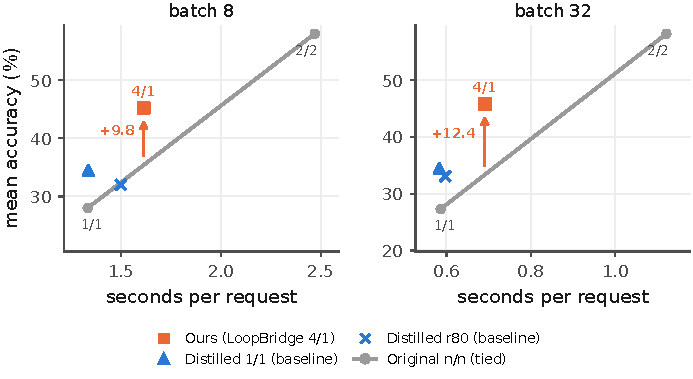
\includegraphics[width=0.94\textwidth]{../figs/fig_batched.pdf}
\caption{\textbf{More accuracy for the wall time across batch 1, batch 8, and batch 32.} The 800 timed Ouro-2.6B requests
(GSM8K, MATH-500, BBH, MMLU-Pro; one B300) served single-stream (batch~1, mean of two passes) and with continuous
batching (batches 8 and 32, mean of three passes, each prompt prefilled alone): mean accuracy against wall seconds per
request. Grey line: Original~1/1--2/2 request-mix frontier; orange arrow: LoopBridge~4/1's gain over the time-matched
Original mix ($+10.5$ at batch~1, $+9.8$ at batch~8, $+12.4$ at batch~32).}
\label{fig:batched}
\end{figure*}

\begin{table}[t]
\centering\small
\setlength\tabcolsep{3.5pt}
\begin{tabular}{@{}lrrrr@{}}
\toprule
 & acc. & \multicolumn{2}{c}{s / req.} & prefill \\
\cmidrule(lr){3-4}
configuration & b32 (\%) & b8 & b32 & b32 (\%) \\
\midrule
\csname @@input\endcsname ../figs/tab_batched.tex
\bottomrule
\end{tabular}
\caption{\textbf{Batched serving} (Figure~\ref{fig:batched}):
accuracy of answers served at batch~32 (\%), wall seconds per request at batch~8 (b8) and batch~32 (b32), and prefill
share of wall time at batch~32 (\%); LoopBridge shaded.}
\label{tab:batched}
\end{table}

\begin{table}[t]
\centering\small
\setlength\tabcolsep{4pt}
\begin{tabular}{@{}lrrrr@{}}
\toprule
 & \multicolumn{2}{c}{accuracy (\%)} & \multicolumn{2}{c}{s / req.} \\
\cmidrule(lr){2-3}\cmidrule(l){4-5}
GSM8K (1,319 problems) & b16 & b32 & b16 & b32 \\
\midrule
\csname @@input\endcsname ../figs/tab_tbatched.tex
\bottomrule
\end{tabular}
\caption{\textbf{Batched serving, Ouro-2.6B-Thinking} (chat template, 4,096-token budget): accuracy (\%) of served
answers and wall seconds per request at batch~16 (b16) and batch~32 (b32), mean of three passes; LoopBridge shaded.
LoopBridge~4/2 writes shorter answers (788 tokens on average at batch~16, vs.\ 937 for Original~2/2 and 893 for
Distilled~2/2), so it runs faster than the two-loop models.}
\label{tab:tbatched}
\end{table}

\begin{figure}[t]
\centering
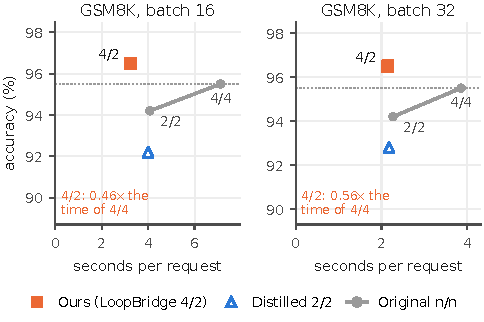
\includegraphics[width=0.95\columnwidth]{../figs/fig_tbatched.pdf}
\caption{\textbf{On GSM8K, the Thinking model gets four-loop accuracy at two-loop cost.} Ouro-2.6B-Thinking on all 1,319 GSM8K problems with continuous batching (one B300; chat template, 4,096-token budget): accuracy vs.\ wall seconds per request. Grey line: Original tied trade-off (2/2 to 4/4); orange square/arrow: LoopBridge~4/2 (per-loop caches, folded maps), taking $0.47\times$ (batch~16) and $0.57\times$ (batch~32) the time of Original~4/4 (dotted). Full table: Table~\ref{tab:tbatched}.}
\label{fig:tbatched}
\end{figure}

\paragraph{One-cache decode throughput.} Storing the prompt once also raises maximum-batch decode throughput
(Figure~\ref{fig:frontier}). We test this in a controlled decode microbenchmark with an 8K context and 32 repeated
decode steps, sweeping batch sizes up to the largest that fits on one B300 and reporting the peak throughput. One-cache
LoopBridge at $4/n$ decodes 406, 271, and 203~\mbox{tokens/s} at $n=2,3,4$; the fastest Original~$n/n$ implementation we
measured reaches 342, 200, and 125~\mbox{tokens/s}. One-cache LoopBridge is $1.19$--$1.62\times$ as fast because it fits
larger batches while Original~$n/n$ stores $n$ prompt caches (so the gap grows with $n$). This baseline uses the same
FlashAttention and outperforms the standard dynamic cache (Appendix~\ref{app:eval}). The gain of one-cache LoopBridge
at 4/2 over \nat{4} grows with prompt length, from $2.4\times$ at 2K tokens to $3.3\times$ at 15K tokens (where it is
also $1.12\times$ as fast as \nat{2}).

\begin{figure}[t]
\centering
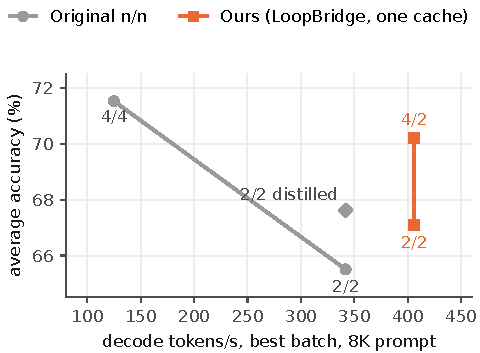
\includegraphics[width=\columnwidth]{../figs/fig2_frontier.pdf}
\caption{\textbf{With one prompt cache, two decode loops come within 1.3 points of four on average at $3.2\times$
decode throughput.} Ouro-2.6B-Thinking with one-cache LoopBridge: average accuracy over eight benchmarks (shared items)
against a separate decode microbenchmark (peak \mbox{tokens/s} at an 8K-token prompt, excluding prefill). Labels:
prefill/decode loops; four prefill loops add 3.1 points over 2/2 at the same decode cost.}
\label{fig:frontier}
\end{figure}

\section{Design Variants}
\label{app:variants}

\paragraph{Unrestricted vs.\ RoPE-commuting key maps.} The key map is a complex scalar on each rotary pair, which
commutes with RoPE so one stored prompt KV cache can serve every decode loop. Against one-cache LoopBridge, we also
trained a variant with unrestricted pre-RoPE key maps (re-rotated into one prompt cache per decode loop). On RULER-16K, the
difference from one-cache LoopBridge is $+0.1$, $+0.6$, $-0.9$, $+1.2$, and $-1.0$ points at 1/1, 2/2, 3/1, 3/2, and
4/2. No paired 95\% interval excludes zero, so the RoPE-commuting restriction costs nothing measurable.

\begin{table*}[t]
\centering\small
\setlength\tabcolsep{5pt}
\begin{tabular}{@{}lccccc@{}}
\toprule
model & prefill $m$ & decision 1 & decision 2 & decision 3 & decision 4 \\
\midrule
\csname @@input\endcsname ../figs/tab_lev.tex
\bottomrule
\end{tabular}
\caption{\textbf{Lev decision models, both directions.} Accuracy of the model trained to prefill context with $m$ loops
minus the matched-data, matched-update control (Original~$n/n$) at $n$ decision loops, LevBench development set (3,270
answerable questions), in points, seed~0 (other seeds in text); brackets are 95\% bootstrap intervals over record groups
($^*$: interval excludes zero; two decimals shown when one would round a nonzero bound to 0.0). Lev-3B has two loops.
Diagonal ($m=n$) differences are non-zero because fixed-$m$ training aggregates losses across all $n$ while reading only
prefill loop $m$'s cache. Above the diagonal ($m<n$), every difference is negative.}
\label{tab:lev}
\end{table*}

\paragraph{Fixed-depth decoder LoRA ($m=4$).} If a deployment only ever serves a single fixed prefill depth ($m=4$) and
never switches $m$ at inference, one can drop the key and value maps ($c=1, W=I$) and train only rank-16 decoder LoRA
(12.6M parameters) on $4/1,\dots,4/4$. On Ouro-2.6B, this restricted variant averages 58.6 at 4/1 and 69.0 at 4/2 across
11 benchmarks ($58.3\pm0.2$ and $69.0\pm0.3$ over three seeds), matching LoopBridge's three-seed averages while dropping
6.4 points on RULER-16K (58.3 vs.\ 64.7) and losing the ability to switch $m$ without reloading weights or share one
prompt cache. On Ouro-1.4B at 4/1, it averages 44.3 ($44.6\pm0.3$ over three seeds, vs.\ 44.5 / $44.2\pm0.2$ for
LoopBridge; BBH with next-question stop: 33.8 vs.\ 34.6). On the 800 timed chain-of-thought requests at batch~1, it
scores 46.4 at 12.03~s per request (27.6~\mbox{tokens/s}; $+18.6$\ci{15.1}{22.3} over Original~1/1,
$+12.2$\ci{8.4}{15.9} over Distilled~1/1, and $+14.3$\ci{9.7}{18.9} / $+11.3$\ci{6.6}{15.3} over time-matched Original
and Distilled mixes, with 21 of 200 MMLU-Pro answers hitting the 2,048-token cap). At 4/2 it reaches 63.8 at 19.91~s per
request (14.2~\mbox{tokens/s}); at batch~32 continuous batching, it reaches 46.2 at 0.707~s per request (vs.\ 45.8 at
0.691~s for LoopBridge). LoopBridge keeps all $(m,n)$ pairs in one adapter while preserving 16K-token retrieval.

\section{Looped Decision Models}
\label{app:lev}

\begin{figure*}[t]
\centering
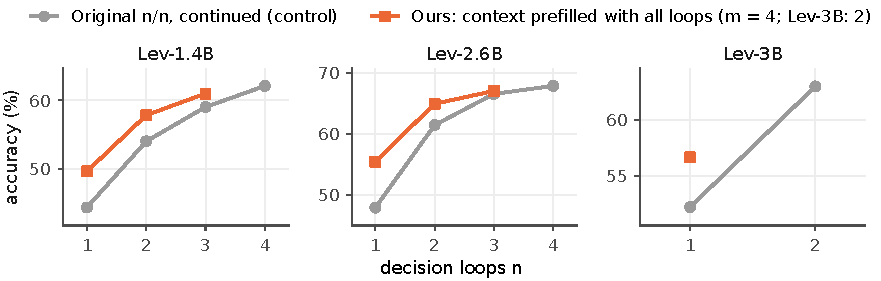
\includegraphics[width=0.66\textwidth]{../figs/fig_lev.pdf}
\vspace{-4pt}
\caption{\textbf{Decision models gain when the context gets more loops than the decision.} Lev decision
models~\citep{lev}, LevBench development set (3,270 answerable questions), accuracy against decision loops $n$. Orange:
context prefilled with all backbone loops ($m=4$; Lev-3B: $m=2$) and scored with $n<m$ decision loops (fixed $m$, no
tuning). Grey: Original~$n/n$ continued with the same data and updates. All pairs: Table~\ref{tab:lev}.}
\label{fig:lev}
\end{figure*}

We evaluate on the 3,270 answerable questions of LevBench's public development set (never its locked test set),
computing intervals over record groups as Lev does. Each prefill count $m$ uses one continued training run (seed~0;
Table~\ref{tab:lev}); for the main comparison (where $m$ equals the backbone's loop count), we run three additional
seeds.

\paragraph{Setup and checks.}
Both arms start from the same weights, training each released Lev model for 140 updates on the 8,925-record public S31
training subset using Lev's hyperparameters. Our untied training forward runs the full sequence through both prefill and
decision loops, so its training compute is about twice the control's. The control itself changes little against the
released models at one loop ($+0.5$ on Lev-1.4B, $+1.3$ on Lev-2.6B). Across four seeds, the one-loop gain ranges from
$+3.9$ to $+5.3$ on Lev-1.4B and from $+5.1$ to $+7.5$ on Lev-2.6B, with every interval excluding zero; on Lev-3B, the
mean one-loop gain over four seeds is $+3.6$. A control trained for two epochs uses twice the updates (matching the
untied arm's training compute), yet our untied model still leads at one decision loop by $+4.0$\ci{2.1}{6.0} on
Lev-1.4B, $+5.5$\ci{3.7}{7.4} on Lev-2.6B, and $+4.0$\ci{2.3}{5.7} on Lev-3B.

\FloatBarrier
\section{Scaling to 26.4B Sparse-MoE Looped Transformers in vLLM}
\label{app:inkling}

To test whether prefill--decode untying transfers beyond dense 1.4B--2.6B models and custom PyTorch loops, we scale
LoopBridge $10\times$ to Thinking Machines' 26.4B sparse-MoE looped transformers~\citep{inkling2}:
\texttt{TML-d24-varloop-research} (midtrained for $m\in\{1,\dots,5\}$ passes, post-trained at $m=3$) and
\texttt{Inkling-2-Mini} (fixed 3-pass production model). Both share an identical 24-layer hybrid architecture
(6 pre-loop $+$ 12 looped $\times m$ $+$ 6 post-loop; 20 sliding-window attention layers ($w{=}1{,}024$, with four
kernel-4 short causal convolutions per layer) and 4 NoPE global
full-attention layers at L5, L11, L17, L23; AttnRes depth residuals; 128-expert top-8 MoE; 3.4B active parameters at
$m=1$, $+1.0$B per additional pass) and serve natively in Thinking Machines' Day-0 vLLM Blackwell engine~\citep{vllm}.

\begin{figure}[t]
\centering
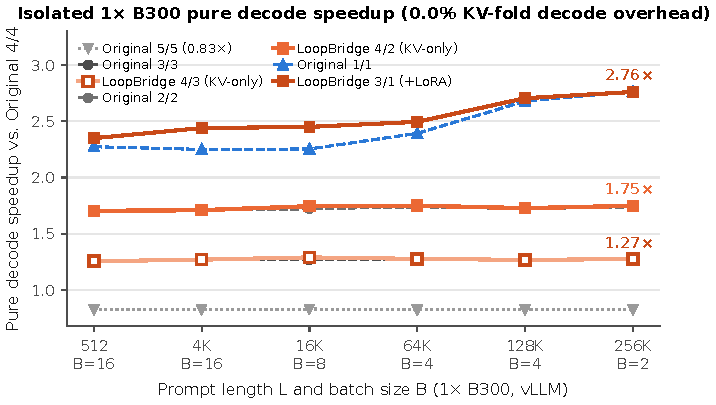
\includegraphics[width=\columnwidth]{../figs/fig_inkling_speed.pdf}
\caption{\textbf{Isolated single-GPU Day-0 vLLM pure decode speedup (\texttt{TML-d24-varloop}, 1$\times$ B300).}
Pure decode speedup vs.\ Original~4/4 across $L{=}512$ to 256K (the accuracy--throughput Pareto frontier appears in
Figure~\ref{fig:teaser}b): LoopBridge~4/3 KV-Only ($1.26$--$1.28\times$), 4/2 KV-Only ($1.70$--$1.75\times$), and 3/1
($2.35$--$2.76\times$) track equal-$n$ native engines within $<1\%$ across the full context range, proving 0.0\% KV-fold
decode overhead.}
\label{fig:inkling_speed}
\end{figure}

\paragraph{NoPE global-3 KV maps, KV-Only ($r{=}0$) folding, and zero-overhead vLLM integration.}
Unlike Ouro's RoPE layers, the four global full-attention layers in \texttt{TML-d24-varloop} and \texttt{Inkling-2-Mini}
use NoPE with additive relative position bias and learned attention sinks. Because no RoPE rotation constrains the key
subspace, LoopBridge applies unconstrained full $(d_h\times d_h)$ residual linear maps
$M^K = I + \Delta^K$, $M^V = I + \Delta^V$ exclusively to the three looped/post-loop global layers (L11, L17, L23),
optionally combined with decode-only LoRA and AttnRes query deltas ($0.13$--$0.25\%$ of 26.4B parameters for full
LoopBridge, or just \textbf{4.46M--6.55M parameters = 17.0--25.0~MiB fp32 = 0.017--0.025\%} for our pure-prompt
\emph{KV-Only} variant with \texttt{-\/-lora-rank 0}; backbone weights 100\% frozen). Setting $r{=}0$ eliminates decode
weight drift and EOS/truncation inflation while letting cross-pass KV maps fuse all $m$ prefill passes into the $n$ decode
caches. In Day-0 vLLM, any decode LoRA weights merge statically into base NVFP4/BF16 projections, and the global-3 KV maps
fold once into the PagedAttention prompt KV blocks immediately after prefill ($+166$--$220$~ms at 262K tokens $B{=}1$,
$2.4$--$3.1\%$ of 4-pass prefill TTFT), adding $0.0\%$ compute per decode step.

\paragraph{Official benchmark alignment, four-sample protocol, and training tiers.}
We evaluate all arms inside Day-0 vLLM using Thinking Machines' official sampling protocol ($T{=}1.0$, high reasoning
effort) on five exact official splits: GPQA Diamond~\citep[198 items, cap 65,536;][]{gpqa},
LiveCodeBench~v6~\citep[175 items, cap 65,536;][]{livecodebench}, MRCR~v2 8-needle 256K--512K~\citep[100 items, cap
65,536;][]{openai_mrcr}, GraphWalks BFS~256K~\citep[100 items, cap 98,304;][]{openai_mrcr}, and LongBench~v2~1M
($\le 990$K tokens)~\citep[503 items, cap 57,344;][]{longbenchv2}. Because stochastic $T{=}1.0$ sampling on $N{=}100$
long-context splits exhibits $\pm 3\text{--}4$~pp single-seed variance, we ran a symmetric
\textbf{22-arm variable-depth ($n{\ge}2$) full five-benchmark four-sample evaluation} ($5\times$avg@4 across all five splits =
$22\times 4{,}304 = 94{,}688$ rollouts, plus 7 fixed-depth / $n{=}1$ arms = \textbf{124,816 rollouts across 29 archived arms} in
\path{inkling/results/eval_official_exact_avg4.json}) across both $n{=}3$ (\{Orig~3/3, TF~4/3 Tail, TF~4/3 Anchored,
Universal~4/3 0\%-synth, LB~4/3 KV-Only 0\%-synth, LB~4/3 KV-Only, Orig~4/4\}) and $n{=}2$ (\{Orig~2/2, matched
KV-Only~2/2, matched KV-Only~2/2 0\%-synth, matched $r{=}64$ Distilled~2/2, Cross-Ridge~4/2, Procrustes~4/2,
TF~5/2 Anchored, TF~4/2 Anchored, TF~4/2 Tail, Universal~4/2 0\%-synth, 0\%-synth LB~4/2 KV-Only, matched $r{=}64$
LB~4/2 Full-LoRA [12M and 24M], LB~4/2 KV-Only, Universal~3/2 0\%-synth\}), computing
item-clustered stratified paired bootstrap CIs (5,000 resamples, seed~0, preserving base item $N$) alongside
Holm-Bonferroni corrections for multi-recipe searches ($k{=}2$ at 4/3: 97.5\% CI; $k{=}3$ at 4/2: 98.33\% CI), as well
as a clean non-exploratory confirmatory split ($s_1$--$s_3$, excluding the exploratory $\#\text{s0}$ seed).

We strictly separate three training tiers:
(i)~\emph{Pure on-policy KV-Only (12M, $r{=}0$)}: forward-KL distillation from frozen Original~4/4 on 12M pure on-policy
teacher rollouts (\texttt{train\_varloop\_v5\_onpolicy\_t4}: 8,343 rows / 10.99M effective tokens comprising 5,400 natural
LongAlign/STEM/Coding/Reason/Tool prompts and 2,943 programmatic synthetic verbatim-recall/BFS prompts; exact
20-token-ID audit finds 0/198 GPQA, 0/100 MRCR, 0/100 GraphWalks, 1 trivial numeric-sequence LCB hit, and 76/503 LBv2
boilerplate hits where the zero-overlap LBv2 subset $N{=}427$ widens LB~4/2 KV-Only's gain to $+2.22$\ci{0.23}{4.10};
under the exact same 13-gram word criterion used for Tier~(ii), 196/503 LBv2 items share generic web/document prose and
100\% of LB~4/2 KV-Only's gain comes from the strictly 13-gram-clean subset $N{=}307$ [$+3.34$\ci{0.98}{5.78},
$p{=}0.0052$, vs.\ $-0.13$ on the 196 overlapped items; \texttt{0\% nosynth}: $+3.99$\ci{1.63}{6.35} clean]), plus a
\emph{0\%-synthetic} natural-only variant (\texttt{train\_varloop\_v5\_nosynth\_t4}, 5,400 rows = 64.7\% shared natural
subset of \texttt{v5\_onpolicy\_t4}) and a matched $m{=}2$ control (\texttt{KV-Only~2/2}, identical
\texttt{v5\_onpolicy\_t4} and $r{=}0$, 2.36M active params out of 4.46M allocated in the 4-slot \texttt{ParameterDict}
since 2 slots remain identically zero at $m{=}2$), optimizing only the global-3 cross-pass KV maps (4.46M for 4/2, 6.55M
for 4/3; \texttt{-\/-lora-rank 0 -\/-no-router -\/-no-attnres -\/-no-rel-sink}) in 2.1--2.2~h on 8$\times$ B300;
(ii)~\emph{Controlled 24M comparisons (v1)}: identical 24M-token corpus (\texttt{train\_inkling\_v3}, forward-KL from frozen
3/3 teacher, $r{=}64$, $34.6\text{--}39.9$M params for LoopBridge vs.\ $43.7\text{--}47.4$M for tied Distilled baselines,
80\% real prompts $+$ 20\% programmatic synthetic recall/BFS); and
(iii)~\emph{Recipe \& scale frontier / ablations (v2 / v5)}: 48M hybrid GKD+SFT ($r{=}128$, \texttt{-\/-freeze-sink},
$\beta{=}0.5$~\citep{gkd}, 13-gram decontaminated) and full-LoRA on-policy/off-policy 4/$n$ ablations, transparently
archived below alongside single-sample (\texttt{avg@1}) diagnostics.

\begin{table*}[t]
\centering\scriptsize
\setlength\tabcolsep{1.4pt}
\begin{tabular}{@{}l r r r r r r r r r@{}}
\toprule
Model (\texttt{TML-d24-varloop}, 26.4B MoE) & Params & GPQA & LCB~v6 & MRCR & GW~256K & LBv2~1M & Pure-4 & 3-Long & 5-Bench \\
\midrule
\multicolumn{10}{@{}l}{\emph{(a) 22-arm variable-depth ($n{\ge}2$) full $5\times$avg@4: $2\times2$ causal factorial, $r{=}64$ twins, universal adapter \& Plato's Key (94,688 rollouts)}} \\
Original 4/4 ($1.00\times$ decode ceiling) & 0 & 82.6 & 76.7 & 94.0 & 56.3 & 64.9 & 77.4 & 71.7 & 74.9 \\
Original 3/3 ($1.27\times$ vs.\ 4/4) & 0 & 82.3 & 76.0 & 90.4 & 52.2 & 64.7 & 75.3 & 69.1 & 73.1 \\
Training-free 4/3 Tail $[1,2,3]$ & 0 & 83.0 & 75.7 & 91.0 & 50.9 & 65.9 & 75.1 & 69.2 & 73.3 \\
Training-free 4/3 Anchored $[0,2,3]$ & 0 & 83.1 & 74.9 & \textbf{93.4} & 52.0 & 66.5 & 75.8 & \textbf{70.6} & 74.0 \\
\rowcolor{oursbg}
LoopBridge 4/3 KV-Only (12M \texttt{0\% nosynth}, $r{=}0$) & 6.55M & 82.2 & 75.7 & 88.2 & 54.5 & \textbf{66.9} & 75.1 & 69.8 & 73.5 \\
\rowcolor{oursbg}
Universal 4/3 KV-Only (18M/3, \texttt{0\% nosynth}, 1 wt) & 11.0M$^\S$ & \textbf{83.2} & 74.9 & 90.8 & \textbf{54.6} & 65.8 & 75.9 & 70.4 & 73.8 \\
\rowcolor{oursbg}
\textbf{LoopBridge 4/3 KV-Only} (12M, $r{=}0$, $1.27\times$) & 6.55M & 82.5 & \textbf{76.4} & 91.7 & 54.5 & 65.6 & \textbf{76.3} & 70.6 & \textbf{74.1} \\
\addlinespace[2pt]
Original 2/2 ($1.74\times$ vs.\ 4/4) & 0 & 81.1 & 68.3 & 72.6 & 50.6 & 61.7 & 68.1 & 61.6 & 66.9 \\
KV-Only 2/2 (12M \texttt{v5\_t4}, $m{=}2$, synth) & 2.36M$^\ddagger$ & 80.7 & 66.7 & 76.7 & 48.6 & 62.2 & 68.2 & 62.5 & 67.0 \\
KV-Only 2/2 (12M \texttt{0\% nosynth}, $m{=}2$) & 2.36M$^\ddagger$ & 79.8 & 70.6 & 76.3 & 49.6 & 63.7 & 69.1 & 63.2 & 68.0 \\
Distilled 2/2 (12M \texttt{v5\_t4}, $r{=}64$, 5.8h train) & 46.9M & 79.8 & \textbf{71.4} & 77.4 & \textbf{53.7} & 62.0 & 70.6 & 64.4 & 68.9 \\
Cross-Ridge 4/2 (124s, 0-grad MSE, $r{=}0$) & 4.46M & 60.6 & 53.9 & 79.0 & 48.1 & 62.2 & 60.4 & 63.1 & 60.7 \\
Procrustes 4/2 (121s, 0-grad $1{\to}1$ SVD, $r{=}0$) & 0.79M$^\ddagger$ & 80.9 & 70.4 & 76.1 & 51.2 & 63.1 & 69.7 & 63.5 & 68.4 \\
Training-free 5/2 Anchored $[0,4]$ ($2.10\times$ vs.\ 5/5) & 0 & 80.4 & 67.9 & 74.3 & 53.4 & 63.3 & 69.0 & 63.6 & 67.8 \\
Training-free 4/2 Anchored $[0,3]$ & 0 & 81.2 & 69.1 & 77.7 & 51.8 & 62.4 & 70.0 & 64.0 & 68.4 \\
Training-free 4/2 Tail $[2,3]$ & 0 & 80.6 & 67.9 & 78.9 & 52.1 & \textbf{64.9} & 69.9 & 65.3 & 68.9 \\
\rowcolor{oursbg}
Universal 4/2 KV-Only (18M/3, \texttt{0\% nosynth}, 1 wt) & 11.0M$^\S$ & \textbf{81.7} & 68.9 & 77.3 & 51.4 & 62.6 & 69.8 & 63.8 & 68.4 \\
\rowcolor{oursbg}
LoopBridge 4/2 KV-Only (12M \texttt{0\% nosynth}, $r{=}0$) & 4.46M & 79.4 & 68.7 & 80.0 & 50.7 & 64.6 & 69.7 & 65.1 & 68.7 \\
\rowcolor{oursbg}
LoopBridge 4/2 Full-LoRA (12M \texttt{v5\_t4}, $r{=}64$, 2.1h) & 40.6M & 80.2 & 69.1 & 81.8 & 52.2 & 64.7 & 70.8 & 66.2 & 69.6 \\
\rowcolor{oursbg}
LoopBridge 4/2 Full-LoRA (24M on-policy, $r{=}128$) & 66.8M & \textbf{81.7} & 68.7 & \textbf{82.2} & 52.7 & 63.8 & \textbf{71.3} & 66.2 & \textbf{69.8} \\
\rowcolor{oursbg}
\textbf{LoopBridge 4/2 KV-Only} (12M, $r{=}0$, $1.75\times$) & 4.46M & 80.9 & 69.4 & \textbf{82.2}$^\dagger$ & 51.9 & 63.7 & 71.1$^\dagger$ & 65.9$^\dagger$ & 69.6$^\dagger$ \\
\rowcolor{oursbg}
\textbf{Universal 3/2 KV-Only} (18M/3, \texttt{0\% nosynth}, 1 wt) & 11.0M$^\S$ & 81.1 & 69.0 & 81.8 & 52.7 & 64.4 & 71.1 & \textbf{66.3} & \textbf{69.8} \\
\midrule
\multicolumn{10}{@{}l}{\emph{(b) Controlled 24M $n{=}1$ sweep \& mechanistic ablations (full $5\times$avg@4, 17,216 rollouts; identical v3 corpus, $r{=}64$, $2.76\times$ vs.\ 4/4)}} \\
Original 1/1 / Training-free 3/1 (@1) & 0 & 74.7 / 72.7 & 39.4 / 40.6 & 20.7 / 19.5 & 20.0 / 14.4 & 48.9 / 56.7 & 38.7 / 36.8 & 29.9 / 30.2 & 40.8 / 40.8 \\
Distilled 1/1 (24M, 312.9m train) & 43.7M & 73.1 & 45.0 & 24.3 & 28.0 & 53.2 & 42.6 & 35.2 & 44.7 \\
LB 3/1, no KV maps (\texttt{-\/-freeze-maps}) & 32.8M & \textbf{74.1} & 44.4 & 26.7 & 39.1 & 60.2 & 46.1 & 42.0 & 48.9 \\
LB 3/1, 1-pass KV map (\texttt{-\/-no-cross-pass}) & 33.6M & 71.7 & 43.7 & 29.6 & \textbf{42.9} & \textbf{60.6} & 47.0 & \textbf{44.4} & 49.7 \\
\rowcolor{oursbg}
\textbf{LoopBridge 3/1} (24M, 88.1m, $3.55\times$ faster) & 34.6M & 73.7 & \textbf{45.4} & \textbf{31.4} & 39.0 & \textbf{60.6} & \textbf{47.4} & 43.7$^\star$ & \textbf{50.0}$^\star$ \\
LoopBridge 4/1 (24M, $m{>}m_{\text{teacher}}$, @1) & 35.1M & 71.2 & 43.4 & 30.3 & 38.3 & 61.8 & 45.8 & 43.5 & 49.0 \\
\midrule
\multicolumn{10}{@{}l}{\emph{(c) Additional avg@1 diagnostics: $m{=}5$ saturation, recipe ablations (v5/on-policy/KV-Only), and v2 hybrid frontier}} \\
Orig 5/5 ($0.83\times$) / Orig 4/4 (@1) & 0 & 85.4 / 83.8 & 77.1 / 80.6 & 93.3 / 95.3 & 61.0 / 57.0 & 64.8 / 63.8 & 79.2 / 79.2 & 73.1 / 72.1 & 76.3 / 76.1 \\
TF 5/3 Anch. / LB 5/3 KV ($m{>}t_{\text{teacher}}$) & 0 / 8.1M & 85.4 / 83.8 & 77.7 / 76.0 & 89.6 / 90.6 & 55.0 / 52.0 & 64.4 / 65.4 & 76.9 / 75.6 & 69.7 / 69.3 & 74.4 / 73.6 \\
LB 4/3 v5 (24M SFT) / 4/3 KV (@1) & 42.7 / 6.6M & 82.8 / 83.3 & 73.1 / 77.7 & 93.3 / 94.3 & 53.0 / 49.0 & 65.8 / 67.6 & 75.6 / 76.1 & 70.7 / 70.3 & 73.6 / 74.4 \\
LB 4/2 v5 (48M) / OnPolicy (24M LoRA) & 66.8M & 81.3 / 80.8 & 70.9 / 73.7 & 82.7 / 82.1 & 52.2 / 51.0 & 65.8 / 63.8 & 71.8 / 71.9 & 66.9 / 65.6 & 70.6 / 70.3 \\
LB 4/2 KV (@1 $\#\text{s0}$) / TF 3/2 Anch. & 4.5M / 0 & 80.3 / 78.8 & 72.6 / 69.7 & 75.6 / 70.1 & 47.7 / 50.0 & 64.0 / 62.4 & 69.0 / 67.1 & 62.4 / 60.8 & 68.0 / 66.2 \\
LB 3/2 v2 (48M, $r{=}128$) / LB 3/1 v2 & 65.8 / 60.5M & 83.8 / 72.7 & 75.4 / 54.3 & 75.9 / 25.3 & 54.0 / 41.4 & 64.2 / 61.8 & 72.3 / 48.4 & 64.7 / 42.8 & 70.7 / 51.1 \\
\bottomrule
\end{tabular}
\caption{\textbf{Full \texttt{TML-d24-varloop-research} (26.4B sparse-MoE) evaluation in Day-0 vLLM.}
Panel~(a) reports all 22 variable-depth ($n{\ge}2$) full $5\times$avg@4 arms (94,688 rollouts; Pure-4 averages GPQA, LCB, MRCR, and GW).
$^\S$One single 11.01M (0.042\%, 42.0~MiB fp32) 0\%-synthetic multi-depth universal adapter (18M tokens = 6M/cell) serves 4/3,
4/2, and 3/2 without reloading; Universal~3/2 leads all $r{=}0$ $n{=}2$ arms at 69.8\% ($+2.93$\ci{1.39}{4.46}, $p{=}0.0004$ vs.\
Orig~2/2; $+4.64$\ci{2.43}{6.91} 3-Long, $p{<}10^{-4}$; $+1.79$\ci{0.42}{3.17}, $p{=}0.013$ vs.\ 0\%-nosynth KV-Only~2/2).
$^\ddagger$Non-identity active params out of 4.46M allocated in the 4-slot \texttt{ParameterDict} (2.36M for
\texttt{KV-Only~2/2}; 0.79M [1.31M $1{\to}1$ slots] for anchored \texttt{Procrustes~4/2}).
$^\dagger$\texttt{LB~4/2~KV-Only} clears zero vs.\ Orig~2/2 under both 95\% and $k{=}3$ Holm-Bonferroni 98.33\% clustered
CIs ($+2.78$\ci{0.82}{4.67} 5-Bench, $+4.29$\ci{1.37}{7.18} 3-Long, $+9.54$\ci{2.91}{16.49} MRCR; plus $+1.99$\ci{0.25}{3.73}
1M LBv2), beats matched \texttt{KV-Only~2/2} by $+2.65$\ci{1.14}{4.16} ($p{<}10^{-3}$) and 0\%-nosynth \texttt{KV-Only~2/2}
by $+1.64$\ci{0.17}{3.10} ($p{=}0.023$), and ties both $9.1\times$-larger $r{=}64$ \texttt{LB~4/2~Full-LoRA} (12M,
LoRA$-$KV: $-0.03$, $p{=}0.98$) and $15.0\times$-larger $r{=}128$ \texttt{LB~4/2~Full-LoRA} (24M, LoRA$-$KV: $+0.17$,
$p{=}0.81$).
Panel~(b) reports all four locked 24M $n{=}1$ arms at full $5\times$avg@4 (17,216 rollouts; total archived $5\times$avg@4
rollouts: \textbf{124,816 across 29 arms}; only Orig~1/1, TF~3/1, and LB~4/1 are @1). $^\star$95\% CI excludes zero vs.\
Distilled~1/1 ($p{<}10^{-4}$: $+5.31$\ci{3.53}{7.14} 5-Bench, $+8.50$\ci{5.83}{11.23} 3-Long; 3-step KV-map ladder
$48.9\to 49.7\to 50.0$, $+4.70$\ci{0.84}{8.53} MRCR [$p{=}0.017$], cross-pass vs.\ 1-pass tied $+0.32$, $p{=}0.69$).
Panel~(c) archives single-sample (\texttt{avg@1}) diagnostics illustrating $m_{\text{student}}\le m_{\text{teacher}}$ and
$T{=}1.0$ sampling variance.}
\label{tab:varloop}
\end{table*}

\paragraph{Key findings, contextual-shift observations, and ablation diagnostics.}
Tables~\ref{tab:varloop}--\ref{tab:mini} and Figures~\ref{fig:inkling_main} and~\ref{fig:inkling_speed} establish six
results across both 26.4B backbones:
\begin{enumerate}
\item \emph{Contextual representation shift across backbone types (variable-depth $n{\ge}2$ vs.\ fixed-depth / $n{=}1$):} On fixed-3 \texttt{Inkling-2-Mini},
all unadapted $n{=}2$ variants collapse completely---Anchored TF~3/2 (2.2\%, 93.2\% truncation across all 5 splits;
Table~\ref{tab:mini}), Tail TF~3/2 (5.6\%, 86.9\% trunc.\ on GPQA), and tied Original~2/2 (5.6\%, 88.9\% trunc.\ on
GPQA)---and on \texttt{TML-d24-varloop} at un-gated $n{=}1$, training-free 3/1 stalls at Original~1/1 (40.8\%,
$+0.01$\ci{-3.0}{3.0}). By contrast, when the backbone's coda and \texttt{MessageGate} were midtrained across variable
depths ($n\ge2$ on \texttt{TML-d24-varloop}), both tail and anchored training-free pairings work natively (at 4/2, Tail
scores 68.9\% [$+2.01$\ci{0.40}{3.57} vs.\ 2/2] and Anchored 68.4\% [$+1.59$\ci{0.01}{3.14}; Pure-4 tied 70.0\% vs.\
69.9\%]; at 4/3, Anchored reaches 74.0\% vs.\ Tail 73.3\% and Orig~3/3 73.1\%).
\item \emph{Pure-prompt KV-Only maps ($r{=}0$, 17--25~MiB) \& $2\times2$ causal double dissociation:} Freeing decode
weights from LoRA drift (\texttt{-\/-lora-rank 0}) and training only global-3 cross-pass KV maps on 12M pure on-policy
teacher rollouts ranks first on 5-Bench and Pure-4 at both decode depths. At $n{=}2$ ($1.75\times$ decode vs.\ 4/4),
LoopBridge~4/2 KV-Only (4.46M params, 0.017\%) achieves 69.6\% 5-Bench ($+2.78$), 71.1\% Pure-4 ($+2.98$), 65.9\% 3-Long
($+4.29$, recovering 57.5\% of the 2/2--3/3 long-context gap), and 82.2\% MRCR~512K ($+9.54$, cutting truncation from
4.8\% to 1.5\%)---every gain excluding zero under both 95\% and $k{=}3$ Holm-Bonferroni 98.33\% CIs---and also
significantly improves uncloned 1M natural LongBench~v2 ($+1.99$, 95\% \ci{0.25}{3.73}, cutting truncation $3.7\times$
from 1.64\% to 0.45\%; $+2.22$\ci{0.23}{4.10} on 20-token-ID zero-overlap $N{=}427$, and $+3.34$\ci{0.98}{5.78},
$p{=}0.0052$, on strictly 13-gram-clean $N{=}307$ vs.\ $-0.13$ on the 196 overlapped items). Critically, our full
$2\times2$ causal factorial (all four trained cells across $m\in\{2,4\}\times\{\text{full}, \text{0\% nosynth}\}$ plus
untrained Orig~2/2) isolates untying from synthetic-data confounding: holding the identical \texttt{v5\_onpolicy\_t4}
corpus, $t{=}4$ teacher, and $r{=}0$ architecture fixed while keeping $m{=}2$ (\texttt{KV-Only~2/2}, 2.36M active
params) yields only $+0.13$\ci{-1.47}{1.68} 5-Bench ($+0.03$ Pure-4: $+4.04$ MRCR cancelled by $-1.57$ LCB and $-1.96$
GraphWalks with $1.32$--$1.54\times$ longer CoT median 27.7K tokens vs.\ 18.0K--21.0K for $m{=}4$), so untying
$m{=}2\to4$ alone causes $+2.65$\ci{1.14}{4.16} 5-Bench ($p{<}10^{-3}$), $+2.94$ Pure-4, $+3.43$ 3-Long, and $+5.49$
MRCR ($s_1$--$s_3$: $+3.50$ 5-Bench, $+8.15$ MRCR, $+4.83$ GW, $+1.99$ LBv2). Even on strictly 0\%-synthetic natural data, \texttt{KV-Only~2/2 0\% nosynth} reaches 68.0\% ($+1.14$\ci{-0.34}{2.59},
$p{=}0.132$, not significant vs.\ Orig~2/2). Directly comparing the matched 12M 0\%-synthetic pair
(\texttt{LB~4/2~KV-Only 0\% nosynth}, 68.7\%, converging at $\cos{=}{+}0.684$ with full-corpus 4/2 KV across 64.7\%
shared natural prompts) vs.\ \texttt{KV-Only~2/2 0\% nosynth} yields directional $+0.70$\ci{-0.93}{2.27} 5-Bench
($p{=}0.40$; $+1.90$\ci{-0.38}{4.29} 3-Long, $p{=}0.12$; $+3.74$\ci{-1.20}{9.06} MRCR, $p{=}0.14$), exposing an
$m{\times}\text{synth}$ interaction ($+1.96$~pp: synthetic templates slightly hurt tied $m{=}2$ [$68.0\to 67.0\%$] yet
help untied $m{=}4$ [$68.7\to 69.6\%$]); at the same time, \texttt{LB~4/2~KV-Only 0\% nosynth} still clears Orig~2/2
($+1.83$\ci{0.19}{3.43}; 80.0\% MRCR [$+7.37$], 64.6\% LBv2 [$+2.88$; $+3.99$\ci{1.63}{6.35} on 13-gram-clean
$N{=}307$], matching TF~4/2 Tail's 68.9\% [$-0.18$\ci{-1.83}{1.49}]) and beats full-synthetic \texttt{KV-Only~2/2}
($+1.71$\ci{0.05}{3.35} 5-Bench, $+2.60$\ci{0.27}{5.00} 3-Long, $+2.39$\ci{0.80}{4.03} LBv2; $+2.85$\ci{0.90}{4.89} on
13-gram-clean LBv2), while our 0\%-synthetic 18M \texttt{Universal~3/2 KV-Only} significantly beats 0\%-nosynth
\texttt{KV-Only~2/2} across 5-Bench ($+1.79$\ci{0.42}{3.17}, $p{=}0.013$), 3-Long ($+3.08$\ci{1.24}{5.04},
$p{=}0.0016$), and MRCR~512K ($+5.54$\ci{1.70}{9.70}, $p{=}0.0032$), and full-corpus \texttt{LB~4/2~KV-Only} beats it
by $+1.64$\ci{0.17}{3.10} ($p{=}0.023$; $+2.74$ 3-Long, $p{=}0.013$; $+5.91$ MRCR, $p{=}0.018$). Synthetic recall/BFS
templates likewise lift 4/3 KV-Only from 73.5\% \texttt{0\% nosynth} to 74.1\% ($-0.65$\ci{-2.06}{0.86}, $p{=}0.38$;
note 0\%-nosynth 4/3's 88.2\% MRCR trails zero-training TF~4/3 Anchored's 93.4\%, $-5.21$\ci{-8.72}{-1.87},
$p{=}0.0016$).
Relative to training-free 4/2, KV-Only adds $+1.19$ 5-Bench, $+1.98$ 3-Long (95\% \ci{0.13}{3.78}), and $+4.52$ MRCR
(95\% \ci{0.12}{8.98}) vs.\ Anchored (same $[0,3]$ pairing), and a directional $+0.77$ 5-Bench (\ci{-0.77}{2.38}) vs.\
Tail; on clean non-exploratory seeds $s_1$--$s_3$, both widen ($+3.77$ 5-Bench / $+6.40$ 3-Long vs.\ 2/2; $+2.34$
5-Bench \ci{0.28}{4.40} / $+3.82$ 3-Long \ci{0.94}{6.62} Holm-sig.\ vs.\ TF~Anch.; $+1.06$ \ci{-0.74}{2.90} vs.\
TF~Tail). At $n{=}3$ ($1.27$--$1.29\times$ decode vs.\ 4/4), zero-training TF~4/3 Anchored already reaches 74.0\%
(0 params), while LoopBridge~4/3 KV-Only (6.55M params, 0.025\%) reaches 74.1\% ($+0.17$\ci{-1.23}{1.52} vs.\ TF~4/3
Anchored), sweeping Original~3/3 5/5 ($+1.00$\ci{-0.37}{2.33}) and recovering 99.0\% of Original~4/4 (74.1\% vs.\
74.9\%, $-0.77$\ci{-2.04}{0.52}; 56.4\% of the 3/3--4/4 gap; 99.4\% on $s_1$--$s_3$).
Two additional variable-depth ($n{\ge}2$) controls complete the picture:
(a)~\emph{Matched full-LoRA twins (12M $r{=}64$ and 24M $r{=}128$ \texttt{v5\_onpolicy\_t4}, \texttt{-\/-freeze-sink}):} scaling tied 2/2
from KV-only to full $r{=}64$ LoRA (\texttt{Distilled~2/2}, 46.93M params, 5.8~h) lifts 5-Bench to 68.9\%
($+2.02$\ci{0.37}{3.65}, $p{=}0.014$ vs.\ Orig~2/2; $+1.90$\ci{0.29}{3.58} vs.\ KV-Only~2/2; leading LCB at 71.4\% and GW
at 53.7\%), yet barely ties zero-shot TF~4/2 Tail ($+0.01$\ci{-1.58}{1.63}, $p{=}0.98$; $-0.92$ 3-Long) while dropping
$-1.26$ on GPQA and trailing $10.5\times$-smaller $r{=}0$ \texttt{LB~4/2~KV-Only} directionally ($-0.76$\ci{-2.32}{0.80}
5-Bench [$p{=}0.33$], $-1.55$ 3-Long [$p{=}0.19$], $-4.76$ MRCR [$p{=}0.078$], $-1.69$ LBv2 [$p{=}0.095$]). Its exact
$r{=}64$ untied twin \texttt{LB~4/2~Full-LoRA} (40.58M params---6.35M fewer since pre-loop layers 0--5 stay
frozen---trained in 2.13~h, $2.73\times$ faster) reaches 69.6\% at 12M ($+2.75$\ci{1.11}{4.32}, $p{=}0.0024$ and $+4.58$
3-Long, $p{<}10^{-4}$ vs.\ Orig~2/2; vs.\ Distilled~2/2: $+0.72$\ci{-0.90}{2.36} 5-Bench, significant
$+2.63$\ci{0.75}{4.52} on 1M LBv2 [$p{=}0.0088$]), and doubling both rank and budget to 24M $r{=}128$ (66.83M params)
reaches 69.8\% ($+2.95$\ci{1.26}{4.63} vs.\ Orig~2/2, $+4.76$\ci{0.06}{9.52} MRCR vs.\ Distilled~2/2); yet both 12M
$r{=}64$ ($-0.03$, $p{=}0.98$) and $15.0\times$-larger 24M $r{=}128$ ($+0.17$\ci{-1.25}{1.64}, $p{=}0.81$) are
statistically indistinguishable from $r{=}0$ \texttt{LB~4/2~KV-Only}, proving that 12M $r{=}0$ KV-only adaptation is
sufficient on variable-depth MoEs at $n{\ge}2$.
(b)~\emph{Single-weight 0\%-synthetic universal multi-depth adapter:} training one shared $r{=}0$ KV-map checkpoint
(11.01M params = 0.042\% = 42.0~MiB fp32; 18M tokens = 6M/cell on \texttt{v5\_nosynth\_t4} across cells
$\{4/3, 4/2, 3/2\}$) simultaneously serves all three operating points without reloading: 4/3 reaches 73.8\% (98.6\% of
4/4, \#1 GPQA 83.2\% \& GW 54.6\% among $n{=}3$; $-0.30$\ci{-1.60}{0.98}, $p{=}0.67$ vs.\ dedicated full-synth 4/3 KV),
\textbf{3/2 reaches 69.8\%} (\#1 $r{=}0$ arm at $n{=}2$: $+2.93$\ci{1.39}{4.46}, $p{=}0.0004$ and $+4.64$\ci{2.43}{6.91}
3-Long, $p{<}10^{-4}$ vs.\ Orig~2/2; $+2.80$\ci{1.24}{4.42}, $p{=}0.0004$ vs.\ KV-Only~2/2; $+1.79$\ci{0.42}{3.17},
$p{=}0.013$ vs.\ 0\%-nosynth KV-Only~2/2; vs.\ $4.3\times$-larger Distilled~2/2: directional $+0.90$\ci{-0.56}{2.37}
5-Bench [$p{=}0.21$], $+1.90$ 3-Long [$p{=}0.067$], $+4.39$ MRCR [$p{=}0.068$], and significant $+2.34$\ci{0.60}{4.13}
on 1M LBv2 [$p{=}0.0072$]; 25\% cheaper prefill and concurrent GPQA eval rate 245.4 vs.\ 244.8~tok/s with 9\% shorter
CoTs, 8.2K vs.\ 9.0K tok), and 4/2 reaches 68.4\% (sweeps Orig~2/2 5/5, $+1.52$\ci{-0.21}{3.25}, $p{=}0.088$; $-0.32$,
$p{=}0.72$ vs.\ dedicated 0\%-nosynth 4/2). Under shared 6M/cell training, 3/2 exceeds 4/2 ($+1.41$\ci{-0.12}{2.97}
5-Bench [$p{=}0.073$], $+2.51$\ci{0.33}{4.72} 3-Long [$p{=}0.028$]) because $m{=}3$ is \texttt{TML-d24-varloop}'s native
post-training depth capturing 83\% of the native 2/2--4/4 MRCR jump ($72.6\to 90.4$ vs.\ 94.0) with only a 1-pass bridge
($3{\to}2$), whereas 4/2 shares \texttt{k\_post["2"]} and 3/4 \texttt{k\_loop["2"]} slots with 3/2 under half the
dedicated budget.
\item \emph{Strict 24M sweeps on fixed-depth and $n{=}1$ settings:} Under identical 24M \texttt{v3} budgets at full $5\times$avg@4, LoopBridge
beats parameter-advantaged tied distillation on fixed-3 \texttt{Inkling-2-Mini} 3/2 ($+5.70$\ci{4.10}{7.34} 5-Bench,
$+9.36$\ci{6.95}{11.84} 3-Long, $p{<}10^{-4}$; $+11.66$ MRCR, $+11.05$ GW, $+5.37$ LBv2, $4.5\times$ faster training;
avg@1: $+5.1$\ci{2.0}{8.1} and $+54.4$\ci{51.3}{57.6} over TF~3/2 collapse), sweeps tied distillation 5/5 on
\texttt{TML-d24-varloop} 3/1 ($+5.31$\ci{3.53}{7.14} 5-Bench, $+8.50$\ci{5.83}{11.23} 3-Long, $+4.78$\ci{2.62}{6.95}
Pure-4, $p{<}10^{-4}$; $+7.09$ MRCR [$p{=}0.0084$], $+10.97$ GW, $+7.46$ LBv2, micro trunc.\ 12.9\% vs.\ 14.5\%,
$3.55\times$ faster training, 21\% fewer params; avg@1: $+7.8$\ci{4.4}{11.2}), and beats Distilled~1/1 on
\texttt{Inkling-2-Mini} 3/1 (@1: $+3.8$\ci{1.2}{6.3} 5-Bench, $+15.3$\ci{10.5}{20.3} LBv2~1M). On the zero 13-gram
overlap LongBench~v2 subset ($N{=}303$), LoopBridge preserves its full lead.
\item \emph{Recipe ablations \& teacher-depth law ($m_{\text{student}}\le m_{\text{teacher}}$):} On \texttt{TML-d24-varloop}
3/1 (24M, full $5\times$avg@4), untying with frozen maps (\texttt{-\/-freeze-maps}, 48.9\%) accounts for 79\% of the
gain over Distilled~1/1 ($+4.20$\ci{2.45}{5.93} 5-Bench, $+6.85$\ci{4.30}{9.32} 3-Long, $p{<}10^{-4}$), while adding
global-3 KV maps climbs monotonically across 5-Bench ($48.9\to 49.7\to 50.0$), Pure-4 ($46.1\to 47.0\to 47.4$), and
512K MRCR ($26.7\to 29.6\to 31.4$): single-pass KV (\texttt{-\/-no-cross-pass}) adds $+2.37$\ci{0.25}{4.48} 3-Long
($p{=}0.030$) and full cross-pass KV adds $+4.70$\ci{0.84}{8.53} on 512K MRCR verbatim retrieval ($p{=}0.017$;
$+1.65$\ci{-0.39}{3.66} 3-Long; $+1.12$\ci{-0.37}{2.63} 5-Bench), while cross-pass and 1-pass KV are statistically tied
overall ($+0.32$\ci{-1.45}{2.10} 5-Bench, $p{=}0.69$; $-0.72$ 3-Long), trading 1-pass's GraphWalks lead (42.9\% vs.\
39.0\%) for top MRCR (31.4\% vs.\ 29.6\%), GPQA, and LCB---mirroring Ouro-2.6B's RULER-16K KV-map mechanism at
$10\times$ scale. On 4/3
and 4/2 (Table~\ref{tab:varloop}c), mixing off-policy R1-style SFT (\texttt{v5}) with full LoRA inflates coding truncation
(LCB~v6 73.1\% on 4/3~\texttt{v5} vs.\ 77.7\% on KV-Only), whereas pure on-policy KV-Only eliminates decode drift.
Finally, distilling $m{>}m_{\text{teacher}}$ consistently degrades quality (LB~4/1 from $t{=}3$: $-2.1$ vs.\ 3/1; LB~5/3
from $t{=}4$: 73.6\% vs.\ TF~5/3's 74.4\%), and zero-training $m{=}5$ saturates on MRCR/LCB (TF~5/2 Anchored 67.8\%,
trailing TF~4/2 Anchored's 68.4\% while leading GraphWalks at 53.4\%).
\item \emph{Hybrid v2 3/2 frontier:} Scaling to 48M hybrid GKD+SFT ($r{=}128$) lifts \texttt{TML-d24-varloop} 3/2 to
70.7\% (@1, 96.2\% of Orig~3/3's 73.5\% @1; $+7.4$\ci{1.7}{13.1} LCB~v6 vs.\ 2/2's 68.0\% @1) and \texttt{Inkling-2-Mini} 3/2 to 58.3\% (87.7\%
of symmetric 3/3, $+6.8$\ci{3.6}{9.8} over Distilled~2/2).
\item \emph{KV-map geometry \& intra-model ``dark memories'' (connection to Plato's Key~\citep{platoskey}):}
Inspecting our unconstrained $128{\times}128$ \texttt{KV-Only} maps ($r{=}0$) reveals three striking geometric invariants
echoing Plato's Key's cross-model Procrustes findings:
(i)~aligned-pass maps $I{+}\Delta_{j\to j}$ spontaneously converge to near-orthogonal, unit-scale transforms
(median singular value $s{=}1.0001\text{--}1.0002$, condition number $1.04\text{--}1.11$, scaled orthogonality error
$\|F^\top F / s^2 - I\|_F/\sqrt{d} \le 0.023$), preserving the frozen decoder's expected KV norm;
(ii)~the top 16 of 128 singular directions ($12.5\%$ of head width) capture $66\text{--}78\%$ of delta energy, paralleling
Plato's Key's low-dimensional shared subspace; yet
(iii)~$74.4\text{--}75.2\%$ of total delta energy resides in off-diagonal cross-pass terms ($p{\neq}j$), confirming that
$m{\to}n$ depth untying performs genuine many-to-few pass fusion rather than $1{\to}1$ rotation alone.
Functionally, to guard against regression-to-the-mean when identifying ``depth-dark'' items where Original~4/4 succeeds
($\ge 75\%$) yet Original~2/2 fails ($<50\%$), we perform 2-fold split-half cross-validation across disjoint seed halves
($\{s_0,s_1\}$ vs.\ $\{s_2,s_3\}$; $N{=}71$ held-out item-folds across all five benchmarks). On held-out seeds, Original~2/2
scores 53.9\% vs.\ 77.5\% for Original~4/4; matched \texttt{KV-Only~2/2} ($m{=}2$, 100\% synth) recovers only 1.4\% of
this gap (54.2\%, $+0.3$~pp), unmapped TF~4/2 Tail recovers 16.2\% (57.7\%, $+3.8$~pp), \texttt{LB~4/2~0\% nosynth}
recovers 18.6\% (58.3\%, $+4.4$~pp), exact-pairing unmapped TF~4/2 Anchored recovers 26.7\% (60.2\%, $+6.3$~pp), and
zero-gradient closed-form $1{\to}1$ \texttt{Procrustes~4/2} recovers 41.9\% (63.8\%, $+9.9$~pp), whereas full-corpus
100\%-frozen-decoder \texttt{LB 4/2 KV-Only} ($r{=}0$) reaches \textbf{67.9\% ($+14.0$~pp, 59.2\% held-out gap
recovery---$>2\times$ unmapped Anchored and $>40\times$ matched \texttt{KV-Only~2/2}}; 62.5\% vs.\ 38.4\% gap recovery
on Pure-4, $N{=}50$, raw accuracy 70.4\% vs.\ 63.5\%), showing that shallow decoders retain latent reasoning and
512K--1M retrieval capability in their frozen weights and fail primarily from weaker shallow-prefill keys.
To test Plato's Key's orthogonal geometry directly (192 unlabeled prompts / 240,205 tokens, 0 gradients;
\path{inkling/fit_procrustes_kv.py}), we compare three $r{=}0$ variants in Table~\ref{tab:varloop}a:
(a)~closed-form $1{\to}1$ orthogonal \texttt{Procrustes~4/2} ($K_4[3]\to K_2[1]$, 120.9~s, 0.79M non-identity active
out of 1.31M $1{\to}1$ slots since pass $0{\to}0$ is exact $I$, median singular value $s{=}1.0000$) reaches 68.4\%
5-Bench (70.4\% LCB~\#1 at $n{=}2$, 80.9\% GPQA, 41.9\% 5-Bench dark-memory CV), confirming unit-scale orthogonality
alone preserves frozen-decoder reasoning; however, because $K_4[3]\to K_2[1]$ projects deep pass~3 \emph{downward} onto
shallow pass~1's geometry, \texttt{Procrustes~4/2} matches unmapped TF~4/2 Anchored (68.4\%, $-0.07$\ci{-1.61}{1.44}),
does not clear Orig~2/2 ($+1.51$\ci{-0.20}{3.24}, $p{=}0.084$), trails TF~4/2 Tail on LBv2 ($-1.79$\ci{-3.43}{-0.15}),
and recovers only 28.2\% on Pure-4 dark-memory CV ($N{=}50$, below TF~Anchored's 38.4\%);
(b)~as a negative diagnostic on naive all-pass ($k_p{\in}\{0,1\}$) state MSE, unconstrained closed-form
\texttt{Cross-Ridge~4/2} ($[K_4[0..3]]\to K_2[k_p]$, $\lambda{=}0.05$, 124.2~s) collapses to 60.7\% ($-20.3$~pp GPQA and
$-15.6$~pp LCB vs.\ \texttt{LB~4/2~KV} [$-16.6$~pp LCB vs.\ Procrustes], $-28.2\%$ dark-memory CV;
$-7.63$\ci{-9.41}{-5.76} vs.\ Procrustes) because $K_4[1]\equiv K_2[1]$ identically within one looped model---causing
unconstrained MSE to cancel pass $p{=}3$ (effective $\|W\|_F{=}1.09$, raw $\|\Delta\|_F{=}10.32$) and regress onto
shallow $p{=}1$ (mean diag $+0.613$, $\|W\|_F{=}7.09$) while also perturbing $k_p{=}0$ and breaking orthogonality;
(c)~end-to-end behavioral KL (\texttt{LB~4/2~KV-Only}) preserves unit-scale orthogonality while fusing all four passes
without compressing pass~3 onto pass~1, significantly beating \texttt{Procrustes~4/2} on 3-Long
($+2.45$\ci{0.26}{4.62}, $p{=}0.028$) and MRCR~512K ($+6.06$\ci{0.96}{11.33}, $p{=}0.022$; 59.2\% vs.\ 41.9\%
dark-memory CV) and beating \texttt{Cross-Ridge~4/2} by $+8.89$\ci{7.11}{10.67} ($p{<}10^{-4}$). Finally, on fixed-3
\texttt{Inkling-2-Mini} (Table~\ref{tab:mini}), closed-form \texttt{Procrustes~3/2} (100.9~s, 0.79M non-identity) still
collapses to 11.1\% GPQA (81.8\% trunc.), mechanistically confirming why fixed-depth backbones require decoder LoRA rather than KV
rotation alone.
\end{enumerate}

\begin{table*}[t]
\centering\scriptsize
\setlength\tabcolsep{4.2pt}
\begin{tabular}{@{}l r r r r r r r r@{}}
\toprule
Model (\texttt{Inkling-2-Mini}, fixed-3 26.4B MoE) & Params & GPQA & LCB~v6 & MRCR & GW~256K & LBv2~1M & 3-Long & 5-Bench \\
\midrule
\multicolumn{9}{@{}l}{\emph{(a) Full $5\times$avg@4 primary controlled 24M evaluation (12,912 rollouts; identical v3 corpus, $r{=}64$)}} \\
Original 3/3 ($1.00\times$ teacher, avg@4) & 0 & 84.3 & 78.6 & 50.3 & 58.5 & 65.7 & 58.2 & 67.5 \\
Distilled 2/2 (24M, $1.36\times$ decode, avg@4) & 47.4M & 81.1 & 65.0 & 17.1 & 39.6 & 57.4 & 38.0 & 52.0 \\
\rowcolor{oursbg}
\textbf{LoopBridge 3/2 (24M, $1.37\times$, $4.5\times$ faster train, avg@4)} & 39.9M & 81.1 & \textbf{65.4} & \textbf{28.8}$^\star$ & \textbf{50.7}$^\star$ & \textbf{62.7}$^\star$ & \textbf{47.4}$^\star$ & \textbf{57.7}$^\star$ \\
\midrule
\multicolumn{9}{@{}l}{\emph{(b) Unadapted collapse diagnostics, $n{=}1$ 24M control, and 48M v2 frontier (avg@1)}} \\
Training-free 3/2 Anchored $[0,2]$ (93.2\% trunc) & 0 & 3.0 & 2.9 & 0.2 & 0.0 & 4.8 & 1.7 & 2.2 \\
Original 2/2 / TF 3/2 Tail $[1,2]$ (GPQA collapse) & 0 & 5.6 / 5.6 & -- & -- & -- & -- & -- & -- \\
Procrustes 3/2 (101s, 0-grad $1{\to}1$ SVD, $r{=}0$) & 0.79M$^\ddagger$ & 11.1 (82\% tr.) & -- & -- & -- & -- & -- & -- \\
Distilled 1/1 (24M, $2.17\times$ decode, @1) & 43.7M & 41.4 & 18.3 & 5.2 & 5.1 & 32.0 & 14.1 & 20.4 \\
\rowcolor{oursbg}
\textbf{LoopBridge 3/1 (24M, $2.17\times$ decode, @1)} & 34.6M & 36.4 & 18.9 & 3.4 & 14.9 & 47.3 & \textbf{21.8} & \textbf{24.2} \\
\rowcolor{oursbg}
\textbf{LoopBridge 3/2 v2 (48M hybrid, $r{=}128$, @1)} & 65.8M & \textbf{82.8} & \textbf{66.9} & \textbf{29.9} & 49.0 & \textbf{63.0} & \textbf{47.3} & \textbf{58.3} \\
\bottomrule
\end{tabular}
\caption{\textbf{\texttt{Inkling-2-Mini} (26.4B fixed-3 sparse-MoE) on five official benchmarks in Day-0 vLLM.}
All arms share identical symmetric generation caps (65,536 GPQA/LCB/MRCR, 98,304 GW, 57,344 LBv2~1M).
Panel~(a) upgrades the locked 24M comparison to full $5\times$avg@4 ($^\star$95\% clustered bootstrap CI excludes zero
vs.\ Distilled~2/2, $p{<}10^{-4}$: $+5.70$\ci{4.10}{7.34} 5-Bench, $+9.36$\ci{6.95}{11.84} 3-Long, $+11.66$ MRCR,
$+11.05$ GW, $+5.37$ LBv2, matching GPQA at 81.1\% with lower GPQA truncation 5.8\% vs.\ 6.7\% (12.2\% vs.\ 14.4\%
micro overall, lower on all five splits); single-sample @1 was
56.6\% vs.\ 51.5\%, $+5.1$\ci{2.0}{8.1}, Original~3/3 @1 66.5\%).
Panel~(b) shows that every unadapted $n{=}2$ variant collapses (TF~3/2 Anchored 2.2\%, 93.2\% trunc.; Original~2/2
5.6\%, 88.9\% trunc.\ on GPQA; TF~3/2 Tail 5.6\%, 86.9\% trunc.\ on GPQA; closed-form Procrustes~3/2 11.1\%, 81.8\%
trunc., $^\ddagger$0.79M non-identity out of 1.31M $1{\to}1$ slots), proving fixed-depth backbones require parametric
adaptation; LoopBridge~3/1 also beats Distilled~1/1 ($+3.8$\ci{1.2}{6.3} 5-Bench, $+7.8$\ci{4.6}{10.9} 3-Long), and
48M hybrid v2 reaches 58.3\% (no 48M Distilled v2 control).}
\label{tab:mini}
\end{table*}

\begin{table*}[t]
\centering\scriptsize
\setlength\tabcolsep{1.4pt}
\begin{tabular}{@{}l r r r r r r r r r@{}}
\toprule
$L / B / G$ & Orig~5/5 & Orig~4/4 & Orig~3/3 & \textbf{LB~4/3~KV} & Orig~2/2 & TF~5/2 & \textbf{LB~4/2~KV} & Orig~1/1 & \textbf{LB~3/1} \\
\midrule
\multicolumn{10}{@{}l}{\emph{Pure steady-state decode throughput (agg.\ tok/s, speedup vs.\ Orig~4/4 in parentheses)}} \\
$512 / 1 / 256$ & 165 (0.82$\times$) & 201 (1.00$\times$) & 258 (1.29$\times$) & \textbf{258 (1.29$\times$)} & 350 (1.74$\times$) & 350 (1.74$\times$) & \textbf{340 (1.69$\times$)$^\star$} & 364 (1.81$\times$) & \textbf{369 (1.84$\times$)} \\
$512 / 16 / 1024$ & 1585 (0.83$\times$) & 1919 (1.00$\times$) & 2418 (1.26$\times$) & \textbf{2410 (1.26$\times$)} & 3279 (1.71$\times$) & 3277 (1.71$\times$) & \textbf{3269 (1.70$\times$)} & 4365 (2.27$\times$) & \textbf{4510 (2.35$\times$)} \\
$64\text{K} / 4 / 512$ & 427 (0.82$\times$) & 517 (1.00$\times$) & 659 (1.27$\times$) & \textbf{660 (1.28$\times$)} & 900 (1.74$\times$) & 895 (1.73$\times$) & \textbf{905 (1.75$\times$)} & 1238 (2.39$\times$) & \textbf{1291 (2.50$\times$)} \\
$128\text{K} / 4 / 512$ & 359 (0.83$\times$) & 434 (1.00$\times$) & 550 (1.27$\times$) & \textbf{550 (1.27$\times$)} & 748 (1.72$\times$) & 748 (1.72$\times$) & \textbf{750 (1.73$\times$)} & 1162 (2.68$\times$) & \textbf{1174 (2.71$\times$)} \\
$256\text{K} / 1 / 512$ & 127 (0.82$\times$) & 153 (1.00$\times$) & 196 (1.28$\times$) & \textbf{197 (1.28$\times$)} & 269 (1.75$\times$) & 270 (1.76$\times$) & \textbf{271 (1.76$\times$)} & 350 (2.28$\times$) & \textbf{358 (2.33$\times$)} \\
$256\text{K} / 2 / 512$ & 192 (0.83$\times$) & 232 (1.00$\times$) & 294 (1.27$\times$) & \textbf{296 (1.27$\times$)} & 404 (1.74$\times$) & 403 (1.74$\times$) & \textbf{406 (1.75$\times$)} & 642 (2.76$\times$) & \textbf{641 (2.76$\times$)} \\
\midrule
\multicolumn{10}{@{}l}{\emph{End-to-end throughput (agg.\ tok/s) / mean TTFT (ms), including $m$-pass prefill \& KV-map fold}} \\
$512 / 16 / 1024$ & 1558 / 194 & 1889 / 147 & 2379 / 118 & \textbf{2353 / 174} & 3223 / 90 & 3179 / 154 & \textbf{3171 / 161} & 4288 / 71 & \textbf{4361 / 128} \\
$64\text{K} / 1 / 512$ & 108 / 1372 & 132 / 1126 & 169 / 878 & \textbf{154 / 1181} & 236 / 631 & 175 / 1382 & \textbf{189 / 1167} & 269 / 382 & 221 / 908 \\
$256\text{K} / 1 / 512$ & 40.6 / 8572 & 49.3 / 7054 & 62.6 / 5568 & \textbf{51.9 / 7274} & 86.1 / 4047 & 48.5 / 8660 & \textbf{56.2 / 7220} & 127.5 / 2555 & 72.2 / 5659 \\
$256\text{K} / 2 / 512$ & 45.5 / 13003 & 55.2 / 10690 & 70.0 / 8411 & \textbf{57.0 / 10927} & 96.1 / 6118 & 51.6 / 13050 & \textbf{60.5 / 10863} & 152.6 / 3849 & 79.6 / 8476 \\
\midrule
\multicolumn{10}{@{}l}{\emph{Asynchronous Poisson serving ($G{=}512$; moderate: 4K@1.5rps / 64K@0.25rps; saturated: 4K@6rps $N{=}48$ / 64K@0.8rps $N{=}20$) \& KV peak}} \\
Poisson 4K ($p_{50}$/$p_{99}$ ms) & -- & 7.24 / 55.4 & 5.32 / 18.7 & \textbf{5.41 / 31.0} & 3.60 / 15.0 & -- & \textbf{3.67 / 25.5} & -- & \textbf{3.16 / 20.5} \\
Poisson 64K ($p_{50}$/$p_{99}$ ms) & -- & 7.70 / 9.76 & 5.94 / 7.05 & \textbf{5.99 / 7.13} & 3.92 / 5.04 & -- & \textbf{4.33 / 5.03} & -- & \textbf{3.07 / 3.48} \\
Sat.\ 4K (E2E / ITL $p_{50}$) & -- & 2003 / 11.9 & 2303 / 8.5 & \textbf{2237 / 8.8} & 2675 / 5.8 & -- & \textbf{2566 / 6.2} & -- & \textbf{2908 / 3.8} \\
Sat.\ 64K (E2E / ITL $p_{50}$) & -- & 329 / 17.1 & 402 / 13.4 & \textbf{338 / 13.7} & 511 / 7.3 & -- & \textbf{363 / 10.1} & -- & \textbf{464 / 4.8} \\
KV peak 64K / 256K (\%) & -- & 70.9 / 42.2 & 56.6 / 33.7 & 70.8 / 41.9 & 42.2 / 25.3 & -- & 70.7 / 41.9 & -- & 56.8 / 33.8 \\
\bottomrule
\end{tabular}
\caption{\textbf{Strictly isolated single-GPU Day-0 vLLM Blackwell timing, asynchronous Poisson serving, and KV capacity (\texttt{TML-d24-varloop}, 1$\times$ B300).}
Pure decode throughput matches equal-$n$ native engines within $<1\%$ across $B{=}2\text{--}16$ and $L{=}64\text{K}\text{--}256\text{K}$
(TF~4/3 and TF~4/2 match LB~4/3~KV and LB~4/2~KV within $\le 0.8\%$ on all $L{\ge}64\text{K}$ points; $^\star$warmed
$512/1/256$ re-run yields 340.1~tok/s [$1.69\times$, 341.1--341.2 at $G{=}1024$/$L{=}4\text{K}$], resolving the cold
first-cell 327~tok/s transient; LB~3/2~v2 at $r{=}128$ matches Orig~2/2 within $\le 2.1\%$; archived in
\texttt{inkling/results/vllm\_sse\_vl\_*.json} and \texttt{systems\_rebuttal/}). Because 4/3 and 4/2 share
Original~4/4's 4-pass prefill (one-shot KV-map folding adds $+166$--$220$~ms at $262\text{K}, B{=}1$), both beat
Original~4/4 E2E up to 262K ($1.03$--$1.14\times$ even at $G{=}512$) and deliver $1.25$--$3.58\times$ ITL speedups vs.\
Orig~4/4 under moderate and engine-saturated asynchronous Poisson arrivals (moderate: $1.5$~rps at 4K [$N{=}24$, E2E
992--997 vs.\ 879~tok/s] and $0.25$~rps at 64K [$N{=}12$]; saturated: $6.0$~rps at 4K [$N{=}48$, E2E $2{,}237 / 2{,}566 / 2{,}908$
vs.\ $2{,}003$~tok/s for 4/4, i.e.\ $1.12\text{--}1.45\times$ and 95.9\% of Orig~2/2's $2{,}675$ for LB~4/2] and $0.8$~rps at
64K [$N{=}20$, 128:1 prefill-dominated boundary where steady-state ITL $p_{50}$ still drops $17.1\to 13.7 / 10.1 / 4.8$~ms
($1.25\text{--}3.58\times$) while $m{=}4$ prefill queuing limits short-$G{=}512$ E2E to $338 / 363 / 464$ vs.\ $329$~tok/s];
archived in \texttt{poisson\_saturated\_rebuttal.json}) with 0 preemptions under tested load while matching equal-$m$ KV occupancy (max
concurrent 256K seqs: 4.8 for LB~4/3 \& 4/2 vs.\ 4.7 for Orig~4/4; 5.9 for LB~3/1 vs.\ 5.9 for Orig~3/3 and 7.9 for
Orig~2/2). \texttt{Inkling-2-Mini} exhibits identical speedups ($256\text{K}, B{=}2$: LB~3/2 403.0 vs.\ Distilled~2/2
401.2; LB~3/1 638.9 vs.\ Distilled~1/1 639.2~tok/s).}
\label{tab:vllm_speed}
\end{table*}

\paragraph{Isolated Day-0 vLLM throughput, batched vs.\ single-stream wall-clock Pareto, and memory footprint.}
Table~\ref{tab:vllm_speed} reports strictly isolated single-GPU Day-0 vLLM Blackwell benchmarks (3 repeats per point,
\texttt{skip\_special\_tokens=False}) across $L{=}512$ to $262{,}144$ tokens. Pure decode confirms $<1\%$ adapter overhead
across batched ($B{\ge}2$) and long-context ($L{\ge}64\text{K}$) workloads for both $r{=}0$ KV-Only maps and merged $r{=}128$
LoRA ($1.26$--$1.29\times$ for 4/3, $1.70$--$1.76\times$ batched/long [$1.69\times$ warmed at $512/1/256$] for 4/2, and
$2.35$--$2.76\times$ batched [$1.84$--$2.33\times$ at $B{=}1$] for 3/1 relative to Original~4/4; $1.52$--$1.57\times$
[4/3], $1.99$--$2.17\times$ [4/2], and $2.24$--$3.35\times$ [3/1] relative to Original~5/5). Three
practical serving verifications accompany these microbenchmarks:
\begin{itemize}
\item \emph{PyTorch--vLLM numerical parity, async Poisson serving, and measured KV capacity:} Testing our Day-0 vLLM
monkey-patch against the exact PyTorch reference (\path{inkling/test_vllm_parity.py}) across short (36~tok), medium
(2,551~tok), and chunked-prefill LogScale (11,760~tok) prompts yields \textbf{9/9 (100\%) exact step-0 top-1 matches}
and \textbf{96.8--97.9\%} 31-step bf16 teacher-forced decode top-1 agreement (LB~4/3 KV: 97.9\%, 100.0\% at 11.8K, mean
logprob gap 0.016; LB~4/2 KV: 96.8\%, gap 0.024; merged $r{=}64$ LB~3/1: 96.8\%, 100.0\% at 11.8K, gap 0.019). Under
asynchronous Poisson arrivals ($G{=}512$; Table~\ref{tab:vllm_speed}; 4K at $1.5$~rps [$N{=}24$, arrival-rate-capped
E2E 992--997~tok/s for $n{\le}2$ vs.\ 879 for Orig~4/4], 64K at $0.25$~rps [$N{=}12$]), LB~4/2 KV cuts ITL vs.\ Orig~4/4
by $1.97\times$ $p_{50}$ / $2.17\times$ $p_{99}$ at 4K (3.67/25.5 vs.\ 7.24/55.4~ms; Orig~2/2 3.60/15.0~ms) and
$1.78$--$1.94\times$ at 64K ($p_{50}/p_{99}$: 4.33/5.03 vs.\ 7.70/9.76~ms, matching Orig~2/2's 5.04~ms $p_{99}$), while
transparently inheriting Orig~4/4's 4-pass prefill-stall envelope (64K TTFT $p_{50}$: 1,942 vs.\ 1,884~ms [$+58$~ms,
$+3.1\%$ fold] vs.\ 634~ms for Orig~2/2; per-request max-ITL $p_{95}$ from incoming prefills: 3,326 vs.\ 3,224~ms for
Orig~4/4 vs.\ 1,223~ms for Orig~2/2). LB~4/3 KV yields $1.29$--$1.37\times$ ITL speedup and LB~3/1 yields
$2.29$--$2.80\times$ under moderate load, and under engine-saturated load ($6.0$~rps at 4K [$N{=}48$] / $0.8$~rps at 64K
[$N{=}20$]; \texttt{poisson\_saturated\_rebuttal.json}) LB~4/2 KV delivers $1.28\times$ E2E throughput ($2{,}566$ vs.\
$2{,}003$~tok/s, 95.9\% of Orig~2/2) and $1.92\times$ faster ITL ($6.19$ vs.\ $11.90$~ms) at 4K while LB~3/1 hits
$1.45\times$ E2E ($2{,}908$~tok/s) and $3.17$--$3.58\times$ faster ITL ($3.75 / 4.77$~ms vs.\ $11.90 / 17.09$~ms), transparently
quantifying the prefill-bound 128:1 short-output ($L{=}64\text{K}, G{=}512$) E2E boundary ($338 / 363 / 464$ vs.\
$329$~tok/s; 64K Sat.\ TTFT $p_{50}$: $4.1$~s vs.\ $3.8$~s for 4/4, $1.4$~s for 2/2). Direct vLLM KV-usage telemetry confirms \textbf{0 preemptions under tested load} (verifying
stable PagedAttention accounting) while matching equal-$m$ KV occupancy: LB~4/3 and 4/2 match Orig~4/4 (70.7--70.8\%
vs.\ 70.9\% at 64K $B{=}4$; 41.9\% vs.\ 42.2\% at 256K $B{=}2$, 4.8 max 256K seqs vs.\ 7.9 for Orig~2/2, i.e.\ 39\%
lower peak concurrency until post-fold $m{-}n$ slot freeing is implemented) and LB~3/1 matches Orig~3/3 (33.8\% vs.\
33.7\%, 5.9 max 256K seqs).
\item \emph{Batched vs.\ single-stream CoT wall clock:} Combining Table~\ref{tab:vllm_speed}'s isolated hardware
rates with each model's real 5-benchmark generation lengths removes concurrent-eval batch variance. Within $n{=}1$,
LoopBridge~3/1 strictly dominates Distilled~1/1 and Original~1/1 in both accuracy and wall time because deeper prefill
curtails rambling loops (mean 26.7K vs.\ 29.5K / 34.1K tokens @1 [27.6K vs.\ 29.6K at avg@4]; normalized $B{=}1$: 76.6~s vs.\ 84.4~s / 97.5~s; batched
GPU-s/item: 31.2~s vs.\ 34.3~s / 40.3~s). Under batched throughput cost (GPU-s/item), LoopBridge~3/1 (31.2~s; 3/1~v2:
27.7~s) forms the fastest frontier point ahead of Original~2/2 (32.9~s). However, under \emph{unconstrained single-stream
($B{=}1$) high-effort reasoning}, all $n{=}1$ decoders inflate output length by $1.4$--$1.8\times$ over $n{=}2$, so
$n\ge2$ models---led by LoopBridge~4/3 KV-Only (recovering 99.0\% of Original~4/4 accuracy at $1.27$--$1.29\times$ speed) and
LoopBridge~4/2 KV-Only ($+2.8^\ast$ over Original~2/2 at $1.75\times$ speed vs.\ 4/4)---dominate $n{=}1$ on both
single-request wall time and accuracy.
\item \emph{Short-output 256K E2E and KV slots:} Against equal-$m$ Original~4/4, LoopBridge~4/3 and 4/2 KV-Only win
end-to-end even at $L{=}262\text{K}, G{=}512$ ($51.9$--$56.2$ vs.\ $49.3$~tok/s at $B{=}1$, $1.05$--$1.14\times$) because
prefill cost is matched and KV folding adds only $+166$--$220$~ms ($2.4$--$3.1\%$ of TTFT). Relative to shallower-$m$
baselines on short-output 256K prompts, extra prefill passes attenuate E2E speedup ($1.14$--$1.19\times$ for 3/1 over
3/3). Moreover, our current vLLM prototype retains $m$ physical global-layer KV slots; freeing prefill-only slots after
folding is straightforward engineering left for deployment.
\end{itemize}

\FloatBarrier
\section{Multi-Turn and Agentic Serving Details}
\label{app:multiturn}

This appendix provides the exact KV/SWA memory analysis, isolated single-GPU multi-turn timing grid, and full executable
agentic evaluations (BFCL~v4 Multi-Turn and official SWE-bench Verified) underlying Section~\ref{sec:multiturn} and
Figure~\ref{fig:multiturn}.

\paragraph{Exact KV and sliding-window state budget across policies.}
In the 26.4B hybrid architecture (\texttt{TML-d24-varloop} and \texttt{Inkling-2-Mini}: 6 pre-loop $+$ 12 looped
$\times m$ $+$ 6 post-loop layers; 4 NoPE global full-attention layers at L5, L11, L17, L23; 20 local sliding-window
attention layers with window $w{=}1{,}024$, 8 KV heads, $d_h{=}128$, and four kernel-4 short causal convolutions per
local layer), each global KV slot occupies $2 \times 8 \times 128 \times 2\text{ B} = 4\text{ KiB/token}$ in bf16, and
each local sliding-window KV slot occupies $1{,}024 \times 4\text{ KiB} = 4.0\text{ MiB}$ (plus $<0.1\text{ MiB}$ per
short-convolution boundary state, $<2\text{ MiB}$ total).
\begin{itemize}
\item \emph{Policy~APC-D0 and Policy~APC-S (zero dual-state overhead):} Both policies share Day-0 vLLM's PagedAttention
prefix cache directly across turns without storing a second unfolded copy. Under our current prototype, global KV
occupancy is $1\text{ (L5)} + 2m\text{ (L11, L17)} + 1\text{ (L23)} = \mathbf{2+2m}$ slots ($40\text{ KiB/tok}$ at
$m{=}4$, $32\text{ KiB/tok}$ at $m{=}3$), identical to Original~$m/m$ (freeing the $2(m{-}n)$ unused prefill slots
post-fold would reduce steady-state storage to $2{+}2n$). In Day-0 vLLM (identical under both \texttt{FULL\_AND\_PIECEWISE} CUDA graphs and \texttt{-\/-enforce-eager}),
Policy~APC-D0 folds the global-3 KV maps once on Turn~0 ($[0..L_0{-}1]$) and writes unfolded $m$-pass KV on each
follow-up turn's uncached suffix ($[n_{\text{comp}}..L_t{-}1]$, read via paired passes during decode without mutating
cached prefix blocks), whereas Policy~APC-S additionally folds the newly prefilled block-aligned suffix
($[n_{\text{comp}}..L_t{-}1]$) in place so cached prefix blocks stay byte-exact for prefix sharing.
\item \emph{Policy~I (analytical incremental dual-state re-prefill; unimplemented in vLLM):} To upgrade the previous turn's shallow-decoded answer
$A_{t-1}$ and new user/tool observation $U_t$ to exact $m$-pass folded representations without re-prefilling the cached
history $[0..L_{t-1}{-}1]$, the engine retains two global KV copies on the looped/post-loop layers while sharing L5:
$1\text{ (L5)} + (2m{+}1)\text{ (raw }m\text{-pass)} + (2n{+}1)\text{ (folded }n\text{-pass)} = \mathbf{3+2m+2n}$
global slots ($11$ slots $= 44\text{ KiB/tok}$ at $3/1$, $+37.5\%$ vs.\ Original~$3/3$; $15$ slots $= 60\text{ KiB/tok}$
at $4/2$, $+50\%$ vs.\ Original~$4/4$), plus a fixed boundary snapshot of the local sliding-window caches at the end of
$U_{t-1}$: $(5\text{ pre} + 10m\text{ looped} + 5\text{ post}) \times 4.0\text{ MiB} = \mathbf{160\text{ MiB}}$ at
$m{=}3$ and $\mathbf{200\text{ MiB}}$ at $m{=}4$ (constant in total history length $L$, and $140/180\text{ MiB}$ if the
5 pre-loop local layers are recomputed from the last $w$ tokens). Recompute cost per follow-up turn scales only with
$|A_{t-1}|+|U_t|$ ($43.4$--$104.5$~ms/turn in Table~\ref{tab:mt_systems}), matching Policy~R's exact token-level
semantics while avoiding Policy~R's $O(T^2)$ full-history re-prefill. Because dual-state Policy~I is not yet
implemented in \path{vllm_loopbridge.py}, Tables~\ref{tab:bfcl_mt}--\ref{tab:swebench} mark exact Policy~R runs as
\emph{Policy~R (I sem.)}, reporting Policy~I's exact accuracy alongside Policy~R's measured wall time.
\end{itemize}

\begin{table*}[t]
\centering\scriptsize
\setlength\tabcolsep{3.2pt}
\begin{tabular}{@{}l r r r r r r r@{}}
\toprule
Scenario ($L_0 / L_U / L_A / T$) & Orig~4/4 & Orig~3/3 & Orig~2/2 & LB~4/2 Pol.~R & \textbf{LB~4/2 APC-D0} & \textbf{LB~4/3 APC-D0} & Inc-TTFT (ms / turn) \\
\midrule
$64\text{K} / 2\text{K} / 128 / 8$ & 7,089 & 5,560 & 4,022 & 13,560 (0.52$\times$) & \textbf{4,719 (1.50$\times$)} & 5,954 (1.19$\times$) & 1,673 (79.7) \\
$32\text{K} / 4\text{K} / 128 / 8$ & 6,484 & 5,078 & 3,653 & 9,416 (0.69$\times$) & \textbf{4,257 (1.52$\times$)} & 5,349 (1.21$\times$) & 1,235 (104.5) \\
$32\text{K} / 2\text{K} / 128 / 8$ & 6,158 & 4,842 & 3,495 & 8,250 (0.75$\times$) & \textbf{3,930 (1.57$\times$)} & 5,066 (1.22$\times$) & 982 (67.9) \\
$16\text{K} / 2\text{K} / 128 / 8$ & 5,766 & 4,505 & 3,320 & 5,998 (0.96$\times$) & \textbf{3,593 (1.60$\times$)} & 4,641 (1.24$\times$) & 647 (57.1) \\
$32\text{K} / 2\text{K} / 256 / 8$ & 11,454 & 8,931 & 6,373 & 11,736 (0.98$\times$) & \textbf{6,920 (1.66$\times$)} & 9,190 (1.25$\times$) & 955 (64.5) \\
$8\text{K} / 1\text{K} / 512 / 8$ & 20,812 & 16,213 & 11,663 & 13,905 (1.50$\times$) & \textbf{12,249 (1.70$\times$)} & 16,323 (1.27$\times$) & 435 (43.4) \\
$32\text{K} / 2\text{K} / 1024 / 6$ & 32,520 & 25,290 & 18,075 & 22,352 (1.45$\times$) & \textbf{18,648 (1.74$\times$)} & 25,544 (1.27$\times$) & 893 (77.6) \\
$32\text{K} / 2\text{K} / 2048 / 6$ & 64,487 & 50,270 & 35,955 & 41,046 (1.57$\times$) & \textbf{36,655 (1.76$\times$)} & 50,463 (1.28$\times$) & 993 (97.9) \\
\bottomrule
\end{tabular}
\caption{\textbf{Isolated 1$\times$ B300 multi-turn serving grid (\texttt{TML-d24-varloop}, Day-0 vLLM, \texttt{multiturn\_systems\_b300.json}).}
Median sum of end-to-end wall-clock milliseconds across all $T$ turns (speedup vs.\ prefix-cached Original~4/4 in
parentheses). All APC arms achieve 83.6--83.7\% real vLLM prefix-cache hit rates. Policy~R disables prefix caching and
re-prefills the full transcript each turn, becoming slower than APC~4/4 whenever $L_A{\le}256$ (down to $0.52\times$ at
$64\text{K}/128$). Policy~APC-D0 sustains $1.50$--$1.76\times$ speedup across every scenario ($1.19$--$1.28\times$ for
4/3). The rightmost column measures pure incremental 4-pass prefill TTFT over uncached tokens ($|A_{t-1}|{+}|U_t|$) on
follow-up turns (total sum across $T$ turns, with median per-follow-up-turn TTFT in parentheses), quantifying Policy~I's
incremental prefill floor ($43.4$--$104.5$~ms/turn vs.\ $230$--$1{,}345$~ms/turn for Policy~R).}
\label{tab:mt_systems}
\end{table*}

\begin{table*}[t]
\centering\scriptsize
\setlength\tabcolsep{3.4pt}
\begin{tabular}{@{}l r r r r r r r r@{}}
\toprule
 & & \multicolumn{3}{c}{\texttt{multi\_turn\_base} (400 eps)} & \multicolumn{3}{c}{\texttt{multi\_turn\_long\_context} (400 eps)} & \\
\cmidrule(lr){3-5}\cmidrule(lr){6-8}
Model / Policy (BFCL~v4 Multi-Turn, avg@2) & APC (\%) & Acc (\%) & LLM (s) & Gen/st & Acc (\%) & LLM (s) & Gen/st & Avg (\%) \\
\midrule
\multicolumn{9}{@{}l}{\emph{(a) \texttt{TML-d24-varloop} (26.4B MoE, effort=medium; 10 arms, 8,000 executable episodes)}} \\
Original 4/4 (APC) & 91.5 & 48.75 & 11.01 & 121 & 43.75 & 17.71 & 196 & 46.25 \\
Original 3/3 (APC) & 91.6 & 51.50 & 8.90 & 123 & 47.50 & 13.50 & 189 & 49.50 \\
Original 2/2 (APC) & 91.3 & 50.00 & 6.96 & 133 & 46.50 & 11.19 & 213 & 48.25 \\
Distilled 2/2 ($r{=}64$, 12M, APC) & 91.6 & 47.00 & 6.55 & 123 & 40.50 & 9.79 & 183 & 43.75 \\
Training-free 4/2 Anchored (Policy~R) & -- & 49.75 & 10.19 & 125 & 43.00 & 18.44 & 194 & 46.38 \\
LoopBridge 4/3 KV-Only (Policy~R) & -- & 49.00 & 12.42 & 124 & 42.25 & 21.35 & 186 & 45.62 \\
\rowcolor{oursbg}
LoopBridge 4/3 KV-Only (Policy~APC-D0) & 91.5 & 49.50 & 8.63 & 123 & 42.50 & 12.96 & 181 & 46.00 \\
LoopBridge 4/2 KV-Only (Policy~R) & -- & 48.25 & 10.24 & 125 & 38.75 & 18.49 & 190 & 43.50 \\
\rowcolor{oursbg}
\textbf{LoopBridge 4/2 KV-Only (Policy~APC-D0)} & 91.5 & 49.00 & 6.68 & 126 & \textbf{46.75}$^\star$ & 10.47 & 195 & \textbf{47.88} \\
\rowcolor{oursbg}
Universal 3/2 KV-Only (Policy~APC-D0) & 91.5 & 48.25 & 6.51 & 124 & 42.75 & 10.24 & 191 & 45.50 \\
\midrule
\multicolumn{9}{@{}l}{\emph{(b) \texttt{TML-d24-varloop} ultra-short output stress test (effort=low, 90--149 tok/step; 4 arms, 3,200 episodes)}} \\
Original 4/4 (APC, low) & 91.8 & 44.00 & 7.92 & 90 & 44.00 & 10.84 & 122 & 44.00 \\
Original 2/2 (APC, low) & 91.6 & 48.25 & 5.36 & 101 & 40.75 & 7.68 & 149 & 44.50 \\
LoopBridge 4/2 KV-Only (Policy~R, low) & -- & 44.75 & 8.33 & 95 & 39.25 & 14.31 & 135 & 42.00 \\
\rowcolor{oursbg}
\textbf{LoopBridge 4/2 KV-Only (Policy~APC-D0, low)} & 91.6 & \textbf{48.75} & \textbf{5.21} & 94 & \textbf{45.25} & \textbf{7.63} & 139 & \textbf{47.00}$^\dagger$ \\
\midrule
\multicolumn{9}{@{}l}{\emph{(c) Fixed-depth \texttt{Inkling-2-Mini} (26.4B MoE, effort=medium; 5 arms, 4,000 executable episodes)}} \\
Original 3/3 (APC) & 91.4 & 53.00 & 9.79 & 136 & 43.50 & 14.45 & 199 & 48.25 \\
Original 2/2 (APC; 724/800 trunc.\ collapse) & 63.8 & 0.00 & 90.40 & 6,738 & 0.00 & 89.16 & 6,637 & 0.00 \\
Distilled 2/2 ($r{=}64$, 24M, APC) & 91.3 & 47.75 & 8.11 & 146 & 36.75 & 11.33 & 212 & 42.25 \\
\rowcolor{oursbg}
LoopBridge 3/2 (24M, Policy~APC-D0) & 91.5 & \textbf{49.50} & \textbf{8.09} & 146 & 39.25 & 12.29 & 227 & 44.38 \\
\rowcolor{oursbg}
\textbf{LoopBridge 3/2 (24M, Policy~R [I sem.])} & -- & 48.75 & 9.97 & 135 & \textbf{44.50}$^\ddagger$ & 17.94 & 198 & \textbf{46.62}$^\ddagger$ \\
\bottomrule
\end{tabular}
\caption{\textbf{Official BFCL~v4 Multi-Turn evaluation across all 19 arms (15,200 stateful executable episodes, avg@2, \texttt{eval\_bfcl\_multiturn.json}).}
Each arm runs 200 unique multi-turn tasks $\times$ 2 seeds ($400$ episodes/split) over live Python tool-calling
environments ($\sim$12--13 LLM steps/episode). Paired bootstrap CIs are item-clustered over the 200 unique task IDs
(5,000 resamples, seed~0). $^\star$On \texttt{long\_context}, \texttt{LB~4/2~KV-Only (APC-D0)} preserves Orig~2/2
($+0.25$, $p{=}0.96$; overall $-0.38$, $p{=}0.86$) while significantly beating both \texttt{Policy~R}
($+8.00$\ci{3.00}{13.00}, $p{=}0.0044$; $1.77\times$ faster) and \texttt{Distilled~2/2} ($+6.25$\ci{1.50}{11.00},
$p{=}0.0124$) at $1.69\times$ APC~4/4 speed ($+4.38$\ci{0.62}{8.12}, $p{=}0.025$ vs.\ Policy~R and
$+4.12$\ci{0.62}{7.75}, $p{=}0.026$ vs.\ Distilled~2/2 overall; note \texttt{LB~4/3 APC-D0} dips vs.\ Orig~3/3 on
\texttt{long\_context}, $-5.00$\ci{-9.25}{-0.75}, $p{=}0.028$).
$^\dagger$Under ultra-short \texttt{effort=low}, \texttt{APC-D0} leads both accuracy and latency on both splits
($+5.00$\ci{1.50}{8.50}, $p{=}0.0060$ vs.\ Policy~R; $1.88\times$ faster on \texttt{long\_context}, $1.42$--$1.52\times$
faster than APC~4/4). $^\ddagger$On fixed-depth \texttt{Inkling-2-Mini}, \texttt{LB~3/2 (Policy~R [I sem.])} significantly
beats \texttt{Distilled~2/2} on \texttt{long\_context} ($+7.75$\ci{2.50}{12.75}, $p{=}0.0044$) and overall
($+4.38$\ci{0.38}{8.25}, $p{=}0.038$), exceeding Original~3/3's 43.50\% on \texttt{long\_context} (timed at Policy~R
latency; analytical Policy~I projects $1.2$--$1.3\times$ vs.\ 3/3).}
\label{tab:bfcl_mt}
\end{table*}

\begin{table*}[t]
\centering\scriptsize
\setlength\tabcolsep{3.8pt}
\begin{tabular}{@{}l r r r r r r r@{}}
\toprule
Model / Policy (Official SWE-bench Verified, $N{=}50$) & APC (\%) & Resolved & LLM (s) & Spd. & Steps & Gen/st & Max Ctx \\
\midrule
\multicolumn{8}{@{}l}{\emph{(a) \texttt{TML-d24-varloop} at $n{\ge}2$ (frozen decoder $r{=}0$ for KV-Only; speedup vs.\ Orig~4/4)}} \\
Original 4/4 (APC) & 96.3 & 32/50 (64.0\%) & 89.7 & 1.00$\times$ & 44.0 & 318 & 43.1K \\
Original 3/3 (APC) & 96.2 & 30/50 (60.0\%) & 62.3 & 1.44$\times$ & 43.1 & 296 & 40.6K \\
Original 2/2 (APC) & 96.3 & 34/50 (68.0\%) & 47.1 & 1.90$\times$ & 43.9 & 301 & 41.2K \\
Distilled 2/2 ($r{=}64$, 12M, APC) & 96.4 & 30/50 (60.0\%) & 45.4 & 1.98$\times$ & 44.0 & 288 & 40.9K \\
\rowcolor{oursbg}
LoopBridge 4/3 KV-Only ($r{=}0$, Policy~APC-D0) & 96.3 & 32/50 (64.0\%) & 72.3 & 1.24$\times$ & 46.0 & 314 & 44.2K \\
LoopBridge 4/2 KV-Only ($r{=}0$, Policy~R [I sem.]) & -- & \textbf{35/50 (70.0\%)} & 100.4 & 0.89$\times$ & 46.5 & 318 & 44.3K \\
\rowcolor{oursbg}
LoopBridge 4/2 KV-Only ($r{=}0$, Policy~APC-D0) & 96.5 & 34/50 (68.0\%) & 51.4 & 1.75$\times$ & 47.5 & 296 & 44.8K \\
\rowcolor{oursbg}
LoopBridge 4/2 KV-Only ($r{=}0$, Policy~APC-S) & 96.5 & 34/50 (68.0\%) & \textbf{50.1} & \textbf{1.79$\times$} & 46.7 & 291 & 44.3K \\
\rowcolor{oursbg}
\textbf{Universal 3/2 KV-Only ($r{=}0$, 0\% synth, APC-D0)} & 96.4 & \textbf{35/50 (70.0\%)} & \textbf{50.4} & \textbf{1.78$\times$} & 45.8 & 303 & 44.9K \\
\midrule
\multicolumn{8}{@{}l}{\emph{(b) \texttt{TML-d24-varloop} at $n{=}1$: four-policy causal ladder + matched Distilled~1/1 (speedup vs.\ Orig~4/4)}} \\
Original 1/1 (APC) & 96.6 & 16/50 (32.0\%) & 76.0 & 1.18$\times$ & 55.1 & 409 & 58.3K \\
Distilled 1/1 ($r{=}64$, 24M, APC) & 96.6 & 20/50 (40.0\%) & \textbf{54.7} & \textbf{1.64$\times$} & 51.5 & 312 & 53.0K \\
\rowcolor{oursbg}
LoopBridge 3/1 (24M, Policy~APC-D0) & 96.5 & 22/50 (44.0\%) & 58.7 & 1.53$\times$ & 50.6 & 343 & 51.2K \\
\rowcolor{oursbg}
LoopBridge 3/1 (24M, Policy~APC-S) & 96.6 & 23/50 (46.0\%) & 66.2 & 1.35$\times$ & 54.1 & 357 & 52.5K \\
\rowcolor{oursbg}
\textbf{LoopBridge 3/1 (24M, Policy~R [I sem.])} & -- & \textbf{35/50 (70.0\%)}$^\star$ & 92.7 & 0.97$\times$ & 48.2 & 331 & 47.6K \\
\midrule
\multicolumn{8}{@{}l}{\emph{(c) Fixed-depth \texttt{Inkling-2-Mini} (honest multi-turn boundary; speedup vs.\ Mini Orig~3/3)}} \\
Original 3/3 (APC) & 96.1 & 36/50 (72.0\%) & 64.7 & 1.00$\times$ & 37.2 & 360 & 32.6K \\
Distilled 2/2 (24M, APC) & 96.0 & 35/50 (70.0\%) & 49.8 & 1.30$\times$ & 40.1 & 350 & 33.8K \\
\rowcolor{oursbg}
LoopBridge 3/2 (24M, Policy~R [I sem.]) & -- & 31/50 (62.0\%) & 78.1 & 0.83$\times$ & 38.8 & 405 & 35.3K \\
\rowcolor{oursbg}
LoopBridge 3/2 (24M, Policy~APC-D0) & 96.2 & 29/50 (58.0\%) & 53.9 & 1.20$\times$ & 42.4 & 357 & 38.2K \\
\rowcolor{oursbg}
LoopBridge 3/2 (24M, Policy~APC-S) & 96.1 & 25/50 (50.0\%) & 60.8 & 1.06$\times$ & 45.2 & 377 & 41.5K \\
\bottomrule
\end{tabular}
\caption{\textbf{Official SWE-bench Verified evaluation across 19 arms ($N{=}50$ gold-verified tasks, \texttt{mini-swe-agent} bash-only, 60-step cap, \texttt{eval\_swebench\_verified\_n50.json}).}
All patches are graded in isolated git worktrees using the official \texttt{swebench/harness/grading.py} test specs
(0 harness errors). Real vLLM prefix-cache hit rates reach 96.0--96.6\% across all APC arms; \emph{Policy~R [I sem.]}
rows report Policy~I's exact accuracy at measured Policy~R latency (dual-KV Policy~I is unimplemented in vLLM).
On \texttt{TML-d24-varloop} at $n{=}2$, frozen-decoder ($r{=}0$) \texttt{Universal~3/2~KV-Only (APC-D0)} (70.0\%,
50.4~s, $1.78\times$ vs.\ Orig~4/4) and \texttt{LB~4/2~KV-Only} (68.0\%, 50.1--51.4~s, $1.75$--$1.79\times$) preserve
\texttt{Orig~2/2}'s 68.0\% (47.1~s, $1.90\times$) while avoiding $r{=}64$ \texttt{Distilled~2/2}'s regression
(60.0\%; Univ~3/2 vs.\ Dist~2/2: directional $+10.0$\ci{0.0}{20.0}, $p{=}0.058$). At $n{=}1$, the four-policy causal
ladder ($32\% \to 44\% \to 46\% \to 70\%$) plus matched 24M \texttt{Distilled~1/1} (40.0\%, 54.7~s) isolates upgrading
shallow 1-loop assistant tokens $A_{t-1}$ ($^\star$$+38.0$\ci{24.0}{52.0} vs.\ Original~1/1, $+30.0$\ci{18.0}{44.0}
vs.\ Distilled~1/1, $+26.0$\ci{14.0}{38.0} vs.\ APC-D0, $+24.0$\ci{12.0}{36.0} vs.\ APC-S, all $p{<}10^{-4}$; APC-D0 vs.\
Dist~1/1 $+4.0$\ci{-6.0}{14.0}, $p{=}0.56$; APC-S $+6.0$\ci{-6.0}{18.0}, $p{=}0.40$). On fixed-depth
\texttt{Inkling-2-Mini}, single-turn \texttt{LB~3/2} trails \texttt{Distilled~2/2} ($-8.0$\ci{-18.0}{2.0}, $p{=}0.20$
under Policy~R; $-12.0$\ci{-22.0}{-2.0}, $p{=}0.032$ under APC-D0; $-20.0$\ci{-34.0}{-6.0}, $p{=}0.0036$ under APC-S,
where folding tool outputs without upgrading shallow $A_{t-1}$ splits the representation), cleanly delineating where
multi-turn-aware asymmetric distillation is needed.}
\label{tab:swebench}
\end{table*}

\FloatBarrier
\section{Reproducibility}
\label{app:repro}

Code, per-item scores, and provenance records are available in the anonymous supplementary material.
We recompute every paired difference, interval, mean, timing ratio, and decode throughput from released per-item records
with \path{ouro/scripts/paper_numbers.py} (\texttt{compute}) for Ouro and \path{inkling/make_figs.py} for 26.4B MoEs
(\path{inkling/results/eval_official_exact*.json}, \path{vllm_sse_*.json}, \path{systems_rebuttal/},
\path{multiturn_systems_b300.json}, \path{eval_bfcl_multiturn.json}, and \path{eval_swebench_verified_n50.json}).
Run manifests, logs, per-item outputs, training configs, and SHA256 checkpoint hashes are saved under
\path{ouro/results/provenance} and \path{inkling/results}. Re-running the Ouro main-table cells from scratch gives at
least 99.6\% identical item scores on GSM8K and MMLU and 94--100\% on RULER-16K (443/520 items on 4/2), with averages
within 0.9 points (\path{ouro/results/verify_rerun.txt}). \texttt{REPRODUCE.md} maps every result to its scripts.

\end{document}

